% !TEX TS-program = XeLaTeX
% Command for running this example (needs latexmkrc file):
%    latexmk -bibtex -pdf main.tex

%	نمونه پایان‌نامه آماده شده با استفاده از کلاس tehran-thesis، نگارش 1
%	سینا ممکن، دانشگاه تهران 
%	https://github.com/sinamomken/tehran-thesis
%	گروه پارسی‌لاتک
%	http://www.parsilatex.com
%	این نسخه، بر اساس نسخه‌ 0.1 از کلاس IUST-Thesis آقای محمود امین‌طوسی آماده شده است.
%        http://profsite.sttu.ac.ir/mamintoosi

%----------------------------------------------------------------------------------------------
% اگر قصد نوشتن پروژه کارشناسی را دارید، در خط زیر به جای msc، کلمه bsc و اگر قصد نوشتن رساله دکترا را دارید، کلمه phd را قرار دهید. کلیه تنظیمات لازم، به طور خودکار، اعمال می‌شود.

% اگر مایلید پایان‌نامه شما دورو باشد به جای oneside در خط زیر از twoside استفاده کنید.

% برای حاشیه‌نویسی و کم کردن صفحات ابتدایی، گزینه draft را وارد و برای نسخه نهایی آن را حذف کنید.

% برای استفاده از قلم‌های سری IR Series گزینه irfonts را وارد و برای استفاده از قلم‌های X Series 2 آن را حذف کنید.

\documentclass[
twoside
,openany
,msc
,irfonts
]{./tex/tehran-thesis}

% فایل commands.tex را مطالعه کنید؛ چون دستورات مربوط به فراخوانی بسته‌ها، فونت و دستورات خاص در این فایل قرار دارد.
% در این فایل، دستورها و تنظیمات مورد نیاز، آورده شده است.
%-------------------------------------------------------------------------------------------------------------------
% دستوراتی که پوشه پیش‌فرض زیرفایل‌های tex را مشخص می‌کند.
%\makeatletter
%\def\input@path{{./tex/}}
%\makeatother
% در ورژن جدید زی‌پرشین برای تایپ متن‌های ریاضی، این سه بسته، حتماً باید فراخوانی شود
\usepackage{amsthm,amssymb,amsmath}
% بسته‌ای برای تنطیم حاشیه‌های بالا، پایین، چپ و راست صفحه
\usepackage[top=40mm, bottom=40mm, left=25mm, right=35mm]{geometry}
% بسته‌‌ای برای ظاهر شدن شکل‌ها و تعیین آدرس تصاویر
\usepackage[final]{graphicx}
\graphicspath{{./img/}}
% بسته‌های مورد نیاز برای نوشتن کدها، رنگ‌آمیزی آنها و تعیین پوشهٔ کدها
\usepackage[final]{listings}
\usepackage[usenames,dvipsnames,svgnames,table]{xcolor}
\lstset{inputpath=./code/}
% بسته‌ای برای رسم کادر
\usepackage{framed} 
% بسته‌‌ای برای چاپ شدن خودکار تعداد صفحات در صفحه «معرفی پایان‌نامه»
\usepackage{lastpage}
% بسته‌ٔ لازم برای: ۱. تغییر شماره‌گذاری صفحات پیوست. ۲. تصحیح باگ آدرس وب حاوی '%' در مراجع
\usepackage{etoolbox}

%%%%%%%%%%%%%%%%%%%%%%%%%%%%%%%%%%%%
%%% دستورات وابسته به استیل مراجع:
%% اگر از استیل‌های natbib (plainnat-fa، asa-fa، chicago-fa) استفاده می‌کنید، خط زیر را فعال و بعدی‌اش را غیرفعال کنید.
%\usepackage{natbib}
%\newcommand{\citelatin}[1]{\cite{#1}\LTRfootnote{\citeauthor*{#1}}}
%\newcommand{\citeplatin}[1]{\citep{#1}\LTRfootnote{\citeauthor*{#1}}}
%% اگر از سایر استیل‌ها استفاده می‌کنید، خط بالا را غیرفعال و خط‌های زیر را فعال کنید.
\let\citep\cite
\let\citelatin\cite
\let\citeplatin\cite
%%%%%%%%%%%%
% بررسی حالت پیش نویس
\usepackage{ifdraft}
\ifdraft
{%
	% بسته‌ٔ ایجاد لینک‌های رنگی با امکان جهش
	\usepackage[unicode=true,pagebackref=true,
colorlinks,linkcolor=blue,citecolor=blue,final]{hyperref}
	%\usepackage{todonotes}
	\usepackage[firstpage]{draftwatermark}
	\SetWatermarkText{\ \ \ پیش‌نویس}
	\SetWatermarkScale{1.2}
}
{ 
	\usepackage[pagebackref=false,colorlinks,
	linkcolor=blue,citecolor=blue,urlcolor=blue]{hyperref}
	%\usepackage[disable]{todonotes} % final without TODOs
}

\usepackage[obeyDraft]{todonotes}
\setlength{\marginparwidth}{2cm}

%%%%%%%%%%%%
%%% تصحیح باگ: اگر در مراجع، آدرس وب حاوی '%' بوده و pagebackref فعال باشد، دستورات زیر باید بیایند:
%% برای استیل‌های natbib مثل plainnat-fa، asa-fa، chicago-fa
\makeatletter
\let\ORIG@BR@@lbibitem\BR@@lbibitem
\apptocmd\ORIG@BR@@lbibitem{\endgroup}{}{}
\def\BR@@lbibitem{\begingroup\catcode`\%=12 \ORIG@BR@@lbibitem}
\makeatother
%% برای سایر استیل‌ها
\makeatletter
\let\ORIG@BR@@bibitem\BR@@bibitem
\apptocmd\ORIG@BR@@bibitem{\endgroup}{}{}
\def\BR@@bibitem{\begingroup\catcode`\%=12 \ORIG@BR@@bibitem}
\makeatother
%%%%%%%%%%%%%%%%%%%%%%%%%%%%%%%%%%%%

% بسته‌ لازم برای تنظیم سربرگ‌ها
\usepackage{fancyhdr}
%\usepackage{enumitem}
\usepackage{setspace}
% بسته‌های لازم برای نوشتن الگوریتم
\usepackage{algorithm}
\usepackage{algorithmic}
% بسته‌های لازم برای رسم بهتر جداول
\usepackage{tabulary}
\usepackage{tabularx}
\usepackage{xltabular}
\usepackage{rotating}
% بسته‌های لازم برای رسم تنظیم بهتر شکل‌ها و زیرشکل‌ها
\usepackage[export]{adjustbox}
\usepackage{subfig}
\usepackage[subfigure]{tocloft}
% بسته‌ای برای رسم نمودارها و نیز صفحه مالکیت اثر
\usepackage{tikz}
% بسته‌ای برای ظاهر شدن «مراجع» و «نمایه» در فهرست مطالب
\usepackage[nottoc]{tocbibind}
% دستورات مربوط به ایجاد نمایه
\usepackage{makeidx}
\makeindex
%%% بسته ایجاد واژه‌نامه با xindy
\usepackage[xindy,toc,acronym,nonumberlist=true]{glossaries}

% بسته زیر باگ ناشی از فراخوانی بسته‌های زیاد را برطرف می‌کند.
\usepackage{morewrites}
%%%%%%%%%%%%%%%%%%%%%%%%%%
% فراخوانی بسته زی‌پرشین (باید آخرین بسته باشد)
\usepackage[extrafootnotefeatures, localise=on, displaymathdigits=persian]{xepersian}




\makeatletter
% تعریف قلم فارسی و انگلیسی و مکان قلم‌ها
\if@irfonts
\settextfont[Path={./font/}, BoldFont={IRLotusICEE_Bold.ttf}, BoldItalicFont={IRLotusICEE_BoldIranic.ttf}, ItalicFont={IRLotusICEE_Iranic.ttf},Scale=1.2]{IRLotusICEE.ttf}
% LiberationSerif or FreeSerif as free equivalents of Times New Roman
\setlatintextfont[Path={./font/}, BoldFont={LiberationSerif-Bold.ttf}, BoldItalicFont={LiberationSerif-BoldItalic.ttf}, ItalicFont={LiberationSerif-Italic.ttf},Scale=1]{LiberationSerif-Regular.ttf}
% چنانچه می‌خواهید اعداد در فرمول‌ها، انگلیسی باشد، خط زیر را غیرفعال کنید
% و گزینهٔ displaymathdigits=persian را از خط ۱۰۹ حذف کنید.
\setdigitfont[Path={./font/}, Scale=1.2]{IRLotusICEE.ttf}
% تعریف قلم‌های فارسی و انگلیسی اضافی برای استفاده در بعضی از قسمت‌های متن
\setiranicfont[Path={./font/}, Scale=1.3]{IRLotusICEE_Iranic.ttf}				% ایرانیک، خوابیده به چپ
\setmathsfdigitfont[Path={./font/}]{IRTitr.ttf}
\defpersianfont\titlefont[Path={./font/}, Scale=1]{IRTitr.ttf}
% برای تعریف یک قلم خاص عنوان لاتین، خط بعد را فعال و ویرایش کنید و خط بعد از آن را غیرفعال کنید.
% \deflatinfont\latintitlefont[Scale=1]{LiberationSerif}
\font\latintitlefont=cmssbx10 scaled 2300 %cmssbx10 scaled 2300
\else
\settextfont{XB Niloofar}
\setlatintextfont{Junicode}
% چنانچه می‌خواهید اعداد در فرمول‌ها، انگلیسی باشد، خط زیر را غیرفعال کنید
% و گزینهٔ displaymathdigits=persian را از خط ۱۰۹ حذف کنید.
\setdigitfont{XB Niloofar}
% تعریف قلم‌های فارسی و انگلیسی اضافی برای استفاده در بعضی از قسمت‌های متن
% \setmathsfdigitfont{XB Titre}
\defpersianfont\titlefont{XB Titre}
\deflatinfont\latintitlefont[Scale=1.1]{Junicode}
\fi
\makeatother

% برای استفاده از قلم نستعلیق خط بعد را فعال کنید.
% \defpersianfont\nastaliq[Scale=1.2]{IranNastaliq}


%%%%%%%%%%%%%%%%%%%%%%%%%%
% راستچین شدن todonotes
\presetkeys{todonotes}{align=right,textdirection=righttoleft}{}
\makeatletter
\providecommand\@dotsep{5}
\def\listtodoname{فهرست کارهای باقیمانده}
\def\listoftodos{\noindent{\Large\vspace{10mm}\textbf{\listtodoname}}\@starttoc{tdo}}
\renewcommand{\@todonotes@MissingFigureText}{شکل}
\renewcommand{\@todonotes@MissingFigureUp}{شکل}
\renewcommand{\@todonotes@MissingFigureDown}{جاافتاده}
\makeatother
% دستوری برای حذف کلمه «چکیده»
\renewcommand{\abstractname}{}
% دستوری برای حذف کلمه «abstract»
%\renewcommand{\latinabstract}{}
% دستوری برای تغییر نام کلمه «اثبات» به «برهان»
\renewcommand\proofname{\textbf{برهان}}
% دستوری برای تغییر نام کلمه «کتاب‌نامه» به «مراجع»
\renewcommand{\bibname}{مراجع}
% دستوری برای تعریف واژه‌نامه انگلیسی به فارسی
\newcommand\persiangloss[2]{#1\dotfill\lr{#2}\\}
% دستوری برای تعریف واژه‌نامه فارسی به انگلیسی 
\newcommand\englishgloss[2]{#2\dotfill\lr{#1}\\}
% تعریف دستور جدید «\پ» برای خلاصه‌نویسی جهت نوشتن عبارت «پروژه/پایان‌نامه/رساله»
\newcommand{\پ}{پروژه/پایان‌نامه/رساله }

%\newcommand\BackSlash{\char`\\}

%%%%%%%%%%%%%%%%%%%%%%%%%%
% \SepMark{-}

% تعریف و نحوه ظاهر شدن عنوان قضیه‌ها، تعریف‌ها، مثال‌ها و ...
\theoremstyle{definition}
\newtheorem{definition}{تعریف}[section]
\theoremstyle{theorem}
\newtheorem{theorem}[definition]{قضیه}
\newtheorem{lemma}[definition]{لم}
\newtheorem{proposition}[definition]{گزاره}
\newtheorem{corollary}[definition]{نتیجه}
\newtheorem{remark}[definition]{ملاحظه}
\theoremstyle{definition}
\newtheorem{example}[definition]{مثال}

%\renewcommand{\theequation}{\thechapter-\arabic{equation}}
%\def\bibname{مراجع}
\numberwithin{algorithm}{chapter}
\def\listalgorithmname{فهرست الگوریتم‌ها}
\def\listfigurename{فهرست تصاویر}
\def\listtablename{فهرست جداول}

%%%%%%%%%%%%%%%%%%%%%%%%%%%%
%%% دستورهایی برای سفارشی کردن سربرگ صفحات:
%\newcommand{\SetHeader}[1]{
% دستور زیر معادل با گزینه twoside است.
%\csname@twosidetrue\endcsname
\pagestyle{fancy}
%% دستورات زیر سبک صفحات fancy را تغییر می‌دهد:
% O=Odd, E=Even, L=Left, R=Right
% در صورت oneside بودن، عنوان فصل، سمت چپ ظاهر می‌شود.
\fancyhead{}
\fancyhead[OL]{\small\leftmark}
\fancyhead[ER]{\small\leftmark}
\fancyhead[OR]{\footnotesize\rightmark}
\fancyhead[EL]{\footnotesize\rightmark}
\renewcommand{\headrulewidth}{0.75pt}
% شکل‌دهی شماره و عنوان فصل در سربرگ
\renewcommand{\chaptermark}[1]{\markboth{فصل~\thechapter:\ #1}{}}
\makeatletter
\renewcommand{\rightmark}[1]{\@title}
\makeatother
%}
%%%%%%%%%%%%%%%%%%%%%%%%%%%%
%\def\MATtextbaseline{1.5}
%\renewcommand{\baselinestretch}{\MATtextbaseline}
\doublespacing
%%%%%%%%%%%%%%%%%%%%%%%%%%%%%
% دستوراتی برای اضافه کردن کلمه «فصل» در فهرست مطالب

\newlength\mylenprt
\newlength\mylenchp
\newlength\mylenapp

\renewcommand\cftpartpresnum{\partname~}
\renewcommand\cftchappresnum{\chaptername~}
\renewcommand\cftchapaftersnum{:}

\settowidth\mylenprt{\cftpartfont\cftpartpresnum\cftpartaftersnum}
\settowidth\mylenchp{\cftchapfont\cftchappresnum\cftchapaftersnum}
\settowidth\mylenapp{\cftchapfont\appendixname~\cftchapaftersnum}
\addtolength\mylenprt{\cftpartnumwidth}
\addtolength\mylenchp{\cftchapnumwidth}
\addtolength\mylenapp{\cftchapnumwidth}

\setlength\cftpartnumwidth{\mylenprt}
\setlength\cftchapnumwidth{\mylenchp}	

\makeatletter
{\def\thebibliography#1{\chapter*{\refname\@mkboth
   {\uppercase{\refname}}{\uppercase{\refname}}}\list
   {[\arabic{enumi}]}{\settowidth\labelwidth{[#1]}
   \rightmargin\labelwidth
   \advance\rightmargin\labelsep
   \advance\rightmargin\bibindent
   \itemindent -\bibindent

   \listparindent \itemindent
   \parsep \z@
   \usecounter{enumi}}
   \def\newblock{}
   \sloppy
   \sfcode`\.=1000\relax}}
   
%اگر مایلید در شماره گذاری حرفی و ابجد به جای آ از الف استفاده شود دستورات زیر را فعال کنید.   
%\def\@Abjad#1{%
%  \ifcase#1\or الف\or ب\or ج\or د%
%           \or هـ\or و\or ز\or ح\or ط%
%           \or ی\or ک\or ل\or م\or ن%
%           \or س\or ع\or ف\or ص%
%           \or ق\or ر\or ش\or ت\or ث%
%            \or خ\or ذ\or ض\or ظ\or غ%
%            \else\@ctrerr\fi}
%
% \def\abj@num@i#1{%
%   \ifcase#1\or الف\or ب\or ج\or د%
%            \or هـ‍\or و\or ز\or ح\or ط\fi

%   \ifnum#1=\z@\abjad@zero\fi}   
%  
%   \def\@harfi#1{\ifcase#1\or الف\or ب\or پ\or ت\or ث\or

% ج\or چ\or ح\or خ\or د\or ذ\or ر\or ز\or ژ\or س\or ش\or ص\or ض\or ط\or ظ\or ع\or غ\or

% ف\or ق\or ک\or گ\or ل\or م\or ن\or و\or ه\or ی\else\@ctrerr\fi}

%
\makeatother

%%% امکان درج کد در سند
% در این قسمت رنگ، قلم و قالب‌بندی قسمت‌های مختلف یک کد تعیین می‌شود. 
\lstdefinestyle{myStyle}{
	basicstyle=\ttfamily, % whole listing /w verbatim font
	keywordstyle=\color{blue}\bfseries, % bold black keywords
	identifierstyle=, % nothing happens
	commentstyle=\color{LimeGreen}, % green comments
	stringstyle=\ttfamily\color{red}, % red typewriter font for strings
	showstringspaces=false % no special string spaces
	breaklines=true,
	breakatwhitespace=false,
	numbers=right, % line number formats
	numberstyle=\footnotesize\lr,
	numbersep=-10pt,
	frame=single,
	captionpos=b,
	captiondirection=RTL
}
\lstset{style=myStyle} % command to set default style
\def\lstlistingname{\rl{برنامهٔ}}
\def\lstlistlistingname{\rl{فهرست برنامه‌ها}}


% for numbering subsubsections
\setcounter{secnumdepth}{3}
%to include subsubsections in the table of contents
\setcounter{tocdepth}{3}

% مشخصات پایان‌نامه را در فایلهای faTitle و enTitle وارد نمایید.
% !TeX root=../main.tex
% در این فایل، عنوان پایان‌نامه، مشخصات خود، متن تقدیمی‌، ستایش، سپاس‌گزاری و چکیده پایان‌نامه را به فارسی، وارد کنید.
% توجه داشته باشید که جدول حاوی مشخصات پروژه/پایان‌نامه/رساله و همچنین، مشخصات داخل آن، به طور خودکار، درج می‌شود.
%%%%%%%%%%%%%%%%%%%%%%%%%%%%%%%%%%%%
% دانشگاه خود را وارد کنید
\university{دانشگاه تهران}
% پردیس دانشگاهی خود را اگر نیاز است وارد کنید (مثال: فنی، علوم پایه، علوم انسانی و ...)
\college{پردیس دانشکده‌های فنی}
% دانشکده، آموزشکده و یا پژوهشکده  خود را وارد کنید
\faculty{دانشکدهٔ مهندسی برق و کامپیوتر}
% گروه آموزشی خود را وارد کنید (در صورت نیاز)
\department{گروه مخابرات امن و رمزنگاری}
% رشته تحصیلی خود را وارد کنید
\subject{مهندسی برق}
% گرایش خود را وارد کنید
\field{مخابرات امن و رمزنگاری}
% عنوان پایان‌نامه را وارد کنید
\title{تحلیل امنیت یک شبکه همتا‌به‌همتا مبتنی بر زنجیره قالبی}
% نام استاد(ان) راهنما را وارد کنید
\firstsupervisor{دکتر محمّدعلی اخایی}
\firstsupervisorrank{استادیار}
%\secondsupervisor{دکتر راهنمای دوم}
%\secondsupervisorrank{استادیار}
% نام استاد(دان) مشاور را وارد کنید. چنانچه استاد مشاور ندارید، دستورات پایین را غیرفعال کنید.
%\firstadvisor{دکتر مشاور اول}
%\firstadvisorrank{استادیار}
%\secondadvisor{دکتر مشاور دوم}
% نام داوران داخلی و خارجی خود را وارد نمایید.
\internaljudge{دکتر داور داخلی}
\internaljudgerank{دانشیار}
\externaljudge{دکتر داور خارجی}
\externaljudgerank{دانشیار}
\externaljudgeuniversity{دانشگاه داور خارجی}
% نام نماینده کمیته تحصیلات تکمیلی در دانشکده \ گروه
\graduatedeputy{دکتر نماینده}
\graduatedeputyrank{دانشیار}
% نام دانشجو را وارد کنید
\name{محمّدتقی}
% نام خانوادگی دانشجو را وارد کنید
\surname{بدخشان}
% شماره دانشجویی دانشجو را وارد کنید
\studentID{810196369}
% تاریخ پایان‌نامه را وارد کنید
\thesisdate{مهر ۱۳۹۹}
% به صورت پیش‌فرض برای پایان‌نامه‌های کارشناسی تا دکترا به ترتیب از عبارات «پروژه»، «پایان‌نامه» و «رساله» استفاده می‌شود؛ اگر  نمی‌پسندید هر عنوانی را که مایلید در دستور زیر قرار داده و آنرا از حالت توضیح خارج کنید.
%\projectLabel{پایان‌نامه}

% به صورت پیش‌فرض برای عناوین مقاطع تحصیلی کارشناسی تا دکترا به ترتیب از عبارت «کارشناسی»، «کارشناسی ارشد» و «دکتری» استفاده می‌شود؛ اگر نمی‌پسندید هر عنوانی را که مایلید در دستور زیر قرار داده و آنرا از حالت توضیح خارج کنید.
%\degree{}
%%%%%%%%%%%%%%%%%%%%%%%%%%%%%%%%%%%%%%%%%%%%%%%%%%%%
%% پایان‌نامه خود را تقدیم کنید! %%
\dedication
{
{\Large تقدیم به:}\\
\begin{flushleft}{
	\huge
	همسر و فرزندانم\\
	\vspace{7mm}
	و\\
	\vspace{7mm}
	پدر و مادرم
}
\end{flushleft}
}
%% متن قدردانی %%
%% ترجیحا با توجه به ذوق و سلیقه خود متن قدردانی را تغییر دهید.
\acknowledgement{
سپاس خداوندگار حکیم را که با لطف بی‌کران خود، آدمی را به زیور عقل آراست.

در آغاز وظیفه‌  خود  می‌دانم از زحمات بی‌دریغ اساتید  راهنمای خود،  جناب آقای دکتر ... و ...، صمیمانه تشکر و  قدردانی کنم که در طول انجام این پایان‌نامه با نهایت صبوری همواره راهنما و مشوق من بودند و قطعاً بدون راهنمایی‌های ارزنده‌ ایشان، این مجموعه به انجام نمی‌رسید.

از جناب آقای دکتر ... که  زحمت مشاوره‌، بازبینی و تصحیح این پایان‌نامه را تقبل فرمودند کمال امتنان را دارم.

%از همکاری و مساعدت‌های دکتر ... مسئول تحصیلات تکمیلی و سایر کارکنان دانشکده بویژه سرکار خانم ... کمال تشکر را دارم.

با سپاس بی‌دریغ خدمت دوستان گران‌مایه‌ام، خانم‌ها ... و آقایان ... در آزمایشگاه ...، که با همفکری مرا صمیمانه و مشفقانه یاری داده‌اند.

و در پایان، بوسه می‌زنم بر دستان خداوندگاران مهر و مهربانی، پدر و مادر عزیزم و بعد از خدا، ستایش می‌کنم وجود مقدس‌شان را و تشکر می‌کنم از خانواده عزیزم به پاس عاطفه سرشار و گرمای امیدبخش وجودشان، که بهترین پشتیبان من بودند.
}
%%%%%%%%%%%%%%%%%%%%%%%%%%%%%%%%%%%%
%چکیده پایان‌نامه را وارد کنید
\fa-abstract{
کاربران سبک، بخش قابل توجهی از شبکه‌ٔ همتا‌به‌همتای بیت‌کوین را تشکیل می‌دهند. از طرف دیگر این کاربران برای دریافت اطلاعات خود به گره کامل وابسته هستند، در نتیجه بخش قابل توجهی از اطلاعات آن‌ها نزد گره‌های کامل فاش می‌شود. از این رو حفظ حریم خصوصی آن‌ها دارای اهمیت زیادی است. استفاده از فیلتر بلوم که در طرح $37$م پیشنهاد بهبود بیت‌کوین، به عنوان اولین راه‌حل حفظ حریم خصوصی کاربران سبک مطرح شد، دارای ایرادات اساسی بسیار زیادی است. در این روش از یک سری آدرس‌های پوششی ، در نتیجهٔ خطای نوع دو فیلتر بلوم، برای پنهان کردن آدرس کاربر سبک استفاده شده است. در این پایان‌نامه ضعف‌های استفاده از فیلتر بلوم در شبکهٔ همتا‌به‌همتای بیت‌کوین بیان شده است. همچنین مروری بر راه‌حل‌هایی که برای به عنوان جایگزین فیلتر بلوم یا بهبود دهنده‌ آن مطرخ شده‌اند انجام شده است.  

در این پایان‌نامه سعی شده است راه‌حلی ارائه شود که برخلاف فیلتر بلوم که آدرس‌های پوششی به صورت شانسی و کورکورانه انتخاب می‌شدند، به صورت هوشمندانه این آدرس‌ها انتخاب شودند. آدرس‌های انتخابی در این روش به نحوی انتخاب شده‌اند که آنتروپی مجموعه آدرس‌های درخواست شده بیشینه شده و گره کامل با ابهام بیشتری مواجه شود. همچنین در این روش امکان تنظیم پهنای باند مصرفی به ازای هر درخواست برای کاربر سبک فراهم شده است. 
}
% کلمات کلیدی پایان‌نامه را وارد کنید
\keywords{زنجیرهٔ بلوکی، بیت‌کوین، حفظ حریم خصوصی، کاربر سبک، درستی سنجی پرداخت ساده‌شده}
% انتهای وارد کردن فیلد‌ها
%%%%%%%%%%%%%%%%%%%%%%%%%%%%%%%%%%%%%%%%%%%%%%%%%%%%%%

% مشخصات انگلیسی پایان‌نامه
% !TeX root=../main.tex
% در این فایل، عنوان پایان‌نامه، مشخصات خود و چکیده پایان‌نامه را به انگلیسی، وارد کنید.

%%%%%%%%%%%%%%%%%%%%%%%%%%%%%%%%%%%%
\latinuniversity{University of Tehran}
\latincollege{College of Engineering}
\latinfaculty{Faculty of Electrical and Computer Engineering}
\latindepartment{Secure Communication and Cryptography}
\latinsubject{Electrical Engineering}
\latinfield{Secure Communication and Cryptography}
\latintitle{Security Analysis of a Blockchain Based Peer-to-Peer Network}
\firstlatinsupervisor{Dr. Mohammadali Akhaee}
%\secondlatinsupervisor{Second Supervisor}
%\firstlatinadvisor{First Advisor}
%\secondlatinadvisor{Second Advisor}
\latinname{Mohammadtaghi}
\latinsurname{Badakhshan}
\latinthesisdate{September 2020}
\latinkeywords{Blockchain, Bitcoin, Privacy Provision, Lightweight Client, Simplified Payment Verification(SPV)}
\en-abstract{
Lightweight users make up a significant portion of Bitcoin's peer-to-peer network. On the other hand, these users depend on the full node to receive their information, so a significant part of their information is revealed to the full nodes. Therefore, their privacy is very important. The use of the Bloom filter, which was proposed as the first way to protect the privacy of light users in the $37$th Bitcoin improvement Proposal (BIP) , has many major drawbacks. In this method, a series of cover addresses, as a result of Bloom filter's false positive error, is used to hide the SPV client's addresses. This thesis outlines the weaknesses of using the Bloom filter in the Bitcoin peer-to-peer network. It also reviews solutions that have been proposed to replace or improve the Bloom filter.\\
In this Thesis, an attempt has been made to provide a solution that, unlike the Bloom filter, in which cover addresses were chosen randomly and blindly, these addresses were selected wisely.  The selected addresses are selected in such a way that the entropy of the set of requested addresses is maximized and the full node faces more ambiguous. This method also allows the SPV clients to adjust the bandwidth consumed per request. The proposed method is compared with the previous methods in terms of security, bandwidth consumption and full node side processing. . The proposed method, while being able to achieve better security than the Bloom filter method, has been able to perform better than other methods in terms of bandwidth consumption and full node side loading.
}


% تنظیمات و تعاریف واژه‌نامه و اختصارات
%%% تنظیمات مربوط به بسته  glossaries
%%% تعریف استایل برای واژه‌نامه فارسی به انگلیسی، در این استایل واژه‌های فارسی در سمت راست و واژه‌های انگلیسی در سمت چپ خواهند آمد. از حالت گروه ‌بندی استفاده می‌کنیم، 
%%% یعنی واژه‌ها در گروه‌هایی به ترتیب حروف الفبا مرتب می‌شوند، مثلا:
%%% الف
%%% افتصاد ................................... Economy
%%% اشکال ........................................ Failure
%%% ش
%%% شبکه ...................................... Network
\newglossarystyle{myFaToEn}{%
	\renewenvironment{theglossary}{}{}
	\renewcommand*{\glsgroupskip}{\vskip 10mm}
	\renewcommand*{\glsgroupheading}[1]{\subsection*{\glsgetgrouptitle{##1}}}
	\renewcommand*{\glossentry}[2]{\noindent\glsentryname{##1}\dotfill\space \glsentrytext{##1}
		
	}
}

%% % تعریف استایل برای واژه‌نامه انگلیسی به فارسی، در این استایل واژه‌های فارسی در سمت راست و واژه‌های انگلیسی در سمت چپ خواهند آمد. از حالت گروه ‌بندی استفاده می‌کنیم، 
%% % یعنی واژه‌ها در گروه‌هایی به ترتیب حروف الفبا مرتب می‌شوند، مثلا:
%% % E
%%% Economy ............................... اقتصاد
%% % F
%% % Failure................................... اشکال
%% %N
%% % Network ................................. شبکه

\newglossarystyle{myEntoFa}{%
	%%% این دستور در حقیقت عملیات گروه‌بندی را انجام می‌دهد. بدین صورت که واژه‌ها در بخش‌های جداگانه گروه‌بندی می‌شوند، 
	%%% عنوان بخش همان نام حرفی است که هر واژه در آن گروه با آن شروع شده است. 
	\renewenvironment{theglossary}{}{}
	\renewcommand*{\glsgroupskip}{\vskip 10mm}
	\renewcommand*{\glsgroupheading}[1]{\begin{LTR} \subsection*{\glsgetgrouptitle{##1}} \end{LTR}}
	%%% در این دستور نحوه نمایش واژه‌ها می‌آید. در این جا واژه فارسی در سمت راست و واژه انگلیسی در سمت چپ قرار داده شده است، و بین آن با نقطه پر می‌شود. 
	\renewcommand*{\glossentry}[2]{\noindent\glsentrytext{##1}\dotfill\space \glsentryname{##1}
		
	}
}

%%% تعیین استایل برای فهرست اختصارات
\newglossarystyle{myAbbrlist}{%
	%%% این دستور در حقیقت عملیات گروه‌بندی را انجام می‌دهد. بدین صورت که اختصارات‌ در بخش‌های جداگانه گروه‌بندی می‌شوند، 
	%%% عنوان بخش همان نام حرفی است که هر اختصار در آن گروه با آن شروع شده است. 
	\renewenvironment{theglossary}{}{}
	\renewcommand*{\glsgroupskip}{\vskip 10mm}
	\renewcommand*{\glsgroupheading}[1]{\begin{LTR} \subsection*{\glsgetgrouptitle{##1}} \end{LTR}}
	%%% در این دستور نحوه نمایش اختصارات می‌آید. در این جا حالت کوچک اختصار در سمت چپ و حالت بزرگ در سمت راست قرار داده شده است، و بین آن با نقطه پر می‌شود. 
	\renewcommand*{\glossentry}[2]{\noindent\Glsentrylong{##1}\dotfill\space \glsentrytext{##1} 
		
	}
	%%% تغییر نام محیط abbreviation به فهرست اختصارات
	\renewcommand*{\acronymname}{\rl{فهرست اختصارات}}
}

%%% برای اجرا xindy بر روی فایل .tex و تولید واژه‌نامه‌ها و فهرست اختصارات و فهرست نمادها یکسری  فایل تعریف شده است.‌ Latex داده های مربوط به واژه‌نامه و .. را در این 
%%%  فایل‌ها نگهداری می‌کند. مهم‌ترین option‌ این قسمت این است که 
%%% عنوان واژه‌نامه‌ها و یا فهرست اختصارات و یا فهرست نمادها را می‌توانید در این‌جا مشخص کنید. 
%%% در این جا عباراتی مثل glg، gls، glo و ... پسوند فایل‌هایی است که برای xindy بکار می‌روند. 
\newglossary[glg]{english}{gls}{glo}{واژه‌نامهٔ انگلیسی به فارسی}
\newglossary[blg]{persian}{bls}{blo}{واژه‌نامهٔ فارسی به انگلیسی}
\makeglossaries
\glsdisablehyper
%%% تعاریف مربوط به تولید واژه‌نامه و فهرست اختصارات و فهرست نمادها
%%%  در این فایل یکسری دستورات عمومی برای وارد کردن واژه‌نامه آمده است.
%%%  به دلیل این‌که قرار است این دستورات پایه‌ای را بازنویسی کنیم در این‌جا تعریف می‌کنیم. 
\let\oldgls\gls
\let\oldglspl\glspl

\makeatletter

\renewrobustcmd*{\gls}{\@ifstar\@msgls\@mgls}
\newcommand*{\@mgls}[1] {\ifthenelse{\equal{\glsentrytype{#1}}{english}}{\oldgls{#1}\glsuseri{f-#1}}{\lr{\oldgls{#1}}}}
\newcommand*{\@msgls}[1]{\ifthenelse{\equal{\glsentrytype{#1}}{english}}{\glstext{#1}\glsuseri{f-#1}}{\lr{\glsentryname{#1}}}}

\renewrobustcmd*{\glspl}{\@ifstar\@msglspl\@mglspl}
\newcommand*{\@mglspl}[1] {\ifthenelse{\equal{\glsentrytype{#1}}{english}}{\oldglspl{#1}\glsuseri{f-#1}}{\oldglspl{#1}}}
\newcommand*{\@msglspl}[1]{\ifthenelse{\equal{\glsentrytype{#1}}{english}}{\glsplural{#1}\glsuseri{f-#1}}{\glsentryplural{#1}}}

\makeatother

\newcommand{\newword}[4]{
	\newglossaryentry{#1}     {type={english},name={\lr{#2}},plural={#4},text={#3},description={}}
	\newglossaryentry{f-#1} {type={persian},name={#3},text={\lr{#2}},description={}}
}

%%% بر طبق این دستور، در اولین باری که واژه مورد نظر از واژه‌نامه وارد شود، پاورقی زده می‌شود. 
\defglsentryfmt[english]{\glsgenentryfmt\ifglsused{\glslabel}{}{\LTRfootnote{\glsentryname{\glslabel}}}}

%%% بر طبق این دستور، در اولین باری که واژه مورد نظر از فهرست اختصارات وارد شود، پاورقی زده می‌شود. 
\defglsentryfmt[acronym]{\glsentryname{\glslabel}\ifglsused{\glslabel}{}{\footnote{\glsentrydesc{\glslabel}}}}


%%%%%% ============================================================================================================

%%============================ دستور برای قرار دادن فهرست اختصارات 
\newcommand{\printabbreviation}{
	%\cleardoublepage
	%\phantomsection
	\baselineskip=.75cm
	\setglossarystyle{myAbbrlist}
	%\begin{LTR}
		\Oldprintglossary[type=acronym]	
	%\end{LTR}
	\clearpage
}%

\newcommand{\printacronyms}{\printabbreviation}
%%% در این جا محیط هر دو واژه‌نامه را باز تعریف کرده ایم، تا اولا مشکل قرار دادن صفحه اضافی را حل کنیم، ثانیا عنوان واژه‌نامه ها را با دستور addcontentlist وارد فهرست مطالب کرده ایم.
\let\Oldprintglossary\printglossary
\renewcommand{\printglossary}{
	\let\appendix\relax
	%% تنظیم کننده فاصله بین خطوط در این قسمت
	\clearpage
	%\phantomsection
	%% این دستور موجب این می‌شود که واژه‌نامه‌ها در  حالت دو ستونی نوشته شود. 
	\twocolumn{}
	\setglossarystyle{myFaToEn}
	\Oldprintglossary[type=persian]
	\clearpage
	%\phantomsection
	\setglossarystyle{myEntoFa}
	\Oldprintglossary[type=english]	
	\onecolumn{}
}%
%%%%%%

%%%% A

\newword{Bloom Filter}{Bloom Filter}{فیلتر بلوم}{فیلتر‌های بلوم}
\newword{Anonymity}{Anonymity}{گم‌نامی}{گم‌نامی}
\newword{Deniability}{Deniability}{حاشاپذیری}{حاشاپذیری}
\newword{Lightweight Node}{Lightweight Node}{گره سبک}{گره‌های سبک}
\newword{Lightweight Client}{Lightweight Client}{کاربر سبک}{کاربران سبک}
\newword{Full Node}{Full Node}{گره کامل}{گره‌های کامل}
\newword{Query}{Query}{پرسمان}{پرسمان‌ها}
\newword{Adversary}{Adversary}{متخاصم}{متخاصم‌ها}
\newword{Anonymity Network}{Anonymity Network}{شبکه‌ حافظ گم‌نامی}{شبکه‌های ‌حافظ گم‌نامی}
\newword{Header}{Header}{سرآیند}{سرآیند‌ها}
\newword{Synchronous}{Synchronous}{همگام}{همگام}
\newword{Synchronization}{Synchronization}{هم‌گام‌سازی}{هم‌گام‌سازی}
\newword{Trusted Execution Environment}{Trusted Execution Environment}{محیط اجرایی قابل اعتماد}{محیط اجرایی قابل اعتماد}
\newword{Peer-to-Peer (P2P) Network}{Peer-to-Peer (P2P) Network}{شبکه همتابه‌همتا}{شبکه همتابه‌همتا}
\newword{False Positive}{False Positive}{خطای نوع دو}{خطای نوع دو}
\newword{Trade-off}{Trade-off}{مصالحه}{مصالحه}
\newword{Private Information Retrieval (PIR)}{Private Information Retrieval (PIR)}{بازیابی اطلاعات خصوصی}{بازیابی اطلاعات خصوصی}
\newword{Oblivious Transfer}{Oblivious Transfer}{انتقال ناآگاهانه}{انتقال ناآگاهانه}
\newword{Database}{Database}{پایگاه داده}{پایگاه داده}
\newword{Simplified Payment Verification (SPV)}{Simplified Payment Verification (SPV)}{درستی سنجی پرداخت ساده‌شده}{درستی سنجی پرداخت ساده‌شده}
\newword{Privacy}{Privacy}{حریم خصوصی}{حریم خصوصی}
\newword{Unspent Transaction Output (UTXO)}{Unspent Transaction Output (UTXO)}{خروجی خرج نشده تراکنش}{خروجی‌های خرج نشده تراکنش‌ها}
\newword{Padding}{Padding}{لایی گذاری}{لایی گذاری}
\newword{Bitcoin Improvement Proposal (BIP)}{Bitcoin Improvement Proposal (BIP)}{طرح پیشنهادی بهبود بیت‌کوین}{طرح پیشنهادی بهبود بیت‌کوین}
\newword{Bitcoin}{Bitcoin}{بیت‌کوین}{بیت‌کوین}
\newword{Blockchain}{Blockchain}{زنجیره بلوکی}{زنجیره بلوکی}
\newword{Nonce}{Nonce}{تک‌شمار}{تک‌شمار}
\newword{Handshake}{Handshake}{دستداد}{دستداد}
\newword{Payload}{Payload}{پایه‌بار}{پایه‌بار}
\newword{Port Number}{Port Number}{شماره درگاه}{شماره درگاه}
\newword{Script}{Script}{نبشته}{‌نبشته‌ها}
\newword{Denial of Service Attack}{Denial of Service Attack}{حملهٔ منع خدمت}{حملات منع خدمت}
\newword{Sybil attack}{Sybil Attack}{حملهٔ سیبیل}{حملهٔ سیبیل}
\newword{Concatenate}{Concatenate}{الحاق}{الحاق}
\newword{Tor}{Tor}{تور}{تور}
\newword{Proof of Work}{Proof of Work}{اثبات کار}{اثبات کار}
\newword{Double-Spend Attack}{Double-Spend Attack}{حملهٔ دوبار خرج کردن}{حملهٔ دوبار خرج کردن}
\newword{Segwit}{Segwit}{سِگویت}{سِگویت}
\newword{Java}{Java}{جاوا}{جاوا}
\newword{Bitcoin-core}{Bitcoin-core}{هستهٔ بیت‌کوین}{هستهٔ بیت‌کوین}
\newword{ASCII}{ASCII}{اسکی}{}
\newword{Unix time}{Unix time}{ساعت یونیکس}{ساعت یونیکس}
\newword{Blocks-First}{Blocks-First}{ابتدا-بلوک}{ابتدا-بلوک}
\newword{Headers-First}{Headers-First}{ابتدا-سرایند}{ابتدا-سرایند}
\newword{Best header chain}{Best header chain}{بهترین سراید زنجیرهٔ بلوکی}{}
\newword{Inventory}{Inventory}{مدخل فهرست}{}
\newword{Seed}{Seed}{بذر}{}
\newword{Python}{Python}{پایتون}{}
\newword{Sybil Attack}{Sybil Attack}{حملهٔ سیبیل}{}
\newword{Block Filter}{Block Filter}{فیلتر بلوک}{}
\newword{Uniform Distribution}{Uniform Distribution}{توزیع یکنواخت}{}
\newword{Geometric Distribution}{Geometric Distribution}{توزیع هندسی}{}
\newword{Golomb-Rice Coding}{Golomb-Rice Coding}{کدگذاری گلومب-رایس}{}
\newword{Unary Coding}{Unary Coding}{کدگذاری یگانی}{}
\newword{High-Granularity Digital Side-Channel Attacks}{High-Granularity Digital Side-Channel Attacks}{حملات کانال جانبی دیجیتال دانه‌بندی زیاد}{}
\newword{Remote Attestation}{Remote Attestation}{تصدیق از راه دور}{}
\newword{Oblivious Random Access Machine (ORAM)}{Oblivious Random Access Machine (ORAM)}{ماشین دسترسی تصادفی ناآگاهانه}{}
\newword{Naive}{Naive}{ساده}{}
\newword{Parse}{Parse}{تجزیه}{}
\newword{Read-Only Access}{Read-Only Access}{دسترسی فقط خواندنی}{}
\newword{Application Programming Interface (API)}{Application Programming Interface (API)}{واسط برنامه‌نویسی کاربردی}{}
\newword{Hidden Server}{Hidden Server}{سرور مخفی}{}
\newword{Merkle Proof}{Merkle Proof}{اثبات مرکل}



\newacronym{a}{$a$}{شتاب (m/s$^2$)}
\newacronym{F}{$F$}{نیرو (N)}


\begin{document}

\pagenumbering{adadi} % یک، دو، ...
% ابتدای درج صفحات مختلف
\titlePage
% بررسی حالت پیش‌نویس
\ifoptiondraft{}{% 
    \besmPage
    \titlePage
    \davaranPage
%%%%%%%%%%%%%%%%%%%%%%%%%%%%
% در این قسمت اسامی اساتید راهنما، مشاور و داور باید به صورت دستی وارد شوند
%\renewcommand{\arraystretch}{1.2}


%%%%%%%%%%%%%%%%%%%%%%%%%%%
    \esalatPage
    \mojavezPage
% چنانچه مایل به چاپ صفحات «تقدیم»، «نیایش» و «سپاس‌گزاری» در خروجی نیستید، خط‌های زیر را با گذاشتن ٪  در ابتدای آنها غیرفعال کنید.
    %\taghdimPage
    %\ghadrdaniPage
} % end ifoptiondraft
\abstractPage
% شروع درج فهرست‌ها
\newpage\clearpage
\pagenumbering{harfi} % آ، ب، ...
\tableofcontents \newpage
% بررسی حالت پیش‌نویس برای بقیه فهرست‌ها
\ifoptiondraft{
    \listoftodos
    \begin{itemize}
	\item چکیده
	\item نوشتن فصل اول
	\begin{itemize}
		\item نحوه نگارش، فرهنگستان و فرهنگ‌نامه رمز
	\end{itemize}
	\item مطالعه در مورد نحوه کار PIR و ORAM گفته شده در مقاله‌ها
	\begin{itemize}
		\item مقاله PIR
		مربوط به Gervais از این مدل PIR استفاده کرده: Devet2014 \cite{Devet2014}.
		
		
	\end{itemize}
	\item مقالات مشابه PIR و SGX
	\item اضافه کردن جدول مقایسه بین روش‌های قبلی و روش ارائه شده
	\begin{itemize}
		\item سرعت پاسخ‌گویی
		\item پهنای باند مصرف شده
		\item امنیت/آسیب‌پذیری/اعتماد
	\end{itemize}
	\item یک کاربرد حریم خصوصی برای فیلتر بلوم اضافه شود.
	\item این‌که تو اتریوم هم از فیلتر بلوم استفاده می‌شه هم اشاره شود.
	\item{%
		یک نمودار مقایسهٔ $P_t$ و $P_f$ ایجاد شود که محور افقی آن نسبت N به M باشد.	
	}
\end{itemize}
}{%
    \listoffigures \newpage
    \listoftables  \newpage
    \addcontentsline{toc}{chapter}{\listalgorithmname}
   % \listofalgorithms %\newpage
    \addcontentsline{toc}{chapter}{\lstlistlistingname}
   % \lstlistoflistings \newpage
    \printacronyms
} % end ifoptiondraft

\pagestyle{fancy}
\pagenumbering{arabic} % 1, 2, ...

% !TeX root=../main.tex

\chapter{مقدمه}
% دستور زیر باعث عدم‌نمایش شماره صفحه در اولین صفحه‌ی این فصل می‌شود.
%\thispagestyle{empty}
با معرفی \gls{Blockchain} \gls{Bitcoin}، به عنوان اولین زنجیرهٔ بلوکی، باب تازه‌ای در کاربرد‌هایی که نیاز به اعتماد به یک طرف سوم دارند گشوده شد. زنجیرهٔ بلوکی بیت‌کوین امکان نگهداری و انتقال دارایی را بدون نیاز به اعتماد به هیچ واسطه‌ای، مانند بانک‌ها،‌ فراهم کرد. پیش از آن اعتماد به بانک‌ها دارای ایرادات فراوانی بود که از آن می‌توان به این موارد اشاره کرد: عدم شفافیت، قطع دسترسی افراد به دارایی‌هایشان، کنترل ناعادلانه تورم، نقض حریم خصوصی افراد و غیره. 

رمز ارز بیت‌کوین برای دست‌یابی به چنین امکانی و رفع نواقص بانک‌داری موجود از مجموعه‌ای از مفاهیم و فناوری‌ها مانند یک شبکه همتا‌به‌همتا، پایگاه داده توزیع‌شده‌ای به اسم زنجیرهٔ بلوکی، الگوریتم‌های رمزنگاری جهت صدور و تصدیق تراکنش‌ها و الگوریتم اجماع برای آن‌ که تمام اعضای شبکه بر روی یک زنجیرهٔ بلوکی یکتا توافق داشته باشند. 

در نظام بانکی فعلی موجود حساب افراد مستقل از خود دارایی آن‌ها است ولی در رمز ارز بیت‌کوین هر بیت‌کوین خود دارای ارزش است. به بیان ساده‌تر در نظام بانکی فعلی اگر فردی رمزعبور حسابش را فراموش کند، با احراز هویت حضوری در بانک می‌تواند به رمز عبور جدیدی دسترسی پیدا نماید. همچنین اگر محرز شود که دارایی یک فرد به سرقت رفته است، بانک می‌تواند دارایی فرد متضرر را از سارق پس بگیرد و به حساب اصلی بازگرداند. اما در رمزارز بیت‌کوین، داشتن کلید خصوصی به منزله مالکیت بر دارایی است. اگر کاربر بیت‌کوین کلید خصوصی را گم کند دیگر به دارایی خود دسترسی نخواهد داشت و از طرف دیگر اگر کلید خصوصی وی در دست یک فرد متخاصم قرار بگیرد امکان بازگردانی دارایی وی وجود نخواهد داشت. از این رو امنیت بیت‌کوین دارای چالش‌های بسیار زیاد است.

امنیت در بیت‌کوین از جنبه‌های مختلفی تحلیل می‌شود. در این پژوهش تمرکز اصلی بر روی حریم خصوصی کاربران سبکی است که تمام زنجیره بلوکی را ذخیره نکرده‌اند. عملکرد این کاربران به کاربران دیگری که تمام زنجیره‌ٔ بلوکی را ذخیره کرده‌اند وابسته است. این وابستگی باعث می‌شود که اطلاعات این کاربران نزد کاربری دیگر فاش شود. فاش شدن اطلاعات می‌تواند تبعاتی به همراه داشته باشد. که می‌توان به افشای هویت 
\gls{Lightweight Client}
در نتجیهٔ آگاهی یک گره دیگر از آدرس‌هایی که مربوط به آن است اشاره نمود. 

اینکه مشخص شود که کدام آدرس‌ها مربوط به کدام کاربر است، می‌تواند باعث فاش شدن تمام فعالیت‌ها و تبادلات مالی آن کاربر شود. علاوه بر این از آن‌جایی که به این طریق می‌توان به دارایی یک فرد پی برد، ممکن است آن فرد در معرض سوء قصد فیزیکی قرار گیرد. چرا که در صورتی که یک فرد بتواند تنها کلید‌های خصوصی قربانی را دریافت نماید، می‌تواند نسبت به تمام دارایی‌های وی در شبکه‌ٔ بیت‌کوین مالکیت داشته باشد. همچنین به خاطر ذات غیر متمرکز بودن این شبکه امکان باز گرداندن دارایی‌های از دست رفته وجود ندارد.

توجه به این نکته ضروری است که با افشای اطلاعات یک کاربر، اطلاعات تمام کاربرانی که با این کاربر مبادله انجام داده‌اند نیز در معرض خطر افشا قرار می‌گیرد. در نتیجه حفظ حریم خصوصی در شبکه‌ٔ بیت‌کوین به جای آن‌که یک امکان باشد،‌ باید به یک الزام تبدیل شود و به صورت ذاتی در پروتکل‌های آن از افشای هویت کاربران جلوگیری شود.

در فصل \ref{def} به تعریف کاربر سبک، بررسی پروتکل ارتباطی وی در شبکهٔ همتا‌به‌همتای بیت‌کوین و مرور آسیب‌پذیری‌های موجود در پروتکل ارتباطی فعلی پرداخته شده است. فصل \ref{LitReview} راه‌حل‌هایی که تاکنون برای حل این مسئله بیان شده‌اند مرور شده است. در فصل \ref{proposed} به بیان راه‌کاری برای جبران نقص پروتکل فعلی پرداخته شده است. در این راه‌حل برخی از ایراداتی که در راه‌حل‌های جایگزین دیگر وجود دارند برطرف شده است.


 


		% فصل اول: مقدمه
% !TeX root=../main.tex
\chapter{تعاریف، اصول و مبانی نظری}
\label{def}
%\thispagestyle{empty} 
\section{مقدمه}
در مقالهٔ\cite{Nakamoto2009}، در کنار معرفی بیت‌کوین، روشی به نام 
%\RTLfootnote{\lr{Simplified Payment Verification (SPV)}}
\gls{Simplified Payment Verification (SPV)}
 (SPV) معرفی شده است. در این روش، امکانی به شبکه بیت‌کوین اضافه گشت که دسته‌ای از کاربران، بدون نیاز به راه‌اندازی یک گره کامل، بتوانند با اثبات مرکلی که از یک گره کامل دریافت می‌کنند، تایید کنند که یک تراکنش درون زنجیره بلوکی بیت‌کوین ثبت گردیده‌ است یا خیر. به این کاربران، کاربر سبک و به گره آن‌ها در شبکه بیت‌کوین، گره سبک گفته می‌شود. گره‌های سبک یا به عبارت دیگر گره‌هایی که در وضعیت تایید پرداخت ساده‌شده عمل می‌کنند، نیازی به ذخیرهٔ تمام زنجیره بلوکی وجود ندارند. این گره‌ها تنها سرایند زنجیره بلوکی را از شبکه دریافت و ذخیره می‌کنند.  هرچند که در این روش کاربران سبک نیاز به بارگیری تمام زنجیره بلوکی بیت‌‌کوین ندارند و تنها لازم است که سرایند بلوک‌ها را ذخیره کنند،‌ اما عملکرد صحیح آن‌ها در گرو ارتباط آن‌ها با یک گره کامل درست کار است. اگرچه گره‌های سبک می‌توانند تایید کنند که سرایند بلوک‌هایی که دریافت کرده‌اند اثبات کار صحیحی دارند یا خیر اما بدون داشتن تمام زنجیره بلوکی نمی‌توانند مطمئن شوند که تمام تراکنش‌های موجود در بلوک‌ها کاملا درست هستند.

آسیب‌پذیری دیگری که گره‌های سبک را تهدید می‌کند، عدم حفظ حریم خصوصی آن‌ها در مقابل گره‌های کاملی است که از آن‌ها درخواست اطلاعات می‌نمایند. یکی از اصلی‌ترین اطلاعاتی که گره‌های سبک از گره‌های کامل درخواست می‌کنند تراکنش‌های مربوط به آدرس(های) گره سبک است. کاربر سبک علاوه بر تراکنش مورد نظر، سرایند بلوکی که تراکنش در آن قرار دارد و همچنین اثبات مرکل وجود آن تراکنش در آن بلوک را دریافت می‌کند. در صورتی که گره سبک به صورت فاش اطلاعات آدرس خود را در اختیار گره کامل قرار دهد، گره کامل خواهد توانست اولا، ارتباط آدرس‌های بیت‌کوین گره سبک با آدرس آی‌پی وی را کشف نماید و در نهایت بفهمد که دارنده این آدرس در کدام موقعیت جغرافیایی قرار دارد. این امر می‌تواند باعث افشای هویت آن کاربر شود و حتی می‌تواند تهدیدی جانی برای کاربر سبک باشد اگر حملهٔ فیزیکی به آن فرد برای دزدیدن اطلاعات کیف پولش، که دارایی آن افشا شده است، صورت پذیرد. اگر کاربر سبک از 
%شبکه‌های حافظ گم‌نامی\RTLfootnote{\lr{Anonymity Network}}
\gls{Anonymity Network}
 مثل
%  تور\RTLfootnote{Tor} 
  \gls{Tor}
  استفاده نماید این امکان برای گره کامل وجود نخواهد داشت، هرچند که استفاده یا عدم استفاده از شبکه
 ثانیا، این امکان به گره کامل داده می‌شود که بتواند از این طریق ارتباط بین آدرس‌های یک شخص را در شبکه بیت‌کوین ساده‌تر کشف کند. کشف آن که کدام آدرس‌های بیت‌کوین مربوط به یک کاربر به خصوص است، می‌تواند به کشف الگوی رفتاری آن کاربر و در نتیجه کشف نسبی هویت آن منجر شود \cite{Ron2013}. از این رو فاش شدن هر دوی این اطلاعات حریم خصوصی کاربر سبک را نقض خواهد کرد.

به این ترتیب،‌ گره سبک به خاطر اعتماد به یک یا چند گره کامل و نقض حریم خصوصیش از امنیت کمتری نسبت به گره‌های کامل برخوردار است \cite{Sompolinsky2016}. از این رو تاکید می‌شود کاربرانی که مقدار زیادی بیت‌کوین را نگهداری یا مبادله می‌کنند، یا کاربرانی که می‌خواهند گم‌نامی آن‌ها حفظ شود از گره‌ کامل استفاده کنند. با این حال لازم است که تلاش شود امنیت، به ویژه گم‌نامی کاربران سبک تا حد امکان تامین گردد. چرا که فاش شدن اطلاعات بخشی از اعضای شبکه می‌تواند منجر به فاش شدن اطلاعات دیگر بخش‌های شبکه گردد.

در پروتکل فعلی بیت‌کوین برای حل مشکل فاش شدن آدرس مربوط به گره سبک نزد گره کامل متخاصم،  از فیلتر بلوم استفاده می‌شود \cite{Hearn2013}. در مقاله \cite{Gervais2014} توضیح داده ‌شد که استفاده از فیلتر بلوم از امنیت کافی برخوردار نیست. در این فصل پایان‌نامه به معرفی فیلتر بلوم، نحوهٔ استفاده آن در شبکه همتا‌به‌همتای بیت‌کوین و ضعف‌های آن به عنوان ابزاری جهت حفظ حریم خصوصی کاربران خواهیم پرداخت. در فصل بعد، مروری بر راه‌حل‌هایی که برای بهبود امنیت پروتکل فعلی ارائه شده است و همچنین روش‌هایی که جایگزین پروتکل فعلی هستند خواهیم کرد.


\section{بیت‌کوین}

رمزارز بیت‌کوین برای محقق ساختن اهدافی چون تبادل و نگه‌داری دارایی دیجیتال بدون نیاز به یک طرف سوم مورد اعتماد از یک الگورتیم 
\gls{Proof of Work} (\lr{PoW})
استفاده می‌کند\cite{Nakamoto2009}. الگوریتم اجماع اثبات کار بیت‌کوین تضمین می‌کند که بدون احتیاج به  وجود یک طرف قابل اعتماد در شبکه، کسی که توان پردازشی آن کمتر از $50$ درصد از شبکه باشد نتواند 
%حملهٔ دوبار خرج کردن\RTLfootnote{\lr{Double-Spend Attack}}
\gls{Double-Spend Attack}
را اجرا کند. تراکنش‌ها در بیت‌کوین درون بلوک‌هایی قرار می‌گیرند که این بلوک‌ها طبق الگوریتم اجماع کار تولید می‌شوند. هر بلوک به بلوک قبلی متصل است و تغییر در هر کدام از بلوک‌ها عملا ناشدنی است. در رمزارز بیت‌کوین، دارایی‌های هر کس در اکثر مواقع توسط کلید عمومی و خصوصی او مدیریت می‌شود. به این صورت که اگر یک فرد بخواهد مقداری بیت‌کوین دریافت کند، باید تراکنشی در زنجیرهٔ بلوکی بیت‌کوین قرار بگیرد که خروجی آن شرطی یا 
%نبشته\RTLfootnote{Script}
\gls{Script}
ای باشد که تنها آن فرد بتواند آن شرط را براورده کند. این شرط می‌تواند اشاره به کلید عمومی آن فرد باشد. مالک بیت‌کوین برای آن که این دارایی را به دیگری منتقل نماید، باید تراکنشی ایجاد کند که در ورودی آن ثابت کند که امکان براورده کردن این شرط را دارد. مثلا می‌تواند با کلید خصوصیش امضای دیجیتال انجام دهد و به این ترتیب ثابت کند که مالک آن کلید عمومی قرار گرفته در تراکنشی است که می‌خواهد آن را خرج نماید. به دلایلی چون خوانایی بهتر، کدگذاری‌های تشخیص خطا و غیره، معمولا به جای کلید عمومی از آدرس‌های بیت‌کوین استفاده می‌شود. این آدرس‌ها چکیدهٔ کلید عمومی هستند که توسط یک روش کدگذاری تشخیص خطا، کدگذاری شده‌اند.

به این ترتیب اگر مستقیما کلید عمومی فرد دریافت کننده در خروجی تراکنش قرار گیرد، به آن استاندارد
 \lr{P2PK}\LTRfootnote{\lr{Pay To Pubkey}}
 گفته می‌شود. و اگر خروجی آن، آدرس آن فرد باشد که با $1$ شروع شود به آن استاندارد 
  \lr{P2PKH}\LTRfootnote{\lr{Pay To Pubkey Hash}}
گفته می‌شود. این نوع نبشته بیشترین کاربرد را در بیت‌کوین دارد. جدیدا، با معرفی 
%سِگویت\RTLfootnote{Segwit} 
\gls{Segwit}
در بیت‌کوین، نبشته‌ای با نام 
  \lr{P2WPKH}\LTRfootnote{\lr{Pay to Witness Script Hash}}
معرفی شده است که با \lr{bc} شروع می‌شود. نوع نبشه‌ٔ دیگری برای شرایط خرج کردن وجود دارد به نام 
\lr{P2SH}\LTRfootnote{\lr{Pay To Script Hash}}
، در خروجی تراکنش، چکیدهٔ یک نبشته قرار می‌گیرد که خرج کننده باید خود آن نبشته‌ را ارائه نماید. نبشتهٔ شرط خروجی برای این دسته با $3$ شروع می‌شود.

بعضی از دادگان ذخیره‌شده در تراکنش‌ها و سرایند بلوک‌های بیت‌کوین به صورت 
اندین کوچک\LTRfootnote{Little-Endian}
ذخیره شده است، که از آن‌ها می‌توان به چکیده‌ها اشاره نمود. در شکل \ref{fig:endian} مقایسهٔ روش اندین کوچک و روش اندین بزرگ \LTRfootnote{Big-Endian} (روشی که انسان‌ها به صورت طبیعی اعداد را می‌نویسند) را برای دادهٔ \lr{\texttt{0x1A2B3C4D5E6F7080}} انجام داده است.

\begin{figure}[h]
	\centering
	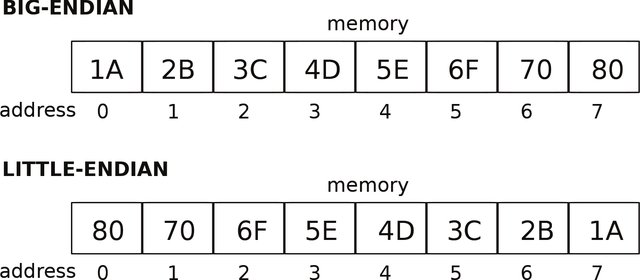
\includegraphics[width=0.7\linewidth]{image/endian}
	\caption{مقایسهٔ اندین کوچک و اندین بزرگ\cite{Grochowski2020}}
	\label{fig:endian}
\end{figure}


\subsection{گره‌ها‌}
گره‌‌های بیت‌کوین را می‌توان با توجه به کاری که انجام می‌دهند به انواع مختلفی دسته‌بندی کرد و طبق \cite{Antonopoulos2016} هر گره می‌تواند مجموعه‌ای از عملکرد‌های مسیریابی، پایگاه‌دادهٔ زنجیره‌ٔ بلوکی، استخراج و کیف پول باشد.
\paragraph{گره کامل}
در این پایان‌نامه منظور از گره کامل گره‌ای است که تمام زنجیرهٔ بلوکی را ذخیره کرده و قادر به مسیریابی و تبادل اطلاعات در شبکهٔ همتا‌به‌همتای بیت‌کوین باشد. گره کامل از بالاترین امنیت ممکن برخوردار بوده و قادر به اعتبارسنجی تمام تراکنش‌ها و بلوک‌ها، بدون افشای اطلاعاتش، است. پیاده‌سازی‌های مختلفی برای گره کامل بیت‌کوین وجود دارد که فرقی در عملکرد آن‌ها وجود ندارد. در این پایان‌نامه، گره کامل نرم‌افزار هستهٔ بیت‌کوین\cite{Bitcoincore.org} را اجرا می‌کند.

\paragraph{گره سبک}

پیاده‌سازی‌های نرم‌افزاری متعددی برای گره سبک یا به عبارت دیگر، کاربر SPV بیت‌کوین وجود دارد. مانند بیت‌کوین‌جی \cite{bitcoinj}، الکترام \LTRfootnote{\lr{Electrum}} 
\cite{Electrum}
و پیکوکوین\LTRfootnote{\lr{PicoCoin}}
\cite{Garzik}. 
اصطلاحا، به نرم‌افزار‌های گره سبک، کیف پول\LTRfootnote{\lr{Wallet}} نیز گفته می‌شود.

بیت‌کوین‌جی یک کتاب‌خانهٔ کاربر سبک (SPV) به زبان
% جاوا \RTLfootnote{\lr{Java}} 
 \gls{Java}
 است. این کیف پول مستقیما با استفاده از پروتکل‌های ارتباطی استاندارد تعریف شده در شبکهٔ همتا‌به‌همتای بیت‌کوین \cite{P2P_dev,P2P_ref} با گره کامل ارتباط برقرار می‌کند. بیت‌کوین‌جی از اکثر استاندارد‌های بیت‌کوین،‌از جمله فیلتر بلوم \cite{Hearn2013}  پشتیبانی می‌کند. در این پایان‌نامه به صورت کلی منظور از گره سبک یا کاربر \lr{SPV}، بیت‌کوین‌جی است. کاربر سبک بیت‌کوین‌جی به صورت همزمان می‌تواند به چند گره کامل متصل باشد و از طریق آن‌ها اطلاعاتش بروزرسانی گردد. کیف‌پول‌ 
بیت‌کوین ولت\LTRfootnote{\lr{Bitcoin Wallet}}، که برای سیستم‌عامل‌های اندروید و بلک‌بری توسعه پیدا کرده است، مثالی از کیف‌پول‌هایی است که از کتاب‌خانهٔ بیت‌کوین‌جی استفاده می‌کنند.

در پیاده‌سازی الکترام،‌ کاربر سبک مستقیما طبق پروتکل ارتباطی بیت‌کوین با گره کامل مبادلهٔ اطلاعات نمی‌کند. گره کاملی که زنجیره بلوکی بیت‌کوین را ذخیره کرده‌است،‌ لازم است برای ارائه خدمات به کاربران سبکی که از الکترام استفاده می‌کنند،‌ سرور 
الکترام‌ایکس\LTRfootnote{\lr{ElectrumX}}
\cite{ElectrumX}
را در کنار نرم‌افزار گره کامل (هسته‌ٔ بیت‌کون) راه‌اندازی نماید. در این پیاده‌سازی، برخلاف بیت‌کوین‌جی، گره سبک هم‌زمان به چند سرور الکترام‌ایکس متصل نمی‌شود. بلکه به صورت تصادفی یک سرور را انتخاب می‌کند و به آن متصل می‌گردد. کاربر سبک خودش می‌تواند تعیین کند که به چه سروری متصل گردد. از این رو کاربر سبک می‌تواند اطلاعاتش را تنها از گره کاملی که به آن اعتماد دارد به روز رسانی نماید.  همچنین در پروتکل ارتباطی گره سبک الکترام با سرور الکترام‌ایکس از فیلتر بلوم استفاده نمی‌شود. این ویژگی‌ها امنیت این پیاده‌سازی را با ابهام مواجه کرده است \cite{Alison2014}. 

پیکوکوین،‌ یک کتاب‌خانه بیت‌کوین به زبان سی\LTRfootnote{\lr{C}} است. این کتاب‌خانه امکان استفاده به عنوان یک کیف‌پول بیت‌کوین و یک گره کامل را فراهم می‌کند. علاوه بر این، امکان ساخت نرم‌افزارهایی که مرتبط با بیت‌کوین هستند را ممکن می‌کند. این کیف پول از استاندارد ارتباطی بیت‌کوین تبعیت کرده و از فیلتر بلوم استفاده می‌کند، همچنین می‌تواند مستقیما به گره‌های کامل بیت‌کوین، بدون نیاز به راه‌اندازی سروری مجزا در سمت گره کامل، متصل شود.

در این پژوهش هرگاه از گره سبک یا کاربر SPV صحبت می‌شود منظور کیف‌پول بیت‌کوین‌جی \cite{bitcoinj} و هر گاه از گره کامل صحبت می‌شود منظور نرم‌افزار
%هستهٔ بیت‌کوین\RTLfootnote{Bitcoin-core} 
\gls{Bitcoin-core}
\cite{Bitcoincore.org}
است.


\subsection{شبکه همتا‌به‌همتای بیت‌کوین}
\label{P2PNetwork}

گره‌های شبکهٔ بیت‌کوین بر اساس یک پروتکل استاندارد با یکدیگر به تبادل پیام می‌پردازند. گره‌های کامل در شبکه بیت‌کوین بعد از آن‌که بلوک‌ها و تراکنش‌های جدید را تصدیق کردند، آن‌ها را به دیگر گره‌ها ارسال می‌کنند. علاوه بر این، گره‌های سبک می‌توانند از پروتکل ارتباطی بیت‌کوین جهت ارتباط با گره‌های کامل استفاده کنند.

تمام  ارتباطات همتا‌به‌همتا در بیت‌کوین در بستر TCP برقرار می‌شوند و تمام پیام‌ها از قالب یکسانی پیروی می‌کنند. رشتهٔ آغازین پیام‌ها و مقدار پیش‌فرض شمارهٔ درگاه با توجه به اینکه پیام در شبکهٔ اصلی، تست یا در حالت تست رگرسیون استفاده می‌شود تفاوت می‌کند. جدول \ref{table:PortandString} این مقادیر را نشان می‌دهد. یک گره می‌تواند از شمارهٔ درگاهی متفاوت در یک شبکه استفاده نماید.



\begin{xltabular}{\textwidth}{|c|c|c|X|}
	\caption{شبکه‌های مختلف بیت‌کوین\label{table:PortandString}}\\
	\hline
	\textbf{شبکه} & \textbf{درگاه پیش‌فرض} & \textbf{رشته‌ٔ آغازین} & \textbf{توضیحات} \\
	\hline \hline 
	اصلی & 8333 & \lr{\texttt{0xf9beb4d9}} & {%
		شبکهٔ اصلی بیت‌کوین.
	}\\
	\lr{Mainnet} & & & {%
		در این شبکه بیت‌کوین دارای ارزش واقعی است.
	} \\
	\hline
	تست & 18333 & \lr{\texttt{0x0b110907}} & {%
		شبکهٔ آزمایشی بیت‌کوین
	}\\
	\lr{Testnet} & & & {%
		برای توسعه دهندگان بهتر و کم هزینه‌ تر است که از شبکهٔ آزمایشی بیت‌کوین استفاده کنند. چرا که بیت‌کوین‌ در آن دارای ارزش واقعی نیست.
	} \\
	\hline
	تست رگرسیون & 18444 & \lr{\texttt{0xfabfb5da}} & {%
		حالت تست رگرسیون
	}\\
	\lr{Regtest} & & & {%
		گاهی در توسعه یک کاربرد نیازی نیست که با گره‌های تصادفی در ارتباط باشیم یا بلوک‌های تصادفی تولید شده را بررسی کنیم. در این شرایط از حالت تست رگرسیون بیت‌کوین استفاده می‌کنیم. در این حالت می‌توان محیط را کنترل کرد و تعیین کرد که چه زمانی یک بلوک جدید ساخته شود.
	} \\
	\hline
	
	
\end{xltabular}


علاوه بر این تمام پیام‌های شبکه‌ٔ همتا‌به‌همتای بیت‌کوین شامل سرایندی یکسان هستند که قالب این سرایند مطابق جدول \ref{table:p2pheader} است.

\begin{xltabular}{\textwidth}{|c|X|}
	\caption{قالب سرایند تمام‌ پیام‌ها در شبکهٔ همتا‌به‌همتای بیت‌کوین \label{table:p2pheader}}\\ \hline
	\textbf{نام} & {\textbf{توضیحات} } \\
	\hline \hline
	\lr{start string}&{%
		بایت‌هایی که در جدول \ref{table:PortandString} توضیح داده شد که نشان دهندهٔ شبکه‌ای است که این پیام در آن تولید شده است.
	}\\
	\hline
	
	\lr{command name} & {%
		رشته‌ای در استاندارد 
%		اَسکی
		\gls{ASCII}\LTRfootnote{ASCII}
		است که مشخص می‌کند چه نوع پیامی در 		
		\gls{Payload}\LTRfootnote{Payload}
		قرار گرفته است. اندازهٔ این قسمت ۱۲ کاراکتر است و بایت‌های بعد از نام پیام برابر صفر (\texttt{0x00}) خواهند بود. به عنوان مثال برای پیام \texttt{Version} خواهیم داشت:
		\lr{\texttt{version\textbackslash0\textbackslash0\textbackslash0\textbackslash0\textbackslash0}}.
	}\\
	\hline
	
	\lr{payload size} & {%
		اندازه بایت‌های پیام داخل پایه‌بار را مشخص می‌کند. حداکثر تعداد بایت‌ مجاز در پایه‌بار ۳۲ مگابایت‌ (\lr{‍‍``MAX\_SIZE''}) است. پیام‌های بزرگ‌تر از این مقدار دورانداخته می‌شوند. پیام‌هایی مانند \texttt{VerAck}   بدون پایه‌بار هستند.
	}\\
	\hline
	
	\lr{checksum} & {%
		چهار بایت اول حاصل 
		\lr{SHA256(SHA256(payload))}
		است. اگر پایه‌بار خالی باشد، مانند پیام‌های \texttt{VerAck} و \texttt{GetAddr}، مقدار این بخش برابر 
		\lr{\texttt{0x5df6e0e2}}
		بوده که معادل 
		\lr{SHA256(SHA256(
			\rl{رشتهٔ خالی}
			))}
		است.
	}\\
	\hline
	
\end{xltabular}  

\subsubsection{یافتن همتا}

اولین گامی که هر گره در شبکهٔ همتا‌به‌همتای بیت‌کوین انجام می‌دهد، یافتن گره‌های (همتا‌های) دیگر و اتصال به آن‌ها است. از آن‌جایی که یک گره در زمان راه اندازی، آدرس آی‌پی گره‌های کامل فعال را ندارد، از یک یا چند سرور 
\LTRfootnote{\lr{Domain Name System}}\lr{DNS} 
که آدرس‌ آن‌ها در کد بیت‌کوین‌جی از پیش قرارگرفته است پرسمان انجام می‌دهد. پاسخ دریافت شده شامل آدرس یک یا چند گره کامل است که ارتباطات ورودی را قبول می‌کنند. علاوه بر این تعدادی آدرس گره کامل در هر ورژن از کدهای بیت‌کوین‌جی قرار دارد که در زمانی که آن ورژن مشخص منتشر می‌شده فعال بوده‌اند. 
\subsubsection{اتصال به همتا}
بعد از آن‌که کاربر جدید آدرس آی‌پی یک یا چند گره کامل را بدست آورد، برای آن گره‌(ها) پیام \texttt{version} را ارسال می‌کند. این پیام برای ایجاد ارتباط ارسال می‌شود و شامل اطلاعاتی از گره ارسال کننده است. این اطلاعات در جدول \ref{table:VersionMessage} توضیح داده شده است. گره دریافت کننده نیز یک پیام \texttt{version} را که شامل اطلاعات خودش است، ارسال می‌کند. هر دو گره به محض دریافت پیام \texttt{version} پیام \texttt{verack} را برای گره مقابل ارسال می‌نماید. پیام \texttt{verack} بدون
%پایه‌بار\RTLfootnote{Payload}
\gls{Payload}
است و به گره دریافت کننده اطلاع می‌دهد که آماده دریافت پیام‌‌های بعدی است.


\begin{xltabular}{\textwidth}{|c|X|}
	\caption{
		قسمت‌های پیام \texttt{version} در شبکه همتا‌به‌همتای بیت‌کوین
		\label{table:VersionMessage}}\\
	\hline
	\textbf{نام} & {\centering
		\textbf{توضیحات}		
	} \\
	\hline
	\hline
	\lr{version} & {
		بالاترین نسخهٔ پروتکلی که توسط گره ارسال کننده شناخته می‌شود.	در زمان نگارش این پایان‌نامه، بالاترین نسخه پروتکل بیت‌کوین 70015 است که در سال ۲۰۱۷ منتشر شده است.
	} \\
	\hline
	\lr{services} & {
		خدماتی که گره ارسال‌کننده پشتیبانی می‌کند را مشخص می‌کند. برای گره‌های سبکی مثل بیت‌کوین‌جی، مقدار آن برابر \texttt{0x00} است.
	} \\
	\hline
	\lr{timestamp} & {
%		ساعت یونیکس\RTLfootnote{\lr{Unix time}} 
		\gls{Unix time}\LTRfootnote{\lr{Unix time}}
		با توجه به ساعت گره ارسال کننده در زمان ارسال پیام.
	} \\
	\hline
	\lr{addr\_recv services} & {
		سرویس‌هایی که از دید گره ارسال‌کننده، توسط گره گیرنده پشتیبانی می‌شود. فرمت نمایش آن مانند قسمت services است. اگر گره ارسال‌کننده، بیت‌کوین‌جی باشد، همیشه به صورت پیش‌فرض مقدار این قسمت را برابر \texttt{0x00} قرار می‌دهد.
	} \\
	\hline
	\lr{addr\_recv port} & {
		شماره پورت گره گیرنده از دید گره ارسال‌کننده.
	}\\
	\hline
	\lr{addr\_trans services} & {
		خدماتی که گره ارسال‌کننده پشتیبانی می‌کند را مشخص می‌کند. یکسان با قسمت services باید باشد.
	}\\
	
	\hline
	\lr{addr\_trans IP address} & {
		آدرس آی‌پی گره ارسال کننده.
	}\\
	
	\hline
	\lr{addr\_trans port} & {
		شماره پورت گره ارسال کننده.
	}\\
	
	\hline
	\lr{nonce} & {
		تک‌شمار، یک عدد تصادفی است که اگر یک گره،‌ یک پیام با تک‌شماری مشابه با تک‌شمار ارسالی دریافت کرد، ارتباط را قطع نماید. (قسمت تک‌شمار در نسخهٔ \lr{$0.1.6$} بیت‌کوین اضافه شده و هدفش آن است که گره متوجه شود که به خودش متصل نشده باشد)
		\LTRfootnote{  \lr{\url{https://github.com/bitcoin/bitcoin/commit/cc0b4c3b62367a2aebe5fc1f4d0ed4b97e9c2ac9}}}.
	}\\
	\hline
	\lr{user\_agent bytes} & {
		تعداد بایت‌هایی که پیام قسمت \lr{user\_agent} (قسمت بعدی) استفاده کرده است.
	}\\
	
	\hline
	\lr{user\_agent} & {
		نوع برنامه کاربر را معین می‌کند. مثلا:
	}\\
	
	&  {%
		۱. بیت‌کوین‌جی: 
		\lr{/bitcoinj:1.0/MultiBit:1.0(Windows)/}} \\
	&  {%
		۲. هستهٔ بیت‌کوین (گره کامل): 
		\lr{/Satoshi:0.20.0/(70015)/}} \\
	
	\hline
	\lr{start\_height} & {
		ارتفاع بهترین زنجیره‌ بلوکی گره ارسال کننده در این قسمت قرار گرفته می‌شود. در صورتی که کاربر SPV باشد، ارتفاع بهترین زنجیره سرایند بلوک‌‌ها قرار داده می‌شود.
	}\\
	
	\hline
	\lr{relay} & {
		قرار دادن این بخش در پیام اختیاری است. این بخش در \cite{Hearn2013} به همراه پیشنهاد استفاده از فیلتر بلوم در بیت‌کوین معرفی شده است. مقدار آن صحیح (\texttt{0x01}) یا غلط (\texttt{0x00}) است. در صورتی که صحیح باشد، یا از آن استفاده نشود، تغییری در پروتکل ایجاد نمی‌شود. ولی در صورتی که غلط باشد، قبل از آن‌که کاربر ارسال کننده، پیام‌های \texttt{filterload} و \texttt{filterclear} را ارسال کرده باشد، هیچ پیام \texttt{inv} یا \texttt{tx} به آن ارسال نمی‌شود. این کار باعث می‌شود که در فاصلهٔ زمانی انجام 
%		دستداد \RTLfootnote{Handshake}
		\gls{Handshake}\LTRfootnote{Handshake}
		(ارسال پیام \texttt{version}) و فرستادن فیلتر بلوم، کاربر سبک تحت سیل پیام‌های گره‌کامل قرار نگیرد. 
	}\\
	
	
	\hline
\end{xltabular}

زمانی که اتصال با یک گره کامل برقرار شد، پیام \texttt{getaddr} برای گره کامل فرستاده می‌شود تا آدرس آی‌پی گره‌های کامل فعالی که گره دریافت‌کننده به آن‌ها متصل است در قالب پیام \texttt{addr} برای گره فرستنده ارسال شود. گره فرستنده همتا‌های فعال خودش را نیز در قالب پیام \texttt{addr} برای گره کامل گیرنده ارسال می‌کند.

\subsubsection{هم‌گام سازی گره سبک}
از این قسمت به بعد تنها به بررسی فعالیت‌های گره سبک در شبکه می‌پردازیم و هم‌گام‌سازی دیگر گره‌های شبکه مورد بررسی قرار نمی‌گیرند. کاربر سبک بعد از اتصال اولیه به یک گره کامل، نیاز دارد که سرایند بلوک‌های زنجیرهٔ بلوکی را دریافت نماید به این کار 
%هم‌گام‌سازی \RTLfootnote{Synchronization}
 \gls{Synchronization}
 گفته می‌شود. همان‌طور که گفته شد کاربر سبک به جای ذخیره‌سازی و تصدیق تمام زنجیرهٔ بلوکی،‌ تنها سرایند آن را ذخیره می‌کند. حجم سرایند یک بلوک $80$ بایت است. در گره‌های کامل، که می‌خواهند تمام زنجیره بلوکی را دریافت نمایند، این فرایند به دو صورت
%«ابتدا-بلوک\RTLfootnote{Blocks-First}»
«\gls{Blocks-First}»
یا
«\gls{Headers-First}»
قابل انجام است که در این‌جا به توضیح آن‌ها پرداخته نمی‌شود. گره سبک در گام اول هم‌گام‌سازی لازم است که 
%بهترین سراید زنجیرهٔ بلوکی \RTLfootnote{\lr{Best header chain}} 
\gls{Best header chain}
را دانلود کند. سرایند زنجیرهٔ بلوکی، زنجیره‌ای از سرایند بلوک‌ها است که هر کدام از سرایند‌ها به سرایند بلوک قبل خود اشاره می‌کند. بهترین سرایند زنجیرهٔ بلوکی، زنجیره‌ای است که دشوارترین بازآفرینی را داشته باشد. 

گره سبک برای دریافت سرایند زنجیرهٔ بلوکی، پیام \texttt{getheaders} را برای گره کاملی (گره هم‌گام‌ساز) که می‌خواهد با آن همگام شود ارسال می‌کند. جدول \ref{table:GetHeadersMessage} بخش‌های مختلف این پیام را توضیح می‌دهد و شکل \ref{fig:getheaders} مثالی از یک پیام \texttt{getheaders} است که گره سبک برای اولین‌بار برای گره هم‌گام‌ساز ارسال می‌کند.



\begin{xltabular}{\textwidth}{|c|X|}
	\caption{
		قسمت‌های پیام \texttt{getheaders} در شبکه همتا‌به‌همتای بیت‌کوین
		\label{table:GetHeadersMessage}}\\
	\hline
	\textbf{نام} & {\textbf{توضیحات}} \\
	\hline \hline
	\lr{version} & {%
		شماره‌ٔ نسخه‌ٔ پروتکل. شبیه آنچه در پیام \texttt{version} ارسال شد.
	} \\
	
	\hline
	
	\lr{hash count} & {%
		تعداد چکیده‌هایی که در بخش بعدی پیام قرار می‌گیرند، در این قسمت تعیین می‌شوند. محدودیتی در تعداد چکیده‌های ارسالی نیست. اما اندازه کل پیام باید کمتر از \lr{‍‍``MAX\_SIZE''} (۳۲ مگابایت) باشد.
	} \\
	\hline
	
	
	\lr{block header hashes} & {%
		چکیدهٔ یک یا چند سرایند بلوکی که گره ارسال کننده آن‌ها را در حافظهٔ خود دارد. ترتیب چکیده‌ها از بالاترین ارتفاع بلوک (جدید‌ترین) به پایین‌ترین ارتفاع است. به این ترتیب به گره دریافت‌کننده‌ٔ پیام این امکان داده می‌شود که جدیدترین چکیدهٔ سرایندی که با هم مشترک هستند را پیدا کند. اگر گره سبکش تازه راه‌اندازی شده‌ باشد در این قسمت، چکیدهٔ بلوک جنسیس (\lr{6fe2…0000}) را که در نرم‌افزارش از ابتدا وجود داشته است، قرار می‌دهد.
	} \\
	\hline
	
	\lr{stop hash} & {%
		این قسمت چکیدهٔ آخرین بلوکی است که گره ارسال‌کننده می‌خواهد دریافت کند. با صفر قراردادن آن، طولانی‌ترین پاسخ ممکن از گره کامل تقاضا می‌شود. حداکثر تعداد سرایندی که گره کامل دریافت کنندهٔ این پیام پاسخ می‌دهد، $2000$ سرایند است. برای دریافت بیشتر از این مقدار، این پیام در چند نوبت ارسال می‌شود
	}\\
	\hline
	
\end{xltabular}

\begin{figure}[h]
	\centering
	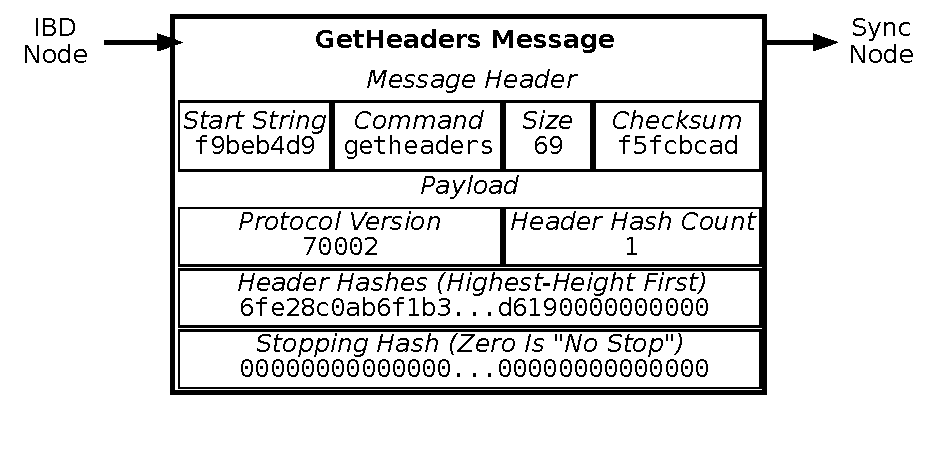
\includegraphics[width=0.7\linewidth]{image/getheaders}
	\caption{مثالی از پیام \texttt{getheaders} در همگام‌سازی اولیهٔ یک گره جدید}
	\label{fig:getheaders}
\end{figure}


گره هم‌گام‌ساز در پاسخ به پیام \texttt{getheaders} در شکل \ref{fig:getheaders} دنبال بلوکی با چکیده مشخص شده می‌گردد و می‌یابد که این بلوک برابر بلوک شمارهٔ صفر (بلوک جنسیس) است. به این ترتیب $۲۰۰۰$ سرایند بلوک را که از بلوک شمارهٔ یک آغاز می‌شوند در قالب پیام \texttt{headers} برای گره درخواست دهنده ارسال می‌کند. قالب این پیام در جدول \ref{table:HeadersMessage} مشخص شده‌ است. شکل \ref{fig:headers} مثالی از پیام بازگردانده شده توسط گره هم‌گام‌ساز است.

\begin{table}[!h]
	\centering
	\caption{
		قسمت‌های پیام \texttt{headers} در شبکه همتا‌به‌همتای بیت‌کوین
		\label{table:HeadersMessage}}
	\begin{tabular}{|c|r|}
		\hline
		\textbf{نام} & {\textbf{توضیحات}} \\
		\hline \hline
		
		\lr{count} & {%
			تعداد سرایند‌های بلوک قرار گرفته در بخش بعدی این پیام. (حداکثر $2000$)
		} \\
		\hline
		
		\lr{headers} & {%
			سرایند‌ بلوک‌ها در این قسمت قرار می‌گیرند.
		} \\
		\hline
	\end{tabular}
\end{table}

\begin{figure}[!h]
	\centering
	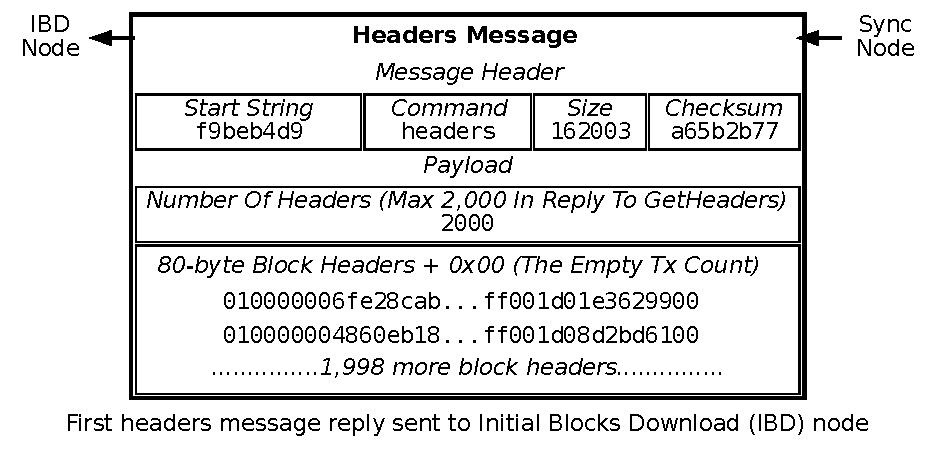
\includegraphics[width=0.7\linewidth]{image/headers}
	\caption{مثالی از پیام \texttt{headers} در همگام‌سازی اولیهٔ یک گره جدید}
	\label{fig:headers}
\end{figure}

وقتی گره سبک پاسخ شکل \ref{fig:headers} را دریافت کرد، فورا صحت آن را بررسی کرده و مجددا پیام  \texttt{getheaders} جدیدی برای گره همگام‌ساز برای گرفته باقیمانده سرایند‌ها ارسال می‌کند. این فرایند تا گرفتن کامل سرایند‌ها ادامه پیدا می‌کند. در زمان نوشتن این پایان‌نامه، حجم تمام سرایند‌های زنجیرهٔ بلوکی ۵۰ مگابایت است. پس از اتمام دانلود سرایند‌های زنجیرهٔ  بلوکی، گره سبک آخرین پیام \texttt{getheaders} را برای چند همتای دیگر ارسال کرده و پاسخ آن‌ها را با پاسخ گره هم‌گام‌ساز ابتدایی مقایسه می‌کند. به این ترتیب مطمئن می‌شود که بهترین سرایند زنجیرهٔ بلوکی را دریافت کرده است. 

\subsubsection{انتشار}

زمانی که گره کامل یک بلوک جدید را دریافت می‌کند، پیام \texttt{inv} را برای همهٔ همتا‌هایش (چه گره کامل چه گره سبک) ارسال می‌کند. پیام ارسال شده دارای یک 
%مدخل فهرست \RTLfootnote{Inventory} 
\gls{Inventory}
مربوط به بلوک جدید است. یک مدخل فهرست، شامل یک علامت نوع داده و یک  چکیده داده به عنوان مشخص‌کنندهٔ آن است. داده می‌تواند انواع مختلفی داشته باشد، به عنوان نمونه، علامت تراکنش
\lr{``MSG\_TX''}
و علامت بلوک
\lr{``MSG\_BLOCK''}
است.
 به صورت کلی مدخل فهرست به وجود تراکنش‌ها یا بلوک‌هایی برای دانلود اشاره می‌کند. جدول \ref{table:InvMessage} قسمت‌های مختلف پیام \texttt{inv} را شرح می‌دهد. 

\begin{xltabular}{\textwidth}{|c|X|}
	\caption{
		قسمت‌های پیام \texttt{inv} در شبکه همتا‌به‌همتای بیت‌کوین
		\label{table:InvMessage}}\\
	\hline
	\textbf{نام} & {\textbf{توضیحات}} \\
	\hline \hline
	
	\lr{compactSize uint} & {%
	تعداد مدخل‌های فهرست. 
}\\
\hline

	\lr{inventory} & {%
	یک یا چند مدخل فهرست. حداکثر تعداد آن می‌تواند $50000$ باشد. به عنوان مثال محتوای این قسمت از پیام برای اطلاع‌رسانی بلوک ارتفاع 
	$645747$\LTRfootnote{\url{https://blockchair.com/bitcoin/block/645747}}
	به گره‌های همتا به این صورت است: 
}\\

&{%
علامت نوع داده:
\lr{MSG\_BLOCK}
}\\

&{%
مشخص‌کنندهٔ داده (چکیده):
\lr{\texttt{0x333ab9f10d...0000000000}}
}\\

\hline

\end{xltabular}

گره سبک بعد از دریافت این پیام، یک پیام \texttt{getdata} برای گره کامل می‌فرستد. در این پیام درخواست می‌کند که با توجه به فیلتر بلومی که پیش‌تر در اختیار گره کامل گذاشته بوده، تراکنش‌هایی از بلوک جدید را، که در آن فیلتر صدق می‌کنند برای اون بفرستد. ساختار پیام \texttt{getdata} شبیه \texttt{inv} است. با این تفاوت که علامت نوع داده،‌ اطلاعاتی است که گره ارسال کننده این پیام از گره دریافت‌کننده درخواست می‌کند. 
در این کاربرد، گره سبک علامت \lr{‍‍‍``MSG\_FILTERED\_BLOCK''}  را در کنار چکیده‌ٔ بلوک مورد نظر در پیام قرار می‌دهد و برای گره کامل ارسال می‌کند. به این ترتیب گره کامل تراکنش‌هایی که حداقل یک آدرس آن‌ها در فیلتر بلوم صدق می‌کنند را در کنار اثبات مرکل آن‌ها برای گره سبک ارسال می‌کند.
پاسخ در قالب یک پیام \texttt{merkleblock} که شامل اثبات مرکل وجود تراکنش‌های مرتبط در بلوک است و تعداد صفر یا چند پیام \texttt{tx} را که خود تراکنش‌ها هستند خواهد بود. 

به خاطر ماهیت فیلتر بلوم، پاسخ گره کامل  شامل تراکنش‌هایی می‌شود که مورد توجه گره سبک نیستند. این اتفاق منجر به گمراه شدن گره کامل در شناخت تراکنش‌های مرتبط با گره سبک می‌شود. هدف از این کار حفظ گم‌نامی کاربر سبک و فاش نشدن آدرس وی نزد گره کامل است. در قسمت \ref{BloomFilter} علاوه بر توضیح فیلتر بلوم، نحوه استفاده از آن در شبکهٔ همتابه‌همتا، مثل ارسال آن برای گره کامل  از طریق ارسال پیام \texttt{filterload} و نحوهٔ تولید پیام \texttt{merkleblock}  توسط گره کامل و ساختار آن توضیح داده می‌شود. همچنین، در این قسمت در مورد آسیب‌پذیری‌های فیلتر بلوم و ناتوانی آن در حفظ حریم خصوصی کاربران بحث خواهد شد.


\section{فیلتر بلوم}
\label{BloomFilter}
فیلتر بلوم را نخستین بار برتون بلوم در \cite{Bloom1970} معرفی کرد. هدف این فیلتر امتحان سریع وجود یک عضو در یک مجموعه است. فیلتر بلوم کاربرد گسترده‌ای در پایگاه‌های داده، شبکه و حتی موتور‌های جست‌وجو دارد. فیلتر بلوم آرایه‌ای از $n$ بیت $b[i]$ است که $i$ از $0$ تا$n-1$ است. به صورت پیش‌فرض تمام بیت‌ها مقدار صفر دارند. اگر بخواهیم عضو $x$ را (مثلا یک رشته) درون مجموعه آن قرار دهیم، آن عضو را در ورودی $k$ تابع چکیده‌ساز مستقل
$H_1(.), H_2(.), ..., H_k(.)$
قرار می‌دهیم. خروجی هر تابع چکیده ساز یک عدد صحیح بین $0$ تا $n-1$ است. از این رو هر تابع چکیده ساز، یک عنصر ورودی را به یکی از	 $n$ بیت فیلتر بلوم نگاشت می‌کند. برای قرار دادن آن رشته در مجموعه مربوط به فیلتر بلوم، بیت متناظر عدد حاصل را برابر با یک قرار می‌دهیم: 

$\forall j\in \{1..k\}, b[H_j(x)] \leftarrow 1$.

به همین ترتیب اگر بخواهیم بررسی کنیم که یک رشته در مجموعه قرار دارد، چکیده آن رشته را توسط همان $k$ تابع چکیده‌ساز حساب نموده و بررسی می‌کنیم که آیا مقدار ذخیره شده در تمام $k$ جایگاه بدست آمده برابر یک است یا خیر. اگر برابر با یک باشد، آن رشته را عضو احتمالی آن مجموعه در نظر می‌گیریم. به آن عضو احتمالی گفته می‌شود چرا که ممکن است عناصری عضو مجموعه نباشند و به جایگاه‌هایی که مقدار  بیت آن‌ها برابر با یک است نگاشت شوند. به این ترتیب امکان بروز خطای نوع دو وجود دارد. مجموعهٔ تمامی عناصر با $\mathcal{U}$، اعضایی که درون فیلتر بلوم قرار گرفته‌اند با $\mathcal{S}$ و مجموعهٔ عناصری که در نتیجه خطای نوع دو عضو فیلتر بلوم در نظر گرفته می‌شوند با $\mathcal{V}$ نمایش داده می‌شوند. به صورت کلی می‌توان گفت هرگاه لیست یا مجموعه‌ای مورد استفاده قرار گرفت، هزینه فضای ذخیره‌سازی و دسترسی به اعضای مجموعه قابل توجه بود و خطای نوع دو خسارت و هزینه چندانی به سامانه تحمیل نکند، استفاده از فیلتر بلوم مفید خواهد بود. فیلتر بلوم امکان انجام مصالحه بین فضای استفاده شده، زمان پاسخ‌گویی و احتمال خطای قابل قبول را فراهم می‌کند\cite{Bloom1970}. با توجه به ساختار فیلتر بلوم روشن است که امکان بروز خطای نوع یک، یا به عبارت دیگر امکان آنکه عضو مجموعه را غیر عضو تشخیص دهد، وجود ندارد.

\begin{figure}
	\centering
	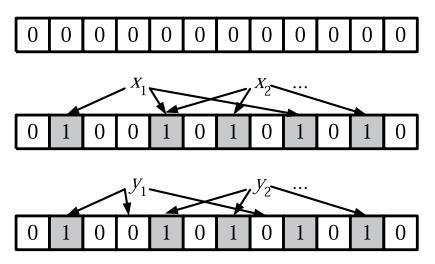
\includegraphics[width=0.55\linewidth]{image/BloomFilter}
	\caption[نمونه‌ای از عمکلرد فیلتر بلوم]{
		فیلتر مجموعه بدون عضو متشکل از یک آرایه‌ از بیت‌ها با مقدار صفر است. k دفعه چکیده هر عضو مجموعه $x_i$ محاسبه می‌شود که حاصل هر چکیده موقعیت یک بیت است. که مقدار این بیت‌ها ۱ می‌شود. حال برای آنکه بررسی کنیم که $y_i$ درون این مجموعه است به تعداد k بار از آن چکیده می‌گیریم و بیت‌های مرتبط را بررسی می‌کنیم. عنصر $y_1$ نمی‌تواند عضو مجموعه باشد چرا که یکی از بیت‌هایی که به آن اشاره می‌کند صفر است. عنصر $y_2$ یا عضو مجموعه است یا اینکه به خاطر خطای نوع دو فیلتر، عضو مجموعه تشخیص داده شده است.\cite{Broder2004}
	}
	\label{fig:bloomfilter}
\end{figure}

در فیلتر بلوم برای تنظیم نرخ قابل قبول خطای نوع دوم ($P_t$)، با توجه به حداکثر تعداد عناصری که در فیلتر قرار خواهند گرفت($M$)، اندازه فیلتر($n$) و تعداد توابع‌ چکیده‌ساز($k$) تعیین می‌شوند.
جدول \ref{table:BloomFilter} نشانه‌گذاری‌های مربوط به فیلتر بلوم را نشان می‌دهد.

\begin{table}[h]
	\centering
	\caption{قرارداد نشانه‌گذاری برای فیلتر بلوم}
	\label{table:BloomFilter}
	\begin{tabular}{|c|c|}
		\hline
		نشانه‌گذاری & معنا \\
		\hline
		\hline
		$\mathcal{S}$ & مجموعه عناصری که عضو فیلتر شده‌اند \\
		\hline
		$M$ & حداکثر تعداد عناصر فیلتر\\
		\hline
		$m = |\mathcal{S}|$ & تعداد عناصر قرار داده شده در فیلتر\\
		\hline
		$n$ & اندازه (تعداد بیت‌های) فیلتر \\
		\hline
		$k$ & تعداد توابع چکیده‌ساز\\
		\hline
		$\mathcal{U}$ & مجموعهٔ تمام عناصر، $|\mathcal{U}| = N_u$ \\
		\hline
		$\mathcal{V}$ & مجموعهٔ پنهان‌سازی (عناصر خطای نوع دو)، $|\mathcal{V}| = N_v$\\
		\hline
		$P_t$ & نرخ (احتمال) خطای نوع دوی هدف (ایده‌آل)\\
		\hline
		$P_f$ & نرخ (احتمال) خطای نوع دوی واقعی \\
		\hline
		$B(M, P_t)$ & فیلتر بلوم با حداکثر ظرفیت $M$ و نرخ خطای نوع دو هدف $P_t$ \\
		\hline
	\end{tabular}
\end{table}

برای فیلتر بلوم
$B(M, P_t)$
اندازه فیلتر به صورت زیر محاسبه می‌شود\cite{Gervais2014}:

\begin{equation}
n=-\frac{M\ln(P_t)}{\left(\ln(2)\right)^2} \label{eq:n_of_bloom_filter}
\end{equation}
و تعداد توابع چکیده‌ساز به صورت زیر محاسبه می‌گردد\cite{Gervais2014}:
\begin{equation}
k=\ln(2)\frac{n}{M} \label{eq:k_of_bloom_filter}
\end{equation}
احتمال خطای نوع دو فیلتر بلوم
$B(M, P_t)$
، در صورتی که $m$ عنصر در آن قرار دهیم که
$m<M$
، کمتر از مقدار هدف آن ($P_t$) می‌شود. اگر بیشتر از ظرفیت یک فیلتر در آن عنصر قرار داده شود،‌نرخ خطای نوع دو آن از از احتمال هدف بیشتر می‌گردد.

احتمال خطای نوع دو در یک فیلتر با توجه به عناصری که در آن قرار داده شده است، ($m$) با دقت‌های متفاوتی محاسبه شده است. مقاله \cite{Bloom1970}، که فیلتر بلوم را معرفی کرده است، احتمال خطای نوع دو را برای فیلتر بلوم محاسبه کرده است. این مقاله با فرض این‌که بعد از قرار دادن $m$ عضو در فیلتر بلوم نسبت بیت‌هایی که مقدار آن‌ها صفر مانده است به کل بیت‌ها برابر
$(1-k/n)^m$
باشد، احتمال خطای نوع دو را به صورت زیر محاسبه کرده است:

\begin{equation}
P_f(m) = \left(1-\left(1-\frac{k}{n}\right)^{m}\right)^k \label{eq:Pf_of_bloom_filter_Bloom}
\end{equation}

در مقاله \cite{Mullin1983} محاسبه دقیق‌تری از احتمال خطای نوع دو به دست آمده است. در این مقاله، احتمال آن که یک بیت دلخواه بعد از مقدار دهی k بیت مقدارش عوض نشود،
$(1-1/n)^k$
محاسبه شده است. پس به این ترتیب بعد از قرار دادن $m$ عضو در فیلتر، احتمال آن‌که مقدار یک بیت تغییر نکند، برابر 
$(1-1/n)^{km}$
خواهد بود. در نتیجه احتمال آن‌که مقدار یک بیت تغییر کند به صورت 
$p_{set} = 1-(1-1/n)^{km}$
محاسبه می‌شود. پس احتمال خطای نوع دو برابر است با احتمال آن‌که تمام بیت‌های انتخابی حاصل از $k$تا چکیدهٔ عنصری که عضو فیلتر بلوم مورد نظر نیست،‌ از قبل مقدار یک گرفته باشند. به این ترتیب احتمال خطای نوع دو طبق اثبات \cite{Mullin1983}، به صورت زیر محاسبه می‌شود.

\begin{equation}
P_f(m) = \left(1-\left(1-\frac{1}{n}\right)^{km}\right)^k \approx \left(1-e^{-\frac{mk}{n}}\right)^k
\label{eq:Pf_of_bloom_filter_Mullin}
\end{equation}

برای $n\gg k$، مقادیر معادله‌های  \eqref{eq:Pf_of_bloom_filter_Mullin} و \eqref{eq:Pf_of_bloom_filter_Bloom} به هم نزدیک خواهند بود. مقاله \cite{Christensen2010} به فرمولی با دقت بیشتر از دو مقاله قبلی برای محاسبه احتمال خطای نوع دوی فیلتر بلوم دست پیدا کرده است که به شرح زیر است:

\begin{equation}
P_f(m) = \frac{n!}{n^{k(m+1)}} \sum_{i=1}^{n} \sum_{j=1}^{i} (-1)^{i-j} \frac{j^{km}i^k}{(n-i)!j!(i-j)!}
\label{eq:Pf_of_bloom_filter_Christensen}
\end{equation}


اثبات فرمول \eqref{eq:Pf_of_bloom_filter_Christensen} خارج از بحث این پایان‌نامه است. اگر تعداد پیام‌های قرارداده شده در فیلتر بلوم برابر با $M$ باشد، در آن صورت 
$P_f(M)=P_t$.


کاربرد‌های متعددی برای فیلتر بلوم وجود دارد و در ادامه یکی از آن‌ها را مرور خواهیم کرد. در وبسایت‌هایی که خدمات کوتاه‌کردن لینک را ارائه می‌کنند (مانند \cite{Bitly.comTeam2020})، معمولا لیست سیاهی از آدرس‌های غیر امن نگهداری می‌شود و به کاربر استفاده کننده از لینک‌های کوتاه‌شده اطمینان می‌دهد که آدرسی که به آن هدایت خواهد شد یک آدرس امن است (در لیست سیاه آدرس‌های ناامن قرار ندارد). جست‌وجو کردن لیست سیاه آدرس‌های ناامن برای هر درخواست امری زمان‌بر است. از این رو، مجموعهٔ تمام آدرس‌های ناامن در یک فیلتر بلوم نگهداری می‌شود. اگر پاسخ فیلتر بلوم برای یک آدرس درخواست داده شده منفی باشد (عضو مجموعه نباشد) می‌توانیم صددرصد مطمئن باشیم که آدرس در‌خواست داده شده یک آدرس امن است و اگر پاسخ مثبت باشد،‌ جهت جبران خطای نوع دو، پایگاه‌ داده لیست سیاه آدرس‌های ناامن را جست‌وجو می‌کند\cite{Azar2016}.

کاربرد فیلتر بلوم مورد نظر در این پایان‌نامه، استفاده از آن در گره‌های سبک برای حفظ گم‌نامی این گره‌ها است \cite{Hearn2013}. در بخش‌  \ref{BloomFilterInP2P} به نحوهٔ استفاده از این فیلتر در ارتباط بین گره‌های سبک و گره‌های کامل پرداخته می‌شود و در بخش \ref{Vulnerabilities} به ضعف‌ها و آسیب‌پذیری‌های استفاده از این فیلتر در شبکه بیت‌کوین خواهیم پرداخت. 


\subsection{فیلتر بلوم در شبکهٔ همتا‌به‌همتای بیت‌کوین}
\label{BloomFilterInP2P}

امکان استفاده از فیلتر بلوم در ارتباط بین گره سبک و گره کامل به دنبال معرفی آن در طرح پیشنهادی بهبود بیت‌کوین شمارهٔ ۳۷ (\lr{BIP37}) \cite{Hearn2013} در سال ۲۰۱۳ فراهم شد.  گره‌‌های سبک برای حفظ گم‌نامی خود، به جای آن‌که آدرس‌های مربوط به خودشان را صورت فاش در اختیار یک گره کامل قراردهند، آدرس‌های خود و دیگر اطلاعات مورد نیازشان را در یک فیلتر بلوم با نرخ خطای نوع دوی معین قرار می‌دهند. گره کامل با تطابق داده‌های داخل تراکنش‌ها با فیلتر بلوم بررسی می‌کند آن داده درون فیلتر بلوم صدق می‌کند یا خیر. اگر یک داده درون فیلتر بلوم صدق کرد، گره کامل آن داده را برای گره سبک ارسال می‌کند. به صورت کلی اطلاعاتی که می‌توانند درون فیلتر بلوم قرار بگیرند و توسط گره کامل با فیلتر بلوم تطابق داده می‌شوند می‌شوند به صورت زیر است:
\begin{enumerate}
\item{%
چکیدهٔ تراکنش‌ (\lr{TXID})}
\item{%
برای هر خروجی تراکنش، داده‌های
%نبشتهٔ\RTLfootnote{Script} 
\gls{Script}
خروجی بررسی می‌شوند. این داده‌ها نظیر \lr{pubKeyHash} یا \lr{pubKey} هستند. زمانی که یکی از این داده‌ها با فیلتر بلوم تطابق پیدا کنند، گره کامل، در صورت درخواست کاربر، مintی‌تواند دادهٔ \lr{COutPoint} را به فیلتر اضافه نماید. به این‌ترتیب فیلتر را به‌روزرسانی کند.
}
\item{%
برای هر ورودی، \lr{COutPoint} بررسی می‌شود.
}
\item{%
برای هر ورودی، داده‌های نبشتهٔ ورودی بررسی می‌شوند. این داده‌ها نظیر 
\lr{pubKey}
یا
\lr{sig} 
هستند.
}
\end{enumerate} 

اگر گره‌کامل بتواند در یک تراکنش مطابقتی بین هر کدام از موارد بالا و فیلتر بلوم پیدا کند آن تراکنش را برای گره سبک ارسال می‌کند. در غیر این صورت چیزی برای گره سبک ارسال نمی‌شود. در ادامه، به بررسی پروتکل ارتباطی گره‌های سبک با گره‌های کامل و گرفتن اثبات مرکل  برای تراکنش‌های مورد نظر کاربر سبک با بهره‌گیری از فیتلر بلوم پرداخته خواهد شد. 

در قسمت \ref{P2PNetwork}، نحوهٔ اتصال یک گره سبک به گره‌های فعال شبکه‌ٔ همتا‌به‌همتای بیت‌کوین توضیح داده شد. در این قسمت نحوهٔ ساخت و فرستادن فیلتر بلوم به یک گره کامل و دریافت تراکنش‌های موجود در یک بلوک که در آن فیلتر صدق می‌کنند پرداخته خواهد شد.

\subsubsection{ساخت فیلتر بلوم}
همان‌طور که در بخش \ref{BloomFilter} توضیح داده‌شد، فیلتر بلوم دو پارامتر تعیین‌کننده دارد: اندازهٔ (تعداد بیت‌های) فیلتر ($n$) و تعداد توابع چکیده‌ساز فیلتر ($k$). قطعه کد زیر از فایل \lr{BloomFilter.java} از منبع کد بیت‌کوین‌جی \cite{bitcoinj_BloomFilter} نحوه‌ٔ اختصاص‌دهی مقادیر $n$ و $k$ را که به ترتیب با متغیر‌های \texttt{size} و \texttt{hashFuncs} مشخص شده‌اند و طبق فرمول‌های \eqref{eq:n_of_bloom_filter} و \eqref{eq:k_of_bloom_filter} محاسبه شده‌اند نشان می‌دهد:

\lr{
%\begin{flushleft}
	\texttt{int size = (int)(-1/(pow(log(2),2))*elements*log(falsePositiveRate));\\
size = max(1,min(size,(int)MAX\_FILTER\_SIZE*8)/8);\\
hashFuncs = (int)(data.length*8/(double)elements*log(2));\\
hashFuncs = max(1,min(hashFuncs,MAX\_HASH\_FUNCS));\\
}
%\end{flushleft}	
}

اندازه فیلتر بلوم حداکثر می‌تواند $36000$ بایت (\lr{``MAX\_FILTER\_SIZE''}) و تعداد توابع چکیده‌ساز حداکثر می‌تواند $50$ (\lr{``MAX\_HASH\_FUNCS''}) باشد. در فیلتر بلوم بیت‌کوین از نسخهٔ ۳ تابع چکیده‌ساز ۳۲ بیتی 
مورمور \LTRfootnote{\lr{MurmurHash3 (x86\_32)}}
استفاده می‌شود\cite{Hearn2013}. برای دستیابی به $k$ تابع چکیده‌ساز متفاوت، از مقدار 
%بذر \RTLfootnote{Seed}
\gls{Seed}
متفاوتی برای هرکدام از توابع استفاده می‌شود. بذر هر تابع چکیده‌ساز مطابق فرمول \eqref{eq:Bloom_hash_seed} محاسبه می‌شود.

\begin{equation}
\label{eq:Bloom_hash_seed}
SEED_{(nHashNum)} = nHashNum \times \text{\lr{0xfba4c795}} + nTweak
\end{equation}
که در آن \lr{nHashNum}، شمارهٔ ترتیب تابع چکیده‌ساز است. مقدار آن برای اولین تابع چکیده‌ساز صفر و برای آخرین تابع $k-1$ است. عدد \lr{0xfba4c795} یک عدد ثابت بهینه‌شده است تا اختلاف مقدار بذر توابع مختلف را زیاد نماید. \lr{nTweak} به ازای هر فیلتر بلوم مقدار متفاوتی دارد که توسط کاربر سبک انتخاب می‌شود. 

سپس برای تعیین بیت‌هایی که باید در فیلتر بلوم مقدار آن‌ها به یک تغییر کند، چکیدهٔ هر کدام از آدرس‌های مورد نظر را توسط هر $k$ تابع چکیده‌ساز حساب کرده و باقیمانده‌ حاصل را به اندازهٔ فیلتر بلوم می‌سنجیم. حاصل شماره بیتی است که باید اندازه‌ٔ آن به یک تغییر بکند. دستور محاسبهٔ چکیده در فایل \lr{bloom.cpp} هسته‌ٔ بیت‌کوین در کد منبع آن \cite{Bitcoincore.org}به صورت زیر است:

\lr{
%	\begin{flushright}
		\texttt{MurmurHash3(nHashNum*0xFBA4C795+nTweak, vDataToHash)\%(vData.size()*8)
		}
%	\end{flushright}	
}




\subsubsection{فرستادن فیتلر بلوم برای گره کامل}

بعد از آن‌که گره سبک باتوجه به مقادیر مورد نظرش فیلتر بلوم را تولید کرد، لازم است که آن را از طریق پیام \texttt{filterload} برای گره کامل ارسال نماید. به این ترتیب کاربر سبک می‌تواند تراکنش‌هایی که مربوط به کیف پولش هستند به علاوهٔ تعدادی تراکنش حاصل از خطای نوع دو دریافت نماید تا مانع اطلاع گره کامل از آدرس‌های مربوط به گره سبک شود. جدول  \ref{table:filterloadMessage} قسمت‌های مختلف پیام \texttt{filterload} را توضیح می‌دهد.

\begin{xltabular}{\textwidth}{|c|X|}
	\caption{
		قسمت‌های پیام \texttt{filterload} در شبکه همتا‌به‌همتای بیت‌کوین
		\label{table:filterloadMessage}}\\
	\hline
	\textbf{نام} & {\textbf{توضیحات}} \\
	\hline \hline
	\lr{nFilterBytes} &{%
تعداد بایت‌های فیلتری که در قسمت بعدی قرار گرفته است.	
}\\
\hline
	\lr{filter} &{%
	آر‌ایه از بیت‌ها که همان فیلتر بلوم است. حداکثر اندازهٔ آن می‌تواند $36000$ باشد.
}\\
\hline
	\lr{nHashFuncs} &{%
	تعداد توابع چکیده‌ساز به‌کار گرفته‌شده در فیلتر بلوم. حداکثر تعداد آن می‌تواند $50$ باشد.
}\\
\hline
	\lr{nTweak} &{%
	یک مقدار دلخواه برای اضافه کردن بذر به توابع چکیده‌ساز استفاده شده در فیلتر بلوم. عملا گره دریافت‌کنندهٔ این پیام می‌تواند با استفاده از این مقدار تمام توابع چکیده‌ساز مورد نیاز را ایجاد نماید.
}\\
\hline
	\lr{nFlags} &{%
	این بخش می‌تواند یکی از مقادیر زیر را داشته باشد. هر کدام از این مقادیر به گره کامل می‌گوید که در آینده چه تغییراتی در فیلتر بلوم ارسال شده ایجاد نماید.
}\\
&{%
۱- صفر (\lr{BLOOM\_UPDATE\_NONE}): گره کامل نباید تغییری در فیلتر بلومی که در اختیار دارد ایجاد نماید.
}\\
&{%
۲- یک (\lr{BLOOM\_UPDATE\_ALL}): اگر فیلتر با هر یک از داده‌های نبشتهٔ خروجی تطابق پیدا کند، گره کامل \lr{COutPoint} را به فیلتر اضافه نماید و فیلتر را به‌روزرسانی کند.
}\\
&{%
	۳- دو (\lr{BLOOM\_UPDATE\_P2PUBKEY\_ONLY}): اگر فیلتر با هر یک از داده‌های نبشتهٔ خروجی تطابق پیدا کند، تنها اگر نبشته از نوع \lr{P2PK} یا \lr{P2SH} باشد، گره کامل \lr{COutPoint} را به فیلتر اضافه نماید و فیلتر را به‌روزرسانی کند.
}\\
&{%
	از آن‌جایی که گره کامل با توجه به تطبیق‌های اشتباهی که به خاطر خطای نوع دو انجام شده است نیز فیلتر بلوم را به روزرسانی می‌کند، عناصر موجود در فیلتر بلوم بسیار سریع زیاد خواهد شد و به خاطر بالا رفتن نرخ خطای نوع دو خیلی زود فیلتر بلااستفاده خواهد شد.
}\\
\hline
	
\end{xltabular}

گره سبک می‌تواند با فرستادن پیام \texttt{filterclear} به گره دریافت‌کننده بگوید که فیلتر بلومی که قبل‌تر برایش ارسال شده است را پاک کند. پیام \texttt{filterclear} هیچ پایه‌باری ندارد و برای آن‌که گره سبک یک فیلتر بلوم جدید ارسال نماید، نیاز نیست که فیلتر بلوم قبلی را حذف کند. گره سبک همچنین می‌تواند با فرستادن پیام \texttt{filteradd} به گره دریافت کننده، داده‌ای را به فیلتر بلومی که پیش‌تر برایش ارسال کرده بوده اضافه نماید. بدون آن که نیازی باشد که یک فیلتر بلوم جدید را برای او ارسال کند. به ‌این ترتیب،‌ از آنجایی که عنصر جدید مستقیما به گره دریافت کننده ارسال می‌شود، حریم خصوصی کاربر حفظ نمی‌شود. از این رو کاربر برای حفظ نسبی حریم خصوصیش باید مجددا فیلتر بلوم جدید را محاسبه کند و به وسیلهٔ پیام \texttt{filterload} برای گره کامل ارسال نماید.


به این ترتیب گره سبک سعی می‌کند که به جای ارسال مستقیم آدرس‌هایش به یک گره کامل، آدرس‌هایش را درون یک فیلتر بلوم قرار دهد و این فیلتر با با پیام \texttt{filterload} برای یک گره کامل ارسال نماید. گره کامل عناصر متفاوتی از یک تراکنش را در فیلتر بلوم ارسال شده ارزیابی می‌کند و همچنین می‌تواند در صورت اجازهٔ گره سبک آن را به روزرسانی نماید.

\subsubsection{اطلاعات دریافتی به ازای هر تراکنش منطبق شده}
همان‌طور که در بخش \ref{P2PNetwork} شرح داده شد، گره سبک بعد از آن‌که برای بار اول فیلتر بلوم را با گره(های) هم‌گام‌ساز به اشتراک گذاشت، به ازای هر بلوک جدیدی که از شبکهٔ همتا‌به‌همتا به گره(های) هم‌گام‌ساز می‌رسید، از طرف آن‌(ها) به گره سبک یک پیام \texttt{inv} ارسال می‌شد. گره سبک بعد از دریافت این پیام، یک پیام \texttt{getdata} برای آن‌ها ارسال می‌کرد و به این طریق از آن‌ها می‌خواست که داده‌های تراکنش‌ها را با فیلتر بلوم ارسالی ارزیابی کنند و اگر داده‌ای از یک تراکنش با آن فیلتر مطابق شد، آن تراکنش را به علاوهٔ اثبات مرکل برای آن گره سبک ارسال کنند.

گره‌های کامل تراکنش‌های منطبق شده را در قالب پیام \texttt{tx}، که پایه‌بار آن یک تراکنش خام است، برای گره سبک ارسال می‌کنند. علاوه بر آن پیام \texttt{merkleblock} که شامل \lr{TXID}های تراکنش‌ها و هر بخشی از درخت مرکل که نیاز است که این تراکنش‌ها را به ریشهٔ مرکل موجود در سرایند بلوک مرتبط کند، است. بخش‌های پیام \texttt{merkleblock} در جدول  \ref{table:merkleblockMessage} شرح داده شده‌اند.

\begin{xltabular}{\textwidth}{|c|X|}
	\caption{
		قسمت‌های پیام \texttt{merkleblock} در شبکه همتا‌به‌همتای بیت‌کوین
		\label{table:merkleblockMessage}}\\
	\hline
	\textbf{نام} & {\textbf{توضیحات}} \\
	\hline \hline
	\lr{block header} & {%
سرایند بلوکی که تراکنش‌ها از آن انتخاب شده‌اند و اثبات مرکل مرتبط در این پیام قرار داده شده‌ است.	
}\\
\hline

	\lr{transaction count} & {%
	تعداد کل تراکنش‌های موجود در بلوک انتخابی.
}\\
\hline

	\lr{hash count} & {%
	تعداد چکیده‌های موجود در قسمت بعدی.
}\\
\hline

	\lr{hashes} & {%
	شامل چکیده‌ٔ تراکنش‌ها (\lr{TXID}) و گره‌های درخت مرکل است.
}\\
\hline

	\lr{flag byte count} & {%
	تعداد بایت‌های پرچمی که در قسمت بعدی آمده است.
}\\
\hline

	\lr{flags} & {%
مجموعه‌ای از بیت‌ها که که هرکدام از چکیده‌ها را به یک گره در درخت مرکل اختصاص می‌دهند. نحوهٔ عملکرد آن در مثالی در متن آورده شده است. تعداد بیت‌های آن باید به هشت (اندازهٔ یک بایت) بخش‌پذیر باشد. برای این منظور می‌شود از لایی‌گذاری صفر استفاده کرد.
}\\
\hline
\end{xltabular}

\paragraph{مثال}
در این مثال فرض کنید که پیام \texttt{merkleblock} بدون سرایند مطابق زیر باشد \cite{P2P_ref}:

\lr{%
\texttt{%
01000000 ........................... Block version: 1\\
82bb869cf3a793432a66e826e05a6fc3\\
7469f8efb7421dc88067010000000000 ... Hash of previous block's header\\
7f16c5962e8bd963659c793ce370d95f\\
093bc7e367117b3c30c1f8fdd0d97287 ... Merkle root\\
76381b4d ........................... Time: 1293629558\\
4c86041b ........................... nBits: 0x04864c * 256**(0x1b-3)\\
554b8529 ........................... Nonce\\
\newline
07000000 ........................... Transaction count: 7\\
04 ................................. Hash count: 4\\
\newline
3612262624047ee87660be1a707519a4\\
43b1c1ce3d248cbfc6c15870f6c5daa2 ... Hash \#1\\
019f5b01d4195ecbc9398fbf3c3b1fa9\\
bb3183301d7a1fb3bd174fcfa40a2b65 ... Hash \#2\\
41ed70551dd7e841883ab8f0b16bf041\\
76b7d1480e4f0af9f3d4c3595768d068 ... Hash \#3\\
20d2a7bc994987302e5b1ac80fc425fe\\
25f8b63169ea78e68fbaaefa59379bbf ... Hash \#4\\
\newline
01 ................................. Flag bytes: 1\\
1d ................................. Flags: 1 0 1 1 1 0 0 0\\}}

با استفاده از تعداد تراکنش‌ها گره سبک می‌تواند یک درخت مرکل خالی را ایجاد نماید. در این مثال که تعداد تراکنش‌ها هفت است، درخت مرکل سه لایه خواهد داشت. در اثبات مرکل اگر گره کامل چکیدهٔ یک گره مرکل را در اختیار کاربر سبک قرار دهد، کاربر سبک می داند که دیگر از گره‌ها یا \lr{TXID}های زیردستی آن مقداری در اختیار وی قرار نداده است. ترتیب چکیده‌ها و بیت‌های \lr{flags} یکی است. شروع حرکت از ریشهٔ درخت مرکل است و برای حرکت به سمت گره‌های بچه، ابتدا گره چپ را انتخاب می‌کنیم. اطلاعات زیر را می‌توانیم با توجه به \lr{flags} راجع به جایگاه مقادیر چکیده در درخت مرکل بدست بیاوریم:
\begin{enumerate}
	\item{%
	\textbf{مقدار صفر:}
	به این معنی است که اولین مقدار چکیدهٔ استفاده نشده را به عنوان مقدار این گره استفاده کن و گره‌های پایین دستی این گره را رها کن. به اولین گرهی برو که مقدار آن محاسبه نشده است.
}
	\item{%
	\textbf{مقدار یک:}
	مقدار چکیدهٔ این گره نیاز به محاسبه شدن دارد. برای این منظور گره بعدی را گره بچهٔ سمت چپی قرار بده اما اگر مقدار چکیده در گره بچهٔ سمت چپ محاسبه شده است به گره بچهٔ سمت راست برو.
}
\end{enumerate}

\begin{figure}
	\centering
	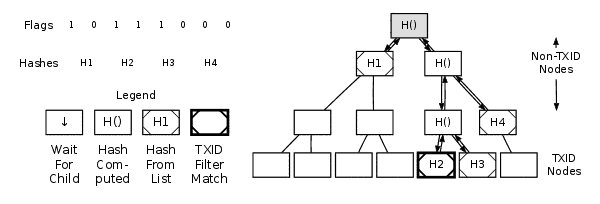
\includegraphics[width=\linewidth]{image/merkleblock-parsing}
	\caption{شکل مثال تحلیل پیام \texttt{merkleblock} در سمت کاربر سبک.\cite{P2P_ref}}
	\label{fig:merkleblock-parsing}
\end{figure}

با توجه به توضیحات بالا، گام‌های محاسبهٔ اثبات مرکل با توجه به پیام \texttt{merkleblock} دریافت شده در مثال به صورت زیر خواهد بود:

\begin{enumerate}
		\item {%
		باتوجه به اینکه تعداد تراکنش‌ها هفت عدد است، یک درخت مرکل سه لایه، مطابق شکل \ref{fig:merkleblock-parsing} ایجاد می‌کنیم که در ابتدا تمام گره‌های آن خالی باشد.
	}
	\item {%
		از ریشهٔ مرکل شروع می‌کنیم. مقدار اولین بیت \lr{flags} یک است. به این ترتیب مقدار گره ریشه بعدا و با توجه به مقدار بچه‌هایش مشخص می‌شود. گره بعدی مورد بررسی را بچهٔ سمت چپ ریشهٔ مرکل قرار می‌دهیم. برای شماره گذاری، گره ریشه را گره شمارهٔ یک می‌نامیم.
	}

	\item {%
در این مرحله، گره مورد بررسی گره بچهٔ سمت چپ ریشهٔ مرکل است. با توجه به اینکه بیت بعدی \lr{flags} برابر صفر است، اولین چکیدهٔ استفاده نشده (\lr{Hash \#1}) را در این گره قرار می‌دهیم و دیگر کاری با گره‌های زیر دستی آن داریم. این گره را گره شمارهٔ دو می‌نامیم. به این ترتیب مطابق شکل \ref{fig:merkleblock-parsing} مقدار \lr{H1} در این گره قرار می‌گیرد. به گره بالاتر (ریشهٔ مرکل) برگشته و بچهٔ راستی آن را انتخاب می‌کنیم.
	}
	\item{%
	شماره این گره را سه می‌گذاریم. مقدار بیت بعدی (سوم) \lr{flags} برابر ۱ است، پس  مقدار این گره باید توسط گره‌های زیردستی آن محاسبه شود. به این ترتیب، بچهٔ سمت چپی آن انتخاب می‌شود. 
}
	\item{%
	شمارهٔ این گره را چهار می‌گذاریم. در این مرحله‌ هم مانند مرحلهٔ قبل، چون بیت چهارم \lr{flags} نیز یک است گره بچهٔ سمت چپی انتخاب می‌شود.
}
	\item{%
	شمارهٔ این گره را پنج می‌نامیم. در این مرحله یک گره \lr{TXID} انتخاب شده است. از آن‌جا که گره‌های مربوط به تراکنش‌ها زیرگره‌ای ندارند، مقدار آن‌ها حتما باید توسط گره کامل در اختیار گره سبک قرار گیرد. به این ترتیب مقدار چکیدهٔ استفاده نشدهٔ بعدی، یعنی \lr{Hash \#2} را در این گره قرار می‌دهیم. مقدار بیت پنجم \lr{flags} که متناظر با این گره است برابر یک بوده که این معنا را می‌رساند که این \lr{TXID} برای تراکنشی است که یکی از عناصر آن با فیلتر بلوم منطبق شده‌اند پس به گره سبک دریافت کننده مربوط است. 
}

	\item{%
	در مرحلهٔ بعدی، به گره پدر (چهارم) برگشته و گره بچهٔ سمت راستی انتخاب می‌شود. این گره، گره ششم است. باز هم چون این گره، بچه‌ای ندارد و مربوط به یک \lr{TXID} است، مقدار  \lr{Hash \#3} را در آن قرار می‌دهیم. بیت ششم \lr{flags} صفر بوده به این معنا است که این تراکنش با فیلتر منطبق نشده است. ارسال آن صرفا برای اثبات مرکل نیاز است.
}

	\item{%
	به گره پدر (گره چهارم) بر می‌گردیم. از آن‌جایی که اطلاعات لازم برای محاسبهٔ چکیدهٔ این گره را از دو مقدار  \lr{TXID} داده شده داریم، مقدار چکیدهٔ را محاسبه کرده و سپس گره بالاتر را انتخاب می‌کنیم. 
}
	\item{%
	در این مرحله وارد بچهٔ راست سومین گره می‌شویم. چون مقدار بیت هفتم \lr{flags} صفر است، چکیدهٔ \lr{Hash \#4} را درون آن قرار می‌دهیم. در این مرحله دیگر گره‌ای نیست که گره کامل مقدار آن را فرستاده باشد و بیت آخر \lr{flags} به خاطر لایی گذاری مقدار صفر دارد. 
}
	\item{%
	در مرحلهٔ آخر مقدار چکیدهٔ گره سوم و به تبع آن مقدار ریشهٔ درخت مرکل را محاسبه می‌کنیم. بررسی می‌شود که مقدار ریشهٔ محاسبه شده با مقدار ریشهٔ مرکلی که در سرایند بلوک قرار داشته است یکسان باشد.
}
\end{enumerate}


\subsubsection{ملاحظات پیاده‌سازی}
بیت‌کوین‌جی\cite{bitcoinj} به صورت پیش‌فرض، نرخ خطای نوع دو را برابر $0.1$ درصد قرار می‌دهد. هرچند که بالا بردن نرخ خطای نوع دو می‌تواند به حفظ بهتر حریم خصوصی کاربران سبک بیانجامد اما نه تنها باعث افزایش پهنای باند مصرفی کاربر سبک می‌شود، بلکه احتمال آن که آدرس‌های پر استفاده‌ای مثل 
ساتوشی‌دایس\LTRfootnote{%
	\lr{Satoshi Dice (\url{https://satoshidice.com/})} - %
سایت ساتوشی‌دایس درحال حاضر تنها از بیت‌کوین‌کش پشتیبانی می‌کند!}،
که یک سایت شرط‌بندی مبتنی بر زنجیرهٔ بلوکی است، منطبق با فیلتر بلوم شود بیشتر خواهد شد. در این صورت اطلاعات به شدت زیادی برای کاربر سبک ارسال خواهد شد و اگر کاربر سبک به گره کامل هم‌گام‌ساز اجازه دهد که فیلتر را به‌روز رسانی کند، به سرعت فیلتر اشباع و بلااستفاده خواهد شد.
 
در کتاب‌خانهٔ بیت‌کوین‌جی، اگر کاربر بخواهد $m$ عنصر را در فیلتر بلوم قرار دهد، مقادیر اندازه فیلتر ($n$) و تعداد توابع چکیده‌ساز آن ($k$) با توجه به $100$ عنصر اضافه‌تر طبق فرمول‌های \eqref{eq:n_of_bloom_filter} و \eqref{eq:k_of_bloom_filter} تعیین می‌شوند 
$M=m+100$ \cite{Gervais2014}.
 هدف از این کار آن است که امکان اضافه شدن عناصر جدید به فیلتر بلوم توسط خود کاربر یا توسط گره کامل، بدون نیاز به به‌روزرسانی آن مطابق آن‌چه قبل‌تر توضیح داده شد، فراهم باشد به نحوی که فیلتر بلوم سریع پر نشود و نرخ خطای نوع دو آن به قدری زیاد نشود که فیلتر بلوم عملا بلااستفاده شود. در حالی که به مرور زمان به تعداد عناصر فیلتر بلوم یک کاربر SPV اضافه می‌شود، قاعدتا، مقادیر $k$ و $n$ تغییری نمی‌کنند. اما اگر کاربر SPV نیاز به راه‌اندازی مجدد کیف‌پولش داشته باشد، در راه‌اندازی دوباره، نرم‌افزار بیت‌کوین‌جی با توجه به $m$، جدید، اقدام به محاسبهٔ $M=m+100$ می‌نماید و به این ترتیب مقادیر  $k$ و $n$ برای فیلتر جدید متفاوت خواهند بود.
 
همچنین در پیاده‌سازی گره سبک بیت‌کوین‌جِی برای هر آدرس، کلید عمومی (\lr{PubKey}) و چکیدهٔ کلید عمومی (\lr{PubKeyHash}) گذاشته می‌شود. پس به ازای یک آدرس بیت‌کوین، دو عنصر در فیلتر بلوم قرار می‌گیرند. به بیان دیگر، در ازای قرار دادن $N$ آدرس در فیلتر بلوم، $m=2N$ عنصر در آن قرار می‌گیرد پس با توجه به آن‌چه در بالا گفته شد، می‌توان نوشت $M=2N+100$. قرار دادن کلید عمومی و چکیدهٔ آن یک آسیب‌پذیری در فیلتر بلوم ایجاد خواهد کرد که به گره متخاصم این امکان را می‌دهد که در صورتی که متوجه شود یک \lr{PubKey} در فیلتر بلوم قرار دارد، مقدار چکیده (\lr{PubKeyHash}) آن  را نیز امتحان می‌کند. اگر مقدار چکیده هم در فیلتر بلوم قرار داشت، با اطمینان بیشتری می‌تواند مطمئن شود که این آدرس، یکی از آدرس‌های کاربر سبکِ استفاده کننده از فیلتر بلوم است. قطعه کد زیر بخشی از پیاده‌سازی فیلتر بلوم در کد بیت‌کوین‌جِی است \cite{bitcoinj_BloomFilter} که این مسئله را به خوبی نشان می‌دهد.


\lr{
	\texttt{/** Inserts the given key and equivalent hashed form (for the address). */\\
		public synchronized void insert(ECKey key) \{\\
		insert(key.getPubKey());\\
		insert(key.getPubKeyHash());\\
		\}\\}
}


در پایان‌نامهٔ\cite{Nick2015}، با هدف پیدا کردن آدرس‌های نهفته شده در این فیلتر بلوم با استفاده از این آسیب‌پذیری، در بازهٔ تاریخی $12$ دسامبر $2014$ الی $10$ فوریه $2015$، یک گره کامل راه‌اندازی شده و شروع به جمع‌آوری $70,078$ فیلتر بلوم از کاربران سبک کرده است. همچنین، در این پایان‌نامه، مجموعه‌ای از تمام کلید عمومی‌ها (\lr{PubKey}) و چکیدهٔ کلید عمومی (\lr{PubKeyHash}) متناظر آن‌ها که در زنجیرهٔ بلوکی مورد استفاده قرار گرفته‌اند جمع‌آوری شده است. در نهایت همهٔ آن‌ها را با تمام فیلتر‌های بلوم جمع شده تطبیق داده است. اگر هر جفت کلید عمومی و چکیدهٔ آن بر فیلتر منطبق بود، نتیجه گرفته است که آن آدرس در آن فیلتر قرار دارد. در نهایت این پایان‌نامه توانسته است به $55,111$ جفتِ کلید عمومی و چکیدهٔ آن برسد که هردو در یک فیلتر بلوم منطبق هستند.

هرچند که این ایراد به نظر ایرادی می‌آید که به سادگی قابل حل شدن باشد، اما در صورتی که بیت‌کوین‌جی کلید عمومی‌ها را در فیلتر قرار ندهد، کیف پول‌هایی که از آن کتاب‌خانه استفاده می‌کنند نخواهند توانست از تراکنش‌هایی که خروجی آن‌ها \lr{P2PK} است مطلع شود. در حالی که، بیت‌کوین‌جی می‌خواهد از تمام انواع تراکنش‌ها پشتیبانی کند. به خاطر همین، باتوجه به آگاهی به وجود این مشکل، اقدامی برای برطرف کردن آن انجام نشده است.

در کنار مشکلات ذکر شده، استفاده از فیلتر بلوم در شبکهٔ همتا‌به‌همتای بیت‌کوین با آسیب‌پذیری‌ها و چالش‌های بیشتری مواجه است که عملا این ابزار را برای حفظ حریم خصوصی کاربران سبک بلااستفاده کرده است. در بخش \ref{Vulnerabilities} به بررسی این ضعف‌ها پرداخته شده است.

\subsubsection{آسیب‌‌پذیری‌ها }
\label{Vulnerabilities}
مقالهٔ \cite{Gervais2014} به طور مفصل به بررسی آسیب‌پذیری‌های موجود در فیلتر بلوم استفاده شده در شبکهٔ همتا‌به‌همتای بیت‌کوین پرداخته است. در این مقاله توضیح داده شده است که فیلتر بلوم نشت اطلاعاتی بسیار زیادی دارد که این نشت به تعداد آدرس‌هایی که یک کاربر دارد وابسته است. اگر کاربر تعداد متوسطی، مثلا $10$ آدرس، را در فیلتر بلومی قرار دهد، مهاجم می‌تواند با احتمال خوبی آدرس‌های قرار گرفته شده در فیلتر بلوم را حدس بزند. به عنوان مثال احتمال درست حدس زدن آدرس‌های فیلتر بلوم با $10$ آدرس برابر $0.99$ است.  

علاوه بر این حتی اگر تعداد آدرس‌ها در فیلتر‌ بلوم افزایش پیدا کند، در حالی که مهاجم بتواند به دو فیلتر بلوم مربوط به یک کاربر سبک دست پیدا کند، قادر خواهد بود که با دقت بالایی آدرس‌های مربوط به کاربر سبک را تشخیص دهد. چرا که اگر یک گره کامل متخاصم دو فیلتر بلوم متفاوت از یک کیف پول را در دست داشته باشد، می‌تواند با وارد کردن عناصر به هر دو فیلتر، تا حد قابل ملاحظه‌ای خطاهای نوع دوم را برطرف نماید\cite{Nick2015}. لازم به ذکر است که در پیاده‌سازی‌های فعلی با راه‌اندازی مجدد گره سبک، چون از مقدار تصادفی \lr{nTweak} متفاوتی استفاده خواهد شد، فیلتر بلوم تغییر می‌کند و به گره کامل متخاصم شانس دسترسی به فیلتری‌های بلوم متعددی از یک کاربر سبک را می‌دهد\cite{Gervais2014} .

در مقالهٔ \cite{Gervais2014}، به معرفی یک معیار برای سنجش حریم خصوصی  فیلتر بلوم پرداخته است. این معیار اینطور تعریف می‌شود که 
$P_{h_{(j)}}$
 برابر است با احتمال آن‌که یک گره متخاصم، ‌$j$ عنصری که واقعا در فیلتر بلوم قرار گرفته‌اند و فرد متخاصم اطلاعاتی در مورد آن‌ها نداشته است را درست حدس بزند. محاسبهٔ $P_{h_{(j)}}$ به صورت زیر است:
%N_v = S
 \begin{equation}
 \label{eq:P_h}
 P_{h_{(j)}} = \prod_{k=0}^{j-1}\frac{N-k}{N+N_v-k} = \frac{N}{N+N_v}\cdot\frac{N-1}{N+N_v-1} \ldots
 \end{equation}
  
  که در آن $N$ تعداد آدرس‌هایی است که در بیت‌کوین قرار داده شده است. از آن‌جایی که هم \lr{PubKey} و هم \lr{PubKeyHash} درون فیلتر بلوم قرار می‌گیرند، تعداد عناصر قرار گرفته در فیلتر بلوم برابر $m=2N$ است. $N_v$ هم تعداد اعضای مجموعه‌ٔ عناصری است که به خاطر خطای نوع دو با فیلتر بلوم منطبق می‌شوند. از نظر شهودی، معادلهٔ \eqref{eq:P_h} به معنی احتمال آن است که $j$ آدرس انتخاب شده از بین تمام آدرس‌هایی که منطبق با فیلتر بلوم می‌شوند، جزء آدرس‌های اصلی فیلتر باشند.
  
   با توجه به معادلهٔ \eqref{eq:P_h} احتمال آن‌که کاربر متخاصم تمام آدرس‌هایی که در حقیقت درون فیلتر بلوم $B$ هستند را به درستی حدس بزند، برابر 
  $P_{h_{(N)}} = \prod_{k=0}^{N-1}\frac{N-k}{N+N_v-k} = \frac{N!N_v!}{(N+N_v)!}$
  خواهد بود\cite{Gervais2014}. بدیهی است که هر چه مقدار $P_{h_{(.)}}$ بیش‌تر باشد،‌ فیلتر بلوم حریم خصوصی را کمتر حفظ می‌کند. علاوه بر این گره کامل می‌تواند تعداد عناصر قرارداده شده در فیلتر را نیز حدس بزند که این خود می‌تواند به برملاء شدن اطلاعات کاربر کمک نماید. در این مقاله با فرض این‌که گره کامل متخاصم تنها بتواند به یک فیلتر بلوم مربوط به یک کیف پول دسترسی پیدا کند، می‌تواند تخمینی از تعداد عناصر موجود در یک فیلتر بلوم را با توجه به اندازهٔ فیلتر، توابع چکیده‌ساز و تعداد بیت‌هایی از فیلتر که یک شده‌اند انجام دهد. این مقاله این تخمین را با بهره‌گیری از ایدهٔ مقالهٔ \cite{Swamidass2007} محاسبه کرده است که به شرح زیر است:
  
   \begin{equation}
  \label{eq:m_estimation}
 m \approx -n\frac{\ln\left(1-\frac{X}{n}\right)}{k}
  \end{equation}
 
 که در آن $X$ تعداد بیت‌های فیلتر بلوم مورد نظر است. از طرف دیگر  اگر 
 $\mathcal{B}_i$
 تمام آدرس‌هایی در شبکهٔ بیت‌کوین باشد که در فیلتر بلوم صدق می‌کنند مقدار آن برابر 
 $|\mathcal{B}_i| = N + N_v$
 خواهد بود. پس:
  \begin{equation}
 \label{eq:N_v_estimation}
 N_v = |\mathcal{B}_i| - N  \approx  |N_u-N|P_f(2N) 
 \end{equation}
 
 که در آن $N_u$ تعداد کل آدرس‌های بیت‌کوین و $P_f(2N)$ احتمال خطای نوع دو فیلتر به ازای قرار دادن $2N$ عنصر در آن است. به این ترتیب می‌توان فرمول \eqref{eq:P_h} را به صورت زیر نوشت:
 
  \begin{equation}
 \label{eq:P_h_estimation}
 P_{h_{(j)}} = \prod_{k=0}^{j-1}\frac{N-k}{N+N_v-k} \approx \prod_{k=0}^{j-1}\frac{N-k}{N+|N_u-N|P_f(2N)-k}
 \end{equation}

که در این معادله $N_u$ تعداد تمام آدرس‌های استفاده شده در شبکهٔ بیت‌کوین بوده که مقدار آن در زمان نگارش این پایان‌نامه $30.4$ میلیون آدرس است\LTRfootnote{\lr{\url{https://rb.gy/3o6nrm}}}.

همان‌طور که قبل‌تر گفته شده بود طبق \cite{Gervais2014} در زمان ساختن ابتدائی فیلتر بلوم در بیت‌کوین‌جی، مقادیر $n$ و $k$ با توجه به $100$ عنصر بیشتر از تعداد عناصری که کاربر می‌خواهد وارد کند انتخاب می‌شوند ($M=m+100$). به این‌ترتیب مقدار $P_f(m)$ بسیار کمتر از حالتی است که تمام $M$ عنصر در فیلتر بلوم قرار گرفته باشد ($P_t = P_f(M)$). شکل \ref{fig:ptvspf} تفاوت $P_t$ و $P_f$ را با توجه به تعداد آدرس‌های قرار گرفته در فیلتر بلوم نشان می‌دهد. 

\begin{figure}
	\centering
	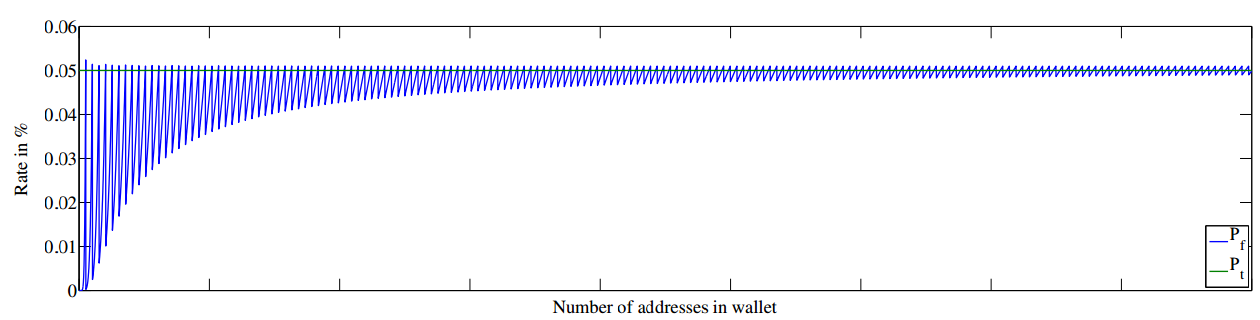
\includegraphics[width=\linewidth]{image/Pt_vs_Pf}
	\caption{
		مقادیر محاسبه شده برای $P_f$ و $P_t$ با توجه به تعداد آدرس‌های ($N$) قرار داده‌شده در فیلتر بلوم. محور افقی این نمودار، نسبت $m$ فعلی فیلتر به $M$ انتخاب شده در زمان راه‌اندازی است.
		\cite{Gervais2014}}
	\label{fig:ptvspf}
\end{figure}

کوچک بودن 
$P_f(2N)$
نسبت به  
$P_t$
باعث می‌شود که امکان فاش شدن آدرس‌های اصلی فیلتر بلوم، در زمان راه‌اندازی فیلتر وقتی تعداد آدرس‌های آن کم باشد، بسیار بالاتر از حد انتظار باشد. به عنوان مثال، در یک فیلتر بلوم با $15$ آدرس و به تبع آن $30$ عنصر، مقدار $M=130$ خواهد بود. در نتیجه، با توجه به فرمول‌های 
\eqref{eq:n_of_bloom_filter}،
\eqref{eq:k_of_bloom_filter} و
\eqref{eq:Pf_of_bloom_filter_Mullin}
 برای نرخ خطای دوی هدف
$P_t=0.001$
 خواهیم داشت:
$n=1869$،
$k=10$ و
$P_f(30)=5.1\times10^{-9}$.

حال با توجه به فرمول \eqref{eq:P_h_estimation} احتمال آن‌که گره کامل متخاصم بتواند  یکی از آدرس‌های قرارگرفته در فیلتر بلوم را حدس بزند برابر 
$P_{h_{(1)}} = 0.99$
خواهد بود. به همین ترتیب گره کامل متخاصم می‌تواند با احتمال
$P_{h_{(15)}} = 0.8$
تمام آدرس‌های اصلی داخل فیلتر بلوم را حدس بزند. جدول \ref{table:P_h} از مقالهٔ \cite{Gervais2014} مقایسه‌ای بین تعداد آدرس‌های قرارگرفته در فیلتر بلوم در زمان راه‌اندازی و احتمال حدس زدن آدرس‌های آن توسط گره متخاصم را نشان داده است. توجه شود که مقادیر
$P_{h_{(.)}}$
نزولی اکید نیستند. از نظر شهودی نیز انتظار می‌رود که هرچه تعداد آدرس‌های یک فیلتر بلوم، در مقایسه با تمام آدرس‌های بیت‌کوین، افزایش پیدا کند، احتمال آن‌که آدرسی که در فیلتر بلوم منطبق است جزء آدرس‌های اصلی آن باشد بیش‌تر می‌شود. این ویژگی در مقادیر 
$P_{h_{(1)}}$
در جدول \ref{table:P_h} قابل مشاهده است. شکل \ref{fig:ph1} نموداری از احتمال حدس درست یک آدرس اصلی فیلتر بلوم با توجه به تعداد آدرس‌های آن در راه‌اندازی اولیه است. 
\begin{figure}
	\centering
	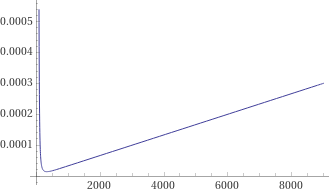
\includegraphics[width=0.7\linewidth]{image/P_h_1}
	\caption{%
		احتمال حدس درست یک آدرس اصلی فیلتر بلوم 
		($P_{h_{(1)}}$)
		با توجه به تعداد آدرس‌های آن ($N$) در راه‌اندازی اولیه.}
	\label{fig:ph1}
\end{figure}


\begin{table}
	
	\caption{%
		مقادیر 
		$P_{h_{(.)}}$
		با توجه به $N$
		($P_t=\%0.1$).
		\cite{Gervais2014}.
	}
	\label{table:P_h}
	\centering
	\begin{tabular}{|c|c|c|c|c|c|}
		\hline 
		\lr{$N$} & \lr{$1$} & \lr{$19$} & \lr{$49$}& \lr{$54$} & \lr{$8,999$}\\
		\hline
		\lr{$P_{h_{(1)}}$} & \lr{$1(\pm0)$} & \lr{$0.42(\pm0.03)$} & \lr{$0.0021(\pm0.00019)$} & \lr{$0.14(\pm0.0059)$} & \lr{$0.21(\pm0.00075)$}\\
		%----
		\lr{$P_{h_{([N/2])}}$} & \lr{$-$} & \lr{$0.000026$} & \lr{$0$} & \lr{$0$} & \lr{$0$}\\
		%----
		\lr{$P_{h_{([N])}}$} & \lr{$1$} & \lr{$0$} & \lr{$0$} & \lr{$0$} & \lr{$0$}\\
		\hline
 		
	\end{tabular}

\end{table}

	
در مقالهٔ \cite{Gervais2014} همچنین اثبات کرده است که اگر یک کاربر سبک دو فیلتر بلوم با اعداد تصادفی (\lr{nTweak}) متفاوت اما با اعضای دارای اشتراک تولید کند، احتمال آن‌که یک گره متخاصم $j$ عنصری که واقعا در فیلتر بلوم قرار دارند حدس بزند به صورت زیر محاسبه می‌شود:
\begin{equation}
\label{eq:P_h_multi_Bloom}
P_{h_{(j)}} \approx \prod_{k=0}^{j-1}\frac{N_1-k}{N_1+P_f(m_1)P_f(m_2)N_u-k}
\end{equation}

که
$P_{h_{(j)}}$
بدست آمده، به طور قابل ملاحظه‌ای، بیشتر از زمانی است که گره متخاصم تنها به یک فیلتر بلوم دسترسی داشته باشد \eqref{eq:P_h}. 

امکان جبران حدودی آسیب‌پذیری‌های گفته شده تا اینجا با اصلاح رفتار کاربر سبک وجود دارد. در قسمت \ref{change_behaviour} مروری بر کارهایی که کاربر سبکی که از بیت‌کوین‌جی استفاده می‌نماید می‌تواند انجام دهد تا بتواند تا حد ممکن آدرس‌هایش را از گره کاملی که از آن خدمات دریافت می‌کند حفظ نماید، انجام شده است. با این حال آسیب‌پذیری‌های دیگری برای این روش وجو دارد که نیاز به توجه بیشتر دارد.

آسیب‌پذیری دیگر آن‌ است که، به صورت کلی، در کاربرد‌های حفظ حریم خصوصی با استفاده از فیلتر بلوم، لازم است که به این مسئله توجه شود که اگر با قرار دادن آدرس $x$ در فیلتر بلوم، تعدادی بیت یک شود آیا هر کدام از این بیت‌ها از طریق قرار دادن یک یا چند عنصر پنهان‌سازی (خطای نوع دو) یک می‌شوند؟ به بیان دیگر اگر $b[i]$ فیلتر بلوم تنها توسط عنصر $x$ یک شود و نتوان آن بیت‌ را با قرار دادن عناصری غیر عضو ولی منطبق با فیلتر بلوم یک نمود، امکان حاشا کردن آنکه x در آدرس‌های مطلوب کاربر سبک قرار دارد، ممکن نخواهد بود. در نتیجه، اگر گره کامل متوجه شود که فقط به ازای یک آدرس $x$ خاص، خروجی توابع چکیده‌ساز به یک یا چند بیت مشخص نگاشت می‌شوند، می‌فهمد که حتما آدرس  $x$ جزء آدرس‌های اصلی قرار گرفته در فیلتر بلوم بوده است و گره سبک نمی‌تواند وجود آن آدرس را «حاشا» کند. مقاله \cite{Bianchi2012} ضمن اشاره به این آسیب‌پذیری، معیاری برای سنجش حریم خصوصی فیلتر بلوم با توجه به احتمال آنکه بیت‌های یک شده در فیلتر بلوم توسط عناصر غیر عضو پوشش داده شوند، ارائه کرده است که در بخش \ref{gamma-deniability} به آن پرداخته شده است.

یک مشکل اساسی دیگر روش استفاده از فیلتر بلوم \cite{Hearn2013}، بار پردازشی بسیار زیاد آن بر روی گره کامل ارائه دهندهٔ این سرویس است چرا که به ازای هر بلوک جدید باید تک‌تک عناصر مهم همهٔ تراکنش‌های بلوک را با تمامی فیلتر‌های بلومی که کاربران سبک با او به اشتراک گذاشته‌اند بررسی کند. هر بار بررسی وجود یک عنصر در یک فیلتر بلوم نیاز به چند مرتبه (حداکثر ۵۰ مرتبه) اجرای توابع چکیده‌ساز را دارد. از این رو گره کامل می‌تواند مورد 
%حملهٔ منع خدمت\RTLfootnote{\lr{Denial of Service Attack}} 
\gls{Denial of Service Attack}
قرار گیرد. کد منبع \cite{PeterTodd} یک کد پیاده‌سازی این حمله به زبان 
%پایتون\RTLfootnote{Python} 
\gls{Python}
است. با این حال تحلیل این آسیب‌پذیری نیاز به توجه بیشتری دارد.

آسیب‌پذیری دیگری که در ارتباط با پرسمان‌ گره سبک از گره کامل وجود دارد، تحلیل بسامد پرسمان یک آدرس  و مقایسهٔ پدیدار شدن آن در زنجیرهٔ بلوکی است. مسئلهٔ دیگر مقایسهٔ بازه‌های زمانی فعالیت یک گره سبک و آدرس‌هایی که در آن زمان در زنجیرهٔ بلوکی قرار گرفته و طبق فیلتر بلوم کاربر برای وی ارسال می‌شود، است. در این پایان‌نامه به صورت خاص بر روی این دو موضوع تمرکز شده است. 

در حال حاضر بسیاری از کاربران سبک بیت‌کوین هستند که جز سرمایه‌گذاری و نگه‌داری طولانی‌مدت بیت‌کوین فعالیت اقتصادی دیگری با آن انجام نمی‌دهند. این کاربران، خواه از کیف‌پول‌های سرد استفاده نمایند خواه نه، احتمال آن که همواره کیف پولشان در حال اجرا و هم‌گام سازی با شبکه باشد بسیار پایین است. در تلفن‌های همراه، به خاطر حفظ طول عمر باتری، در نتیجهٔ استفاده نشدن طولانی مدت از نرم‌افزار کیف پول، فعالیت‌‌های پس‌زمنیه‌‌ای کیف‌پول‌ها متوقف می‌شود.  

هرچند که متاسفانه تا کنون جمع‌آوری اطلاعاتی راجع به زمان‌های فعالیت گره‌های سبک و اتصال آن‌ها به گره‌های کامل انجام نشده است اما همچنان دور از ذهن نیست که فرض کنیم نرم‌افزار کیف پول کاربران کم فعالیت، اکثرا، فقط زمان‌هایی به شبکه متصل می‌شوند که بخواهند از قرارگیری تراکنشِ به تازگی منتشر شدهٔ خود در زنجیرهٔ بلوکی مطلع شوند یا اینکه بررسی کنند که تراکنشی که از طریق دیگری انتظار دریافتش را داشته باشند در زنجیرهٔ بلوکی ثبت شده باشد. 

به این ترتیب اگر فرض کنیم که گره سبک کم فعالیت $l_i$ در هر بار اتصال به یک گره کامل مشخص (مثلا $f_j$) در شبکهٔ بیت‌کوین  متصل شود، و تنها در زمان‌هایی که انتظار ثبت تراکنش مربوط به خودش را داشت، با شبکه همگام شود و در بازهٔ زمانی اطراف آن به پیام‌های \texttt{inv} از طرف گره کامل $f_j$ پاسخ‌ \texttt{getdata} را ارسال نماید، احتمال آن‌که تراکنش‌های منطبق شده با فیلتر بلوم کاربر که برایش ارسال می‌شوند، واقعا مربوط به کاربر سبک باشد، بسیار بیشتر خواهد بود. چرا که در آن بازه، از آن‌جایی که  تعداد تراکنش‌های به نسب کمتری در فیلتر بلوم آزموده می‌شوند،‌ تعداد تراکنش‌های حاصل از خطای نوع دو به نسبت بسیار کم خواهند بود. به این ترتیب گره $f_j$ با احتمال بیشتری می‌تواند مطمئن باشد که تراکنش‌هایی که به کاربری که به تازگی متصل شده است ارسال می‌شوند، مربوط به خودش است.  این آسیب‌پذیری در روش‌های بعدی که در فصل \ref{LitReview} به آن‌ها پرداخته خواهد شود نیز وجود دارد. هرچند در ابتدا فرض اتصال همیشگی به یک گره کامل یکسان ناشدنی به نظر بیاید، اما یک گره کامل متخاصم می‌تواند بدون نیاز به پرداخت هزینه‌ای، با اجرای 
%حملهٔ سیبیل\RTLfootnote{\lr{Sybil Attack}}
\gls{Sybil Attack}
هویت‌های جعلی زیادی در شبکه ایجاد نماید تا شانس ارتباطش با یک گره سبک را در به‌روزرسانی‌های او بالا ببرد. 

حملهٔ دیگری که می‌شود تعریف کرد که نسبت به حملهٔ قبلی شدنی‌تر باشد، آن است که گره کامل، سابقهٔ پرسمان‌های انجام شده از یک کیف پول به خصوص را ذخیره نماید. تشخیص این‌که پرسمان‌های صورت گرفته مربوط به یک کیف پول است می‌تواند از روی فیلتر‌های بلوم یکسانی که ارسال می‌شود تشخیص داده شود. همچنین اگر کاربر سبک فیلتر بلوم خود را عوض نماید اما از آدرس‌های یکسانی در فیلتر بلوم جدید هم استفاده کند،‌ گره کامل می‌تواند با مقایسهٔ آدرس‌های مشترک، به متعلق بودن هر دو فیلتر بلوم به یک کیف پول پی ببرد.

گره کامل متخاصم می‌تواند با تحلیل بسامدی که از یک کیف پول درخواست دریافت کرده است (با همان فرض قبلی که گره‌های سبک کم فعالیت ارتباطشان را به طور مداوم با گره کامل حفظ نمی‌کنند)، و مقایسهٔ آن با بسامد قرار گرفتن آدرس‌های منطبق شده بر فیلتر بلوم در زنجیرهٔ بلوکی، در مورد آدرس‌های اصلی قرار گفته شده در فیلتر بلوم اطلاعات کسب نماید. به عنوان مثال اگر یک کاربر سبک حدودا هر سه ماه یک‌بار به یک گره کامل متصل شود، گره کامل می‌تواند آدرس‌هایی که با فیلتر بلوم وی منطبق شده و روزانه در زنجیرهٔ بلوکی ظاهر شده‌اند را حذف نماید. از طرف دیگر کاربری که درخواست‌های زیادی انجام داده است، احتمال این‌که مالک آدرس‌های پر استفاده از فیلتر بلومش باشد بیشتر است. 

از طرف دیگر در روش فیلتر بلوم، گره کامل می‌تواند به بررسی روابط بین آدرس‌های منطبق شده با روش‌هایی مثل \cite{Meiklejohn2013} در یک فیلتر بلوم بپردازد. به این ترتیب می‌تواند احتمال بدهد که آدرس‌هایی که با فیلتر بلوم منطبق شده‌اند اما با آدرس‌های دیگر ارتباطی ندارند، جزء آدرس‌های پوششی فیلتر بلوم هستند\cite{Gervais2014}.  انتخاب تصادفی آدرس‌های خطای نوع دو می‌تواند شامل مشکلات دیگری نیز باشد، مثلا با توجه به \cite{Gervais2014} از آن‌جایی که فیلتر بلوم تازه در نیمهٔ دوم سال $2011$ معرفی شده است، اگر آدرسی که به عنوان خطای نوع دو با فیلتر بلوم منطبق شود مربوط به زمانی قبل‌تر از آن باشد ($2009$ تا $2011$)، گره کامل می‌تواند آن آدرس‌ها را با احتمال بالایی به عنوان خطای نوع دو فیلتر بلوم حساب نماید.

در این پایان‌نامه قصد داریم روشی را ارائه دهیم که کاربر سبک بتواند به صورت هوشمندانه آدرس‌های نامرتبط با خودش را به نحوی انتخاب نماید که بسامد استفاده از این آدرس‌ها برابر با نرخ استفاده از آدرس خودش باشد. همچنین در این روش کاربر سبک مجبور نخواهد بود که آدرس‌های مربوط به خودش را در یک ساختار دادهٔ واحدی مثل فیلتر بلوم قرار دهد که گره کامل بتواند با بررسی روابط بین آدرس‌های آن و آدرس‌های خطای نوع دو،‌ به آدرس‌های اصلی پی ببرد. بلکه چون گره سبک برای درخواست به روزرسانی هر آدرسش از یک سری مجموعه آدرس‌های پوششی نا مرتبط استفاده می‌کند و بقیهٔ آدرس‌های خودش را در آن‌ها قرار نمی‌دهد، گره کامل نمی‌تواند به ارتباط بین آدرس‌های مربوط به آن کاربر SPV پی ببرد. همچنین گره سبک می‌تواند به سادگی مجموعهٔ آدرس‌های خود را به روزرسانی کند، بدون آن‌که حریم خصوصیش از این بابت نقض شود.  


		% فصول دوم: تعاریف، اصول و مبانی نظری
% !TeX root=../main.tex
\chapter{مروری بر کار‌های انجام شده}
\label{LitReview}
%\thispagestyle{empty} 
\section{مقدمه}

مایک هرن\LTRfootnote{\lr{Mike Hearn}}، نویسندهٔ \lr{BIP37} \cite{Hearn2013}
در پست \cite{Hearn2015} خودش اعلام می‌کند که فیلتر بلوم از امنیت کافی برخوردار نیست. او در این پست به برخی از ایراداتی که در بخش \ref{Vulnerabilities} به آن‌ها اشاره شده، پرداخته است. همچنین مروری بر راه‌حل‌های جایگزین از جمله استفاده از روش‌های 
%بازیابی اطلاعات خصوصی\RTLfootnote{\lr{Private Information Retrieval (PIR)}}
%(PIR)
\gls{Private Information Retrieval (PIR)}
(\lr{PIR})، رمزنگاری ارتباط همتا‌به‌همتا برای جلو گیری از افشا شدن اطلاعات نزد طرف‌های متخاصم، از جمله سازمان‌های اطلاعاتی، اشاره می‌کند. هرن همچنین توضیح می‌دهد که حل این مسئله ساده نخواهد بود و به دشواری‌ها و چالش‌های آن اشاره کرده است\cite{Hearn2015}.

علاوه بر این، افراد دیگری پیشنهاد‌های زیادی در تغییر شیوهٔ موجود ارائه کرده‌اند که در این قسمت به بررسی پیشنهاد‌ها و راه‌حل‌هایی که تا کنون برای بهبود حریم خصوصی کاربران سبک منتشر است پرداخته می‌شود. 


\section{
اصلاح رفتار کاربر سبک فعلی جهت حفظ حریم خصوصیش
}
\label{change_behaviour}
در مقالهٔ \cite{Gervais2014} در کنار تحلیل امنیت و بیان ضعف‌های استفاده از فیلتر بلوم در ارتباط بین گره سبک با گره کامل \cite{Hearn2013}، به بیان چند رویه پرداخته است که اگر گره سبک از این رویه‌ها پیروی کند، می‌تواند در عین این که از پروتکل فعلی استفاده می‌کند، تا حدی حریم خصوصی خودش را حفظ کند. در ادامه به بیان این موارد پرداخته می‌شود.

	همان‌طور که در \ref{Vulnerabilities} نشان داده شد، نرخ خطای نوع دوی فیلتر بلوم به طور قابل ملاحظه‌ای تحت تاثیر تعداد عناصر قرار گرفته در یک فیلتر بلوم است. همچنین باید از ایجاد چند فیلتر بلوم با عناصر مشترک پرهیز شود. در نتیجه پیشنهاد می‌شود هر گره سبک در ابتدا یک فیلتر بلوم با $N$ آدرس ایجاد کند به طوری که $M=N$. به این ترتیب، فیلتر بلوم با نرخ خطای نوع دوی هدف، $P_t$، ساخته می‌شود. همچنین پیشنهاد شده است که $M=m$، به این معنی که تنها یکی از مقادیر \lr{PubKey} یا \lr{PubKeyHash} در فیلتر بلوم قرار بگیرد. مقالهٔ \cite{Gervais2014} بررسی کرده است که برای تقریبا $99\%$ از آدرس‌های بیت‌کوین قرار دادن یکی از این دو مقدار در فیلتر بلوم کفایت می‌کند تا تمام تراکنش‌های مرتبط  با خودشان را دریافت نمایند.
	
	گره سبک می‌تواند به مرور که به آدرس‌های بیشتری نیاز پیدا کرد، از $N$ آدرسی که پیش‌پیش در فیلتر بلوم قرار گرفته است، استفاده نماید. زمانی که از تمام این $N$ آدرس استفاده کرد، یک فیلتر بلوم جدید تولید نماید که این هم شامل $N$ آدرس جدید باشد و آدرس مشترکی با فیلتر بلوم قبلی نداشته باشد. گره سبک می‌تواند این که هر آدرسش در کدام فیلتر بلوم قرار گرفته‌ است را تحت اطلاعاتی جانبی، در کنار آدرس‌هایش، ذخیره نماید. در این صورت گره متخاصم نمی‌تواند با در دست داشتن فیلتر‌های بلوم مربوط به یک کیف پول به اطلاعات اضافه‌ای دست پیدا کند. به این ترتیب گره سبک باید همزمان از چند فیلتر بلوم استفاده نماید و آن‌ها را برای گره‌های مختلف ارسال کند. البته خود مقالهٔ \cite{Gervais2014} اذعان داشته است که در صورتی که گره سبک برای اولین بار از یک آدرس از پیش ذخیره شده در فیلتر بلوم استفاده نماید، از آن‌جایی که این آدرس تا الان در زنجیره بلوکی استفاده نشده است و در اولین استفاده‌اش با فیلتر بلوم این کاربر منطبق شده است، می‌تواند گره کامل را مطمئن سازد که این آدرس جزء آدرس‌های اصلی این فیلتر بلوم است.
	
	برای حفظ بیشتر حریم خصوصی کاربر و رفع ضعف ذکر شده، مقالهٔ \cite{Gervais2014} پیشنهاد داده است که گره سبک با توجه به آدرس‌های موجود در زنجیرهٔ بلوکی، که مربوط به خودش نیستند، دست به ایجاد یک فیلتر بلوم بزند. سپس سعی کند برای هر آدرسی که احتیاج دارد، با تلاش‌ها و آزمون‌ و خطا‌های مکرر آدرس جدید را طوری ایجاد نماید که در فیلتر بلوم تولید شده قرار گیرد. در نتیجه در صورت قرار گرفتن آدرس تازه ساخته شدهٔ این گره در زنجیرهٔ بلوکی، احتمال بیشتری وجود خواهد داشت که گره کامل آن تراکنش آن را برای گره‌های دیگری نیز ارسال نماید. اما این روش بار پردازشی زیادی را بر روی گره سبک بابت تولید آدرس جدید تحمیل می‌کند.  
	
در هر بار راه‌اندازی یک کیف پول در یک گره سبک، نرم‌افزار کیف پول شروع به محاسبهٔ مجدد فیلتر بلوم با استفاده از آدرس‌هایش می‌نماید؛ چرا که فیلتر بلوم تولید شده‌اش را در حافظه دائمی ذخیره نمی‌کند. در نتیجه، این موضوع می‌تواند باعث شود که فیلتر‌های بلوم متعددی با $nTweak$های متفاوت اما عناصر یکسان در دست یک گره کامل بیافتد. مقالهٔ \cite{Gervais2014} پیشنهاد داده است که گره سبک فیلتر بلومش و اطلاعات جانبی آن مانند آدرس‌هایی که در آن قرار گرفته است و غیره را در یک حافظهٔ دائمی ذخیره کند. این مقاله تخمین زده است که هر گره سبک نیاز خواهد داشت که برای هر فیلتر بلوم، چیزی در حدود $220$ بایت ذخیره نماید که سربار قابل توجهی به نرم‌افزار کیف پول اضافه نمی‌کند.
	
	روش‌های پیشنهاد شده در این قسمت، هر چند تا حدودی توانسته بودند ضعف‌های اساسی \cite{Hearn2013} را جبران نمایند، اما به طور کامل نتوانسته بودند که ایرادات آن را برطرف کنند.  علاوه بر این، روش‌های پیشنهاد شده نسبت به حملهٔ تحلیل بسامد پرسمان و استفاده، آسیب پذیر است. همچنین راه حل مشخصی  پیشنهاد نشده است که جلوی گره کامل متخاصم گرفته شود تا نتواند از روی روابط بین آدرس‌های یک فیلتر بلوم به آدرس‌های اصلی پی ببرد. باید به این نکته نیز توجه کرد که یکی از دلایلی که در پیاده‌سازی گره سبک، المان‌های فیلتر تازه ساخته شده باتوجه به $M=m+100$ بوده است آن است که اجازهٔ به روزرسانی فیلتر با توجه به تراکنش‌های منتشر شده در شبکه، طبق جدول \ref{table:filterloadMessage}، به گره کامل داده شود و در عین حال جلوی اشباع زودهنگام فیلتر گرفته شود. اما با توجه به راه حل \cite{Gervais2014}، که پیشنهاد داده است که در همان ابتدا $M=m$ باشد، امکان به روزرسانی فیلتر با توجه به تراکنش‌های جدید سلب می‌شود.


\section{معیار 
	حاشاپذیری-$\gamma$ برای
	سنجش حریم خصوصی فیلتر بلوم}
\label{gamma-deniability}

در مقاله \cite{Bianchi2012} معیاری کمّی، بر اساس مدل گمنامی-$K$ 
\cite{Sweeney2002}،
برای اندازه‌گیری حریم خصوصی فیلتر بلوم معرفی شده است.این معیار
\gls{Deniability}-$\gamma$
نام دارد. در این مقاله بیان شده است که احتمال خطای نوع دو ($P_f$) به تنهایی معیار مناسبی برای سنجش حریم خصوصی فیلتر بلوم نیست. بلکه باید تعداد عناصر خطای نوع دو ($N_v$) مورد بررسی قرار گیرد. واضح است که اندازهٔ $N_v$ علاوه بر $P_f$ وابسته به تعداد کل عناصر ($N_u$) است:
$N_v=(N_u-m)\times P_f$.
با توجه به این موضوع، مقاله \cite{Bianchi2012} با بهره‌برداری از نسخهٔ احتمالاتیِ مدل گمنامی-$K$
\cite{Lodha2008}،
یک معیار سنجش گم‌نامی مناسب فیلتر بلوم ارائه داده است. عنوان این معیار «حاشاپذیری-$\gamma$» است. 

در فیلتر بلوم، داده به صورت تجزیه ناپذیر ذخیره می‌شود و در گمنامی-$K$ داده به صورت ساختاریافته و دارای ویژگی‌های مشخصی هست. اما می‌توان شباهت‌های نزدیکی بین آن‌ها در نظر گرفت. به طور شهودی می‌توان این گونه تعبیر کرد که بیت‌های فیلتر ($b[i]$ و $i\in[0,n-1]$) «ویژگی‌های» عنصر $x$ هستند. یعنی، عنصر $x$ دارای ویژگی $b[i]$ است، اگر و تنها اگر به ازای حداقل یک 
$j\in[1,k]$ داشته باشیم 
$H_j(x)=i$.
به این ترتیب می‌توانیم از تعریف گمنامی-$K$ در فیلتر بلوم استفاده نماییم. عنصر $x$، قرار گرفته در فیلتر، گمنام-$K$ یقینی است اگر به ازای تمام بیت‌های $b[i]$  که توسط این عنصر یک شده‌اند، حداقل $K-1$ عنصر خطای نوع دو وجود داشته باشد که به همان بیت‌ها نگاشت شوند.

می‌توان از این تعریف فهمید که برقراری شرایط گمنامی-$K$ یقینی همیشه امکان‌پذیر نیست. از این رو، استفاده از تعمیم احتمالاتی گمنامی-$K$ 
\cite{Lodha2008} 
برای فیلتر بلوم مناسب‌تر است. به این ترتیب مقالهٔ \cite{Bianchi2012} برای عنصری که به فیلتر بلوم اضافه شده است، از صفت «حاشاپذیر» استفاده کرده است.  به این معنی که آیا دارنده فیلتر می‌تواند وجود آن عنصر در فیلتر را انکار نماید یا خیر. به این ترتیب می‌گوییم عنصر $x\in \mathcal{S}$ حاشاپذیر است اگر به ازای 
$\forall i \in \{1..k\}$،
حداقل یک عنصر از مجموعه پنهان‌سازی $v\in \mathcal{V}$ (خطای نوع دو) وجود داشته باشد به گونه‌ای که 
$\exists j \in \{1..k\}$
به شرطی که 
$H_i(x) = H_j(v)$.
به بیان ساده‌تر یک عنصر حاشا‌پذیر است اگر بتوان بدون تغییر بیت‌های فیلتر، آن عنصر را توسط عناصری که عضو فیلتر نیستند جایگذاری کرد. 

فیلتر بلوم $B$، حاشاپذیر-$\gamma$ است (یا دارای ویژگی حاشاپذیری-$\gamma$) است، هر گاه یک عنصر تصادفی آن $x\in \mathcal{S}$ با احتمال $\gamma$ حاشاپذیر باشد. احتمال تقریبی حاشاپذیری-$\gamma$ فیلتر $B$ به صورت معادله \eqref{eq:gamma-deniability} محاسبه می‌شود  \cite{Bianchi2012}.

\begin{equation}
\gamma \left(B\right) \approx \left(1-exp\left(-\frac{N_vk}{n\left(1-e^{-km/n}\right)}\right)\right)^k
\label{eq:gamma-deniability}
\end{equation}

که در آن 
$N_v=(N_u-m)\times P_f$.
هرچه مقدار $\gamma$ به یک نزدیک‌تر باشد، سطح بهتری از حریم خصوصی مُهیا شده است.
شکل \ref{fig:gamma_deniability} مثالی را نشان می‌دهد که در آن   
$\mathcal{S} = \{x_1, x_2, x_3\}$ 
مجموعه عضو فیلتر بلوم است. مجموعهٔ پنهان‌سازی (خطای نوع دو)، شامل عناصر 
$\mathcal{V} = \{v_1, v_2, v_3\}$
می‌شود. عنصر $x_1$ حاشا‌پذیر است چرا که بیت‌های مرتبط با آن، یعنی $b[0]$، $b[2]$ و $b[7]$، توسط عناصر $v_1$ و $v_2$ پوشانده شده است. به همین ترتیب می‌توان نشان داد که عنصر $x_2$ نیز حاشا‌پذیر است. اما عنصر $x_3$ حاشا‌پذیر نیست. چرا که بیت $b[8]$ توسط هیچ‌کدام از عناصر مجموعهٔ پنهان‌سازی پوشانده نشده است. به این ترتیب، این فیلتر به صورت کلی، حاشاپذیر-$0.66$ است.


\begin{figure}
	\centering
	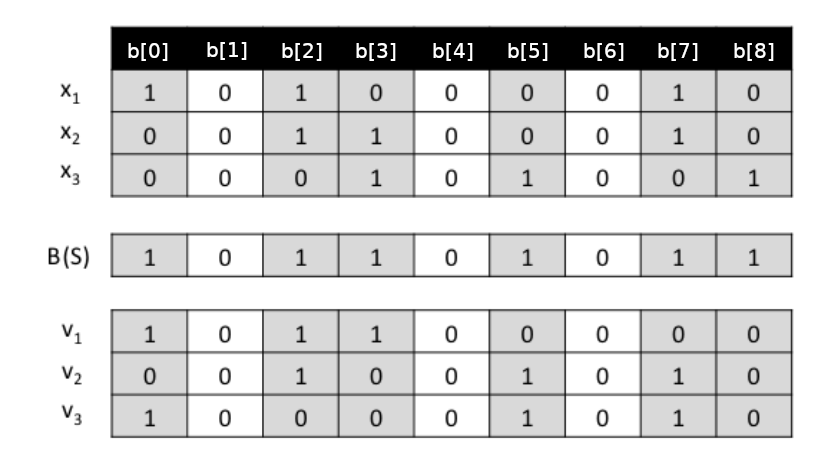
\includegraphics[width=0.8\linewidth]{image/gamma_deniability}
	\caption[مثالی از حاشاپذیری-$\gamma$]{
		یک فیلتر بلوم تشکیل شده از عناصر $\{x_1, x_2, x_3\}$ که سه عنصر $\{v_1, v_2, v_3\}$ را به عنوان خطای نوع دو می‌پذیرد\cite{Bianchi2012}.
		
	}
	\label{fig:gamma_deniability}
\end{figure}

در \cite{Kanemura2017} پیشنهاد شده است که فیلتر بلوم استفاده شده در پروتکل بیت‌کوین با توجه به معیار حاشاپذیری-$\gamma$  
\cite{Bianchi2012}،
ساخته شود. زیرا نرخ خطای نوع دو ($P_t$) به تنهایی برای سنجش حریم خصوصی فیلتر بلوم ساخته شده کافی نیست. به این ترتیب لازم است که طبق معادله \eqref{eq:gamma-deniability} در هر لحظه باتوجه به تعداد آدرس‌های یکتایی که از نقطه بررسی تا آخرین بلوک استخراج شده در زنجیره بلوکی نمایان شده‌اند ($N_u$) و $\gamma$، مقدار $P_t$ تعیین گردد. از آن‌جایی که محاسبه $N_u$ برای گره سبک غیرممکن است، در \cite{Kanemura2017} پیشنهاد شده است که از تکنیک رگرسیون خطی برای تخمین  $N_u$  استفاده شود. ضرایب مدل رگرسیون خطی، باید بصورت متناوب (مثلا به صورت هفتگی) محاسبه گردد. این محاسبه می‌تواند به توسعه دهندگان نرم‌افزار که طرح ارائه شده در \cite{Kanemura2017}  را پیاده‌سازی می‌کنند، سپرده شود. به این ترتیب گره سبک می‌تواند مقدار $P_t$ را به نحوی تعیین کند که از امنیت فیلتر بلوم مطمئن گردد.

روش ارائه شده در \cite{Kanemura2017} دارای اشکالاتی است. یکی از اصلی‌ترین این اشکالات به روزرسانی متناوب فیلتر بلوم باتوجه به تخمین حاصل از $N_u$  است. طبق مقاله \cite{Gervais2014}، اگر گره کامل متخاصم به دو فیتلر بلوم که مربوط به یک گره سبک هستند دست پیدا کند، می‌تواند با دقت بیش‌تری آدرس‌های مربوط به گره سبک را حدس بزند. از این رو تولید متناوب فیلتر بلوم می‌تواند حریم خصوصی کاربر سبک را به خطر بیاندازد.
از ایرادات دیگر این روش می‌توان به افزایش $P_t$ در نتیجهٔ به کار گیری از این طرح اشاره نمود. به این ترتیب، پهنای باند مورد نیاز زیادتر می‌شود. 

\section{فیلترکردن بلوک}
\label{BIP157}
در \cite{Osuntokun2017} پیشنهاد شده است که بر خلاف آن‌که گره سبک فیلتر بلوم را تولید کند و برای گره کامل ارسال نماید، گره کامل یک فیلتر از روی تمام دادگان یک بلوک ایجاد ‌کند. گره سبک به ازای هر بلوک جدید، فیلتر مربوطه را از گره کامل دریافت کرده و خودش بررسی می‌کند که آیا داده مورد نظرش در آن قرار دارد یا نه. اگر داده مورد نظر گره سبک در آن فیلتر قرار داشت، تمام بلوک را از گره کامل دریافت می‌کند. این ایده برای اولین بار در ایمیل آدام بک\LTRfootnote{\lr{Adam Back}}، از دانشمندان حوزهٔ بیت‌کوین، بیان شده است\cite{Back2015}. به فیلتر استفاده شده در این روش 
%فیلتر بلوک\RTLfootnote{\lr{Block Filter}}
\gls{Block Filter}
 گفته می‌شود. کیف پول 
 نوترینو\LTRfootnote{Neutrino}
در حال حاضر از این روش پشتیبانی می‌کند.

از آن‌جایی که مقدار ساخته شده برای فیلتر‌ها یقینی هستند، نیاز است تنها یک مرتبه ساخته شده و ذخیره شوند. بر خلاف فیلتر بلوم، در این روش از یک عدد تصادفی برای ساخت فیلتر استفاده نمی‌شود. از این رو گره کامل از خطر حملات منع خدمت در امان است. در این روش برای هر فیلتر بلوک یک سرایند مرتبط وجود دارد که اندازهٔ این سرایند $32$ بایت بوده و سرایند شامل چکیدهٔ مقدار حاصل از 
%الحاق\RTLfootnote{Concatenate} 
\gls{Concatenate}
چکیدهٔ فیلتر بلوک و سرایند فیلتر بلوک قبلی است. سرایند فیلتر بلوک برای هر بلوک زنجیرهٔ قالبی می‌تواند به عنوان یک خروجی \lr{\texttt{OP\_RETURN}} در تراکنش کوین‌بِیس\LTRfootnote{ \lr{Coinbase}} قرار بگیرد. 

در این روش، هر فیلتر بلوک به ازای هر تراکنش‌ بلوک شامل نبشتهٔ‌های خروجی قبلی که در هر ورودی‌ آن خرج شده است می‌شود همچنین تمام \lr{scriptPubKey}های هر خروجی تمام تراکنش‌ها نیز در آن قرار می‌گیرد. در این روش نیز اگر عنصری در فیلتر قرار گرفته باشد، با احتمال 1 در آن صدق می‌کند اگر قرار نداشته باشد با احتمال $\frac{1}{M}$ با آن منطبق می‌شود. مراحل ساخت فیلتر بلوک با \lr{N} عضو، به شرح زیر است (توجه شود که
$N,M < 2^{32}$)
\begin{enumerate}
	\item {%
	چکیدهٔ تمام اعضای فیلتر بلوک با استفاده از تابع چکیده‌ساز \lr{SipHash} محاسبه می‌شود. سپس خروجی تابع چکیده‌ساز به صورت یکنواخت در بازهٔ 
	$[0, N\times M)$
	نگاشت می‌شود. 
}

\item {%
	مقادیر خروجی مرحلهٔ قبل با توجه به مقدارشان مرتب می‌شوند و اختلاف هر دو مقدار متوالی محاسبه می‌شود. برای کوچک‌ترین مقدار، اختلاف آن با صفر محاسبه می‌شود که برابر با خودش است.
 }

\item {%
مقادیر اختلاف‌ها که از مرحلهٔ قبل بدست آمده پشت سر هم نوشته می‌شوند و به وسیلهٔ 
%کدگذاری گلومب-رایس\RTLfootnote{\lr{Golomb-Rice coding}} 
\gls{Golomb-Rice Coding}
فشرده می‌شوند.
}

\end{enumerate}

از آن‌جا که خروجی مرحلهٔ یک دارای یک 
%توزیع یکنواخت\RTLfootnote{\lr{Uniform distribution}} 
\gls{Uniform Distribution}
است،‌ اختلاف آن‌ها دارای یک 
%توزیع هندسی\RTLfootnote{\lr{Geometric distribution}} 
\gls{Geometric Distribution}
خواهد بود. روش کدگذاری گلومب-رایس در فشرده‌سازی داده‌هایی با توزیع هندسی بهینه عمل می‌کند\cite{Osuntokun2-2017}. برای کدگذاری گلومب-رایس، پارامتر $P$ تعریف می‌شود که طول کد باقیمانده را تعیین می‌کند. این کد‌گذاری به این صورت است که هر مقداری (در اینجا اختلاف بین دو چکیده) بر $2^P$ تقسیم شده و خروجی آن دو قسمت خارج قسمت $q$ و باقیماندهٔ $r$ خواهد بود. سپس، $q$ با روش 
%کدگذاری یگانی\RTLfootnote{\lr{Unary coding}}،
\gls{Unary Coding}
 که به صورت رشته‌ای خواهد بود که با تعداد $q$ یک به همراه یک $0$ نوشته می‌شود. مقدار $r$ هم در $P$ بیت با استاندارد اندین بزرگ نوشته می‌شود. به عنوان مثال کدگذاری عدد $9$ با $P=2$  به صورت
 \lr{\texttt{110 01}} 
 خواهد بود. که در آن $q=2$ و $r=1$ است.
 
 در این روش امکان استفاده از فیلتر‌های مختلف وجود دارد اما در فیلتر اولیهٔ این روش، مقدار $M=784931$ و مقدار $P=19$ است. حال در این پایان‌نامه، برای آن‌که تخمینی از سربار پهنای باندی برای گره سبک در این روش داشته باشیم، به این ترتیب عمل می‌کنیم:
 \begin{itemize}
 	\item {%
 در زمان نگارش این پایان‌نامه، تعداد روزانهٔ هرکدام از ورودی‌ها و خروجی‌های \lr{P2PKH} حدودا برابر $350,000$ عدد است\LTRfootnote{\lr{\url{https://transactionfee.info/charts/inputs-and-outputs-p2pkh/}}} که در مجموع می‌شود $700,000$ عدد در روز. همچنین برای \lr{P2SH}، تعداد خروجی‌ها برابر $310,000$ و تعداد ورودی‌ها برابر $22,000$عدد است\LTRfootnote{\lr{\url{https://transactionfee.info/charts/inputs-and-outputs-p2sh/}}}
 که در مجموع تعداد آن برابر $332,000$ عدد در روز خواهد بود.
به این ترتیب برای هر هر فیلتر بلوک در زمان نگارش پایان‌نامه می‌توان $7167$ عضو متصور شد($N=7167$)
}
\item{%
با فرض اینکه از فیلتر اولیه استفاده شود، $M=784931$ و $P=19$ خواهد بود. به این ترتیب از آن‌‌جا که خروجی چکیدهٔ اعضای فیلتر بلوک، در بازهٔ 
$[0, N\times M)$
نگاشت می‌شوند، نتایج در بازهٔ صفر تا 
$N\times M = 5,625,600,477$
به صورت یکنواخت توزیع خواهد شد.\\
\begin{equation}
\label{eq:Items_in_block_filter}
0\le h_1 \leq h_2 \leq \dots \leq h_N < 5.625 \times 10^{9}
\end{equation}
که در آن $h_i$ها خروجی تابع چکیده‌ساز بعد از نگاشت به بازهٔ گفته شده بوده که به ترتیب اندازهٔ آن‌ها مرتب شده‌اند.
}
\item{%
با توجه به روش گفته شده تفاضل بین $h_i$ها را به صورت زیر محاسبه می‌کنیم:
\begin{equation}
\label{eq:delta_value_in_block_filter}
\delta_i = h_i - h_{i-1}, \ \  1<i\leq N; \quad \delta_1 = h_1
\end{equation}
}
\item{%
حال باید بر روی مقادیر $ \delta_i $ کدگذاری گلومب-رایس اعمال شود و بیت‌های حاصل به ترتیب در کنار هم قرار بگیرند. تعداد بیت‌های خروجی برای یک فیلتر بلوک ($L$) از فرمول زیر محاسبه می‌شود.



\begin{multline}
\label{eq:size_in_block_filter}
L = \sum_{i=1}^{N} \left(\left[\frac{\delta_i}{2^P}\right] + P + 1\right) < \\
\left[\frac{\sum_{i=1}^{N} \delta_i }{2^P}\right] + NP + N  <
\left[\frac{ MN }{2^P}\right] + N(P + 1) 
\end{multline}

که در آن 
$\frac{\delta_i}{2^P}$
تعداد یک‌های حاصل از کدگذاری هر کدام از 
$\delta_i$ها
است و به ازای هر کدام از آن‌ها یک بیت صفر و $P$ بیت شامل باقیمانده قرار داده می‌شود. مجموع تفاضل‌های $ \delta_i $ برابر با $h_N$ می‌شود و با توجه به \eqref{eq:Items_in_block_filter}، این مقدار می‌تواند حداکثر $MN$ باشد.

}
%\item{%
%با توجه به معادلهٔ \eqref{eq:Items_in_block_filter}، و اینکه $h_i$ها توزیع یکنواخت دارند. می‌خواهیم $E\{L\}$ را محاسبه کنیم. 
%\begin{equation}
%\label{eq:E_L_1_block_filter}
%E\{L\} \approx \left[\frac{E\{h_N\}}{2^P}\right] + NP + N
%\end{equation}
%
%که با توجه به \eqref{eq:Items_in_block_filter} و استقلال $h_i$ها ، برای محاسبهٔ $E\{h_N\}$ داریم:
%\begin{equation}
%\label{eq:E_h_N_1_block_filter}
%F_{h_N}(x) = \left[F_{h}(x)\right]^N
%\end{equation}
%
%و از آن‌جایی که توزیع $h$ یکنواخت در بازهٔ 
%$[0, NM)$
%است، خواهیم داشت:
%\begin{align}
%\label{eq:E_h_block_filter}
%F_{h}(x) = \frac{x}{N M} \qquad \text{for} \quad  0 \leq x < NM\\
%\Rightarrow F_{h_N}(x) = \frac{x^N}{(NM)^N} \qquad \text{for} \quad  0 \leq x < NM\\
%\Rightarrow f_{h_N}(x) = \frac{Nx^{N-1}}{(NM)^N} \qquad \text{for} \quad  0 \leq x < NM
%\end{align}
%
%به این ترتیب:
%
%\begin{multline}
%\label{E_h_2_block_filter}
%E\{h_N\} = \int_{0}^{NM} xf_{h_N}(x) dx \\
%= \int_{0}^{NM} \frac{Nx^{N}}{(NM)^N} = \frac{N}{(NM)^N} \cdot \left. \frac{x^{N+1}}{N+1} \right|_0^{NM} = \frac{N^2M}{N+1} \approx NM
%\end{multline}
%
% 
%که با توجه به معادلهٔ بالا و \eqref{eq:E_L_1_block_filter} داریم:
%\begin{equation}
%\label{E_L_2_block_filter}
%E\{L\} \approx \left[\frac{NM}{2^P}\right] + (N+1)P
%\end{equation}
%با توجه به مقادیر $N$، $M$ و $P$ داریم:
%
%\begin{equation}
%\label{E_L_3_block_filter}
%E\{L\} \approx \left[\frac{5.625 \times 10^{9}}{2^{19}}\right] + 7168 \times 19 = 146921\text{b} = 18366\text{B} = 18\text{KB}
%\end{equation}
%
%
%}

\item{%
با توجه به مقادیر $N$، $M$ و $P$ داریم:

\begin{equation}
\label{E_L_3_block_filter}
L < \left[\frac{5.625 \times 10^{9}}{2^{19}}\right] + 7168 \times 19 = 146921\text{b} = 18366\text{B} = 18\text{KB}
\end{equation}


}
 \end{itemize}

به این ترتیب می‌توان گفت که اندازهٔ هر فیلتر بلوک از $18$ کیلوبایت کوچک‌تر است. با توجه به زیاد بودن اندازهٔ $M$، احتمال آن‌که یک بلوک به عنوان خطای نوع دو انتخاب شود بسیار کم خواهد بود. هرچند که کم بودن نرخ خطای نوع دو باعث کاهش پهنای باند مصرفی گره سبک می‌گردد، اما از طرف دیگر می‌تواند حریم خصوصی کاربر سبک را با خطر مواجه کند.

اگر گره سبک از آدرس‌های محدودی استفاده کند به گره کامل متخاصم این امکان را می‌دهد که بتواند با در نظر گرفتن آدرس‌های مشترک بین بلوک‌های درخواست شده توسط آن کاربر، آدرس کاربر را در مجموعه محدود‌تری جست‌وجو نماید. گره کامل با استفاده از گراف تراکنش‌ها حتی می‌تواند به نتایج دقیق‌تری دست پیدا کند\cite{blockfilter-wiki}.

مشکل دیگر این روش، کاربرد آن برای گره‌های سبکی است که تراکنش‌های نسبتا زیادی در شبکه ارسال می‌کنند. حریم خصوصی این گره‌ها نه تنها بیش‌تر در معرض نقض شدن قرار دارد، بلکه، آن‌ها برای هم‌گام سازی با شبکه نیاز است که پهنای باند زیادی را مصرف نمایند. چرا که لازم است برای هر تراکنش، یک بلوک کامل را دانلود نمایند.

گره کامل متخاصم می‌تواند با تحلیل‌ بسامد درخواست‌ها و آدرس‌های بلوک درخواست داده شده تعدادی از آدرس‌های پوششی بلوک‌های درخواست داده شده را کنار بگذارد و در مجموعهٔ کوچک‌تری به جست‌و‌جوی آدرس‌‌های کاربر سبک بپردازد.

\section{بازیابی اطلاعات خصوصی}
\label{PIR}
در مقاله \cite{Qin2019} از روش بازیابی اطلاعات خصوصی (PIR) جهت دریافت اطلاعات تراکنش‌ها از گره‌ کامل استفاده کرده است. بازیابی اطلاعات خصوصی به کاربران این امکان را می‌دهد که از یک پایگاه داده یا مجموعه‌ای از آن‌ها یک پرسمان انجام دهند، به گونه‌ای که سرور پایگاه داده نتواند اطلاعاتی راجع ‌به کاربران درخواست دهنده و درخواست آن‌ها کسب نماید. در مقاله \cite{Qin2019}  از ترکیبی از دو رده بازیابی اطلاعات خصوصی، یعنی بازیابی اطلاعات خصوصی نظریه اطلاعاتی (IT-PIR) و محاسباتی (C-PIR) استفاده کرده است. این ترکیب در مقاله \cite{Devet2014} معرفی شده است. در ،C-PIR  پرسمان توسط کاربر به نحوی کدگذاری می‌شود که پایگاه داده پاسخ مناسب را در اختیار کاربر قرار دهد، اما چیزی از پرسمان و اطلاعات ذخیره شده متوجه نشود. تضمین این حریم خصوصی بر مبنای این فرض است که با اختیار داشتن توان پردازشی محدود، حل برخی مسئله‌ها  غیر ممکن یا سخت خواهد بود \cite{Devet2014}.

رده IT-PIR وابسته به فرض سخت بودن حل الگوریتم‌های پایه رمز نگاری با منابع محاسباتی محدود نیست. پروتکل‌های رده IT-PIR از چند سرور به صورت همزمان استفاده می‌کند. تا زمانی که سرورهایی که تبانی نمی‌کنند از یک تعدادی بیش‌تر باشد، حریم خصوصی کاربر تضمین می‌شود \cite{Devet2014}. 

یکی از نقص‌های IT-PIR آن است که در عمل راه حلی وجود ندارد که بتوان حداقل تعداد سرورهایی که تبانی نکنند را تامین کرد. به ویژه که یک سرور می‌تواند در شبکه 
%حمله سیبیل\RTLfootnote{\lr{Sybil attack}}
\gls{Sybil attack}
را انجام دهد. از طرف دیگر یکی از نقص‌های اساسی C-PIR آن است که به خاطر آن‌که تنها وابسته به یک سرور است، امکان تشخیص پاسخ‌های ناقص یا غیر صحیح از طرف سرور پایگاه داده وجود ندارد \cite{Qin2019}. به بیان ساده‌تر، در کاربرد فعلی سروری که قرار است اطلاعات مربوط به زنجیره بلوکی را در اختیار کاربران سبک قرار دهد،‌ می‌تواند از انشعابی نامعتبر از زنجیره بلوکی استفاده نماید. چون گره سبک با گره‌های کامل دیگر ارتباط ندارد، نمی‌تواند متوجه این مشکل شود.

مقاله \cite{Qin2019} با استفاده از از روشی که در \cite{Devet2014} معرفی شده، از هر دوی  IT-PIR و  C-PIR استفاده کرده است. از این طریق به نقاط قوت هر دو روش دست پیدا کرده و تا حدی نقاط ضعف آن‌ها را برطرف کرده است. روش‌های بازیابی اطلاعات خصوصی عموما سرعت پایین و پیچیدگی محاسباتی بالا و همچنین مصرف پهنای باند بالایی دارند. در روش ارائه شده  \cite{Qin2019} برای رفع این مشکل، پایگاه‌های داده‌ در سه دسته هفتگی، ماهانه (احتمالا
$30$
روزه) و تمام-مدت نگهداری می‌شوند. از این طریق تاخیر و پهنای باند مصرفی برای گره‌های سبکی که نیاز به دریافت و ارزیابی تراکنش‌های جدید دارند، کاهش می‌یابد. در این روش به ازای اضافه شدن هر بلوک جدید به زنجیره بلوکی، اطلاعات بلوک جدید به دسته هفتگی اضافه می‌شود. بعد از پایان یک هفته (اضافه شدن $1008$ بلوک)، دسته هفتگی خالی شده و تمام اطلاعات آن به دسته ماهانه اضافه می‌شود. بعد از آنکه دسته ماهانه تکمیل شد (اضافه شدن $4320$ بلوک برای $30$ روز) اطلاعات آن به دسته تمام-مدت اضافه می‌شود. 


روش ارائه شده در \cite{Qin2019} مشکلاتی به همراه دارد، اول از همه آن‌که این روش نسبت به روش فیلتر بلوم \cite{Hearn2013} به صورت قابل ملاحظه‌ای پهنای باند بیشتری مصرف می‌کند. به عنوان مثال برای آنکه یک کاربر بخواهد اطلاعات یک تراکنش را که در دسته تمام-مدت قرار دارد، دریافت کند، لازم است $64.53$ مگابایت پهنای باند مصرف نماید؛ در حالی که در صورتی که از روش مرسوم فیلتر بلوم استفاده نماید، لازم است که $69.32$ کیلوبایت پهنای باند مصرف کند. البته لازم به ذکر است که هر چه تعداد تراکنش‌های درخواستی افزایش پیدا کند و از دسته‌های جدیدتر پرسمان صورت گیرد، اختلاف پهنای باند مصرفی نسبت به روش فیلتر بلوم کمتر می‌شود. مثلا، برای دریافت $100$ تراکنش از دسته هفتگی، لازم است مجموعا $33$ مگابایت اطلاعات دریافت شود و در روش مرسوم فیلتر بلوم این مقدار برابر $10.09$ مگابایت است.

دوم، آن که برای انجام بازیابی اطلاعات خصوصی، سرور پایگاه داده برای هر جدول مربوط هر دسته یک فایل مانیفست ایجاد می‌کند. این فایل مانیفست شامل ابعاد پایگاه‌داده و موقعیت هر داده است. این فایل در اختیار کاربر قرار داده می‌شود. کاربر با توجه به این مانیفست می‌تواند پرسمان‌هایی ایجاد نماید به طوری که اطلاعاتی از او نزد سرور فاش نشود. با به‌روز شدن هر دسته، حتی با اضافه شدن هر اطلاعات جدیدی از زنجیره بلوکی به دسته هفتگی، نیاز است که فایل مانیفست مربوط به آن دسته به‌روز شود. به این ترتیب نیاز است که کاربر مانیفست جدید را دریافت کند. اندازه فایل مانیفست برای پرسمان از پایگاه داده‌ای که تنها شامل بایت‌ تراکنش‌ها باشد و پرسمان از طریق TXID تراکنش صورت بگیرد، به این صورت است: هفتگی: $72.45$ مگابایت، ماهانه: $218.68$ مگابایت و تمام-مدت $3.30$ گیگابایت. البته لازم به ذکر است که نویسندگان مقاله \cite{Qin2019} می‌خواهند بعدا ساز و کاری به روش ارائه شده اضافه نمایند که کاربر سبک بدون نیاز به بارگیری فایل مانیفست، برای آنکه اطلاعات مشخصی را استخراج نماید، بتواند بدون از بین رفتن محرمانگی درخواستش، اطلاعات مورد نیازش را از مانیفست ذخیره شده در گره کامل دریافت نماید.

ایراد سوم این روش آن است که روشن است پرسمان از دسته تمام-مدت همچنان زمان‌بر است. از این رو در این مقاله پیشنهاد شده است که دسته تمام مدت به زیر دسته‌‌هایی تقسیم شود.  پرسمان کاربر سبک از زیر دسته‌های کوچک‌تر می‌تواند برای گره کامل متخاصم حاوی اطلاعاتی باشد. مثلا با تحلیل زیردسته‌هایی که از آن‌ها پرسمان انجام شده است، و همچنین کشف ارتباط بین آدرس‌ها با توجه به تراکنش‌های بیت‌کوین، به بخشی از آدرس‌های مربوط به یک کاربر سبک پی ببرد. علاوه بر این، می‌توان به این نکته اشاره کرد که آدرس‌های یک زیر دسته قاعدتا همگی نرخ استفاده یکسانی ندارند. می‌توان فرض کرد که آدرس‌های پراستفاده‌تر احتمال پرسمان بیش‌تری از طرف کاربر سبک مالک آن داشته باشند. از این رو احتمال پرسمان آدرس‌های یک زیر دسته برابر نیست و این اطلاعاتی جانبی برای حدس آدرس درخواست شده محسوب می‌شود \cite{Niu2015}. در \cite{Qin2019} اشاره شده است که اگر این زیردسته‌ها به اندازه کافی بزرگ باشند، مثلا به اندازه دسته ماهانه، کار را برای گره متخاصم برای یافتن الگویی در پرسمان‌های کاربر سبک سخت‌تر می‌کنند. از طرف دیگر خود تقسیم‌بندی زمانی نیز باعث می‌شود که گره کامل متخاصم بتواند با توجه به دسته‌های زمانی‌ای که کاربر از آن‌ها درخواست می‌دهد به اطلاعات جانبی از کاربر سبک دست پیدا کند. 


آخرین ضعفی که می‌توان برای این روش \cite{Qin2019} نام برد، آن است که در این روش زمانی که بلوک‌های ظرفیت هر دسته تکمیل شد، مثلا برای دسته هفتگی $1008$ بلوک، آن دسته خالی شده و مقادیر آن به دسته دیگر، مثلا ماهانه، منتقل می‌شود. این معماری می‌تواند مشکلاتی به همراه داشته باشد. مثلا، کاربرانی که تراکنش‌های مربوط به آن‌ها در بلوک‌های پایانی هفته در زنجیره بلوکی ثبت می‌شود، خیلی زود تراکنش آنها وارد دسته ماهانه می‌شود. در نتیجه لازم است برای دستیابی به اطلاعات تراکنش مربوط به خود، هر چند که مدت زمان زیادی از آن نگذشته است، از دسته ماهانه پرسمان انجام دهد و به تبع آن پهنای باند زیادی مصرف کنند. به همین ترتیب برای تراکنش‌هایی که در بلوک‌های پایانی یک ماه ثبت می‌شوند می‌توان این مشکل را متصور شد. از طرفی دیگر اگر معماری به نحوی تغییر پیدا کند که به عنوان مثال دسته هفتگی شامل $1008$ عدد از آخرین بلوک‌هایی باشد که استخراج شده‌اند و به ازای اضافه شدن هر بلوک جدید، قدیمی‌ترین بلوک این دسته را وارد دسته ماهانه شود، باعث می‌شود که بروز رسانی دسته‌های ماهانه و به همین ترتیب دسته تمام-مدت هر $10$ دقیقه انجام شود که نه تنها سربار پردازشی بسیار زیادی برای گره کامل به وجود خواهد آورد، بلکه همه فایل‌های مانیفستی که مربوط به سه دسته هستند و نزد کاربر سبک است پس از ده دقیقه منقضی می‌شوند که با توجه به اندازه‌ٔ آن‌ها، به روزرسانی مداوم آن‌ها مقرون به صرفه نخواهد بود.

\section{محیط اجرای قابل اعتماد}
\label{SGX}

روش BITE
\cite{Matetic2019}
، از یک محیط اجرای قابل اعتماد (مانند 
SGX\LTRfootnote{\lr{Software Guard Extensions}}
\cite{SGX})
برای حفظ حریم خصوصی کاربران سبک بهره‌گیری می‌کند. 
محیط اجرای قابل اعتماد SGX در گره‌های کامل قرار گرفته و وظیفه پاسخ دهی به درخواستِ تایید تراکنش از طرف کاربر سبک را دارد. SGX از نرم‌افزارهایی که در خارج از آن اجرا می‌شوند (حتی سیستم‌عامل) مجزا و منزوی است و می‌تواند یکپارچگی و محرمانگی داده‌ها را در مقابل گره کامل متخاصم دارنده آن حفظ نماید. در نتیجه قادر است در حفظ حریم خصوصی کاربران سبک و صحت (یک‌پارچگی) پاسخ‌ به آن‌‌ها مفید باشد. به طوری که نه تنها باعث جلوگیری از فاش شدن اطلاعات گره سبک در برابر گره کامل دارنده آن می‌گردد بلکه می‌تواند گره سبک را مطمئن کند که اطلاعات دریافتی صحیح و کامل هستند. با این حال گره کامل می‌تواند با بررسی الگوی دسترسی SGX به یک حافظه خارجی،‌ مانند پایگاه‌ دادهٔ‌ تراکنش‌ها، آدرس کاربر درخواست دهنده را حدس بزند. همچنین SGX نسبت به حملات کانال جانبی متعددی آسیب‌پذیر است. در مقاله \cite{Matetic2019} سعی شده است با بهره‌گیری از روش بازیابی اطلاعات خصوصی و تکنیک‌های حفاظت از کانال جانبی، امنیت روش پیشنهاد شده را افزایش دهد.

مقاله \cite{Matetic2019} دو نوع راه حل ارائه داده‌ است. راه حل اول پنجره پویش (\lr{Scanning Window}) و راه حل دوم پایگاه داده ناآگاهانه (\lr{Oblivious Database}) نام دارد. در هر دو روش، تصدیق از راه دور صورت می‌گیرید و یک ارتباط امن در لایه انتقال(
TLS\LTRfootnote{\lr{Transport Layer Security}})
مابین کاربر سبک و SGX برقرار می‌شود. کاربر سبک آدرس مورد نظرش را برای SGX می‌فرستد و SGX با توجه به زنجیرهٔ بلوکی تمام اطلاعات مورد نیاز جهت درستی سنجی وجود تراکنش در زنجیره بلوکی را بدست آورده و برای کاربر سبک درخواست دهنده می‌فرستد. 

در روش پنجره پویش، برای نرمالیزه کردن رابطه بین اندازه پاسخ‌ و اطلاعاتی که در واقع به آن‌ها دسترسی صورت گرفته است از یک روش پویش خاص استفاده می‌شود. همان‌طور که گفته شد گره کامل متخاصم می‌تواند با بررسی الگو دسترسی SGX به حافظه، آدرس(های) درخواست داده شده را حدس بزند، در این روش قرار است از حفظ حریم خصوصی کاربر سبک از طریق پنهان‌سازی الگو‌های دسترسی به داده‌ یا بلوک اطمینان حاصل شود. هدف اصلی این روش پنهان‌سازی کامل نسبت اندازه پاسخ (نشان‌دهنده تعداد تراکنش‌های بازگردانده شده به کاربر) و تعداد بلوک‌های پویش شده است. زیرا گره کامل متخاصم می‌تواند با مقایسه اندازه پاسخ تولید شده توسط گره کامل و همچنین تعداد بلوک‌های پویش شده توسط آن به بسامد تراکنش‌هایی که مربوط به آن آدرس هستند دست پیدا کند؛ در نتیجه آدرس مورد نظر گره سبک درخواست دهنده را حدس بزند.

در شکل \ref{fig:scanningwindow} جزئیات روش پنجره پویش را، که در آن نسبت اندازه پاسخ و تعداد بلوک‌های پویش شده ثابت می‌ماند، نشان داده می‌شود. در این روش بعضا بلوک‌های بیشتری پویش می‌شوند تا نسبت اندازه پاسخ با بلوک‌های پویش شده ثابت بماند. گره کامل متخاصم تنها می‌تواند بلوک‌هایی که به آن‌ها دسترسی صورت گرفته است را شناسایی کند و چیزی درمورد آدرسی که از طرف کاربر سبک ارسال شده است و یا تراکنش‌های بازگردانده شده نمی‌داند. در این روش برای آن‌که جلوی  حمله زمانی به الگوریتم گرفته شود، می‌توان اثبات مرکل را برای تمام تراکنش‌های موجود در بلوک‌های پویش شده محاسبه کرده و به محاسبهٔ اثبات مرکل، تنها برای تراکنش‌های مورد نظر کاربر درخواست دهنده، بسنده نکرد. به این ترتیب این روش بار پردازشی بسیار زیادی را متحمل خواهد شد. از طرف دیگر اگر که گره کامل متخاصم بتواند 
%حملات کانال جانبی دیجیتال دانه‌بندی زیاد\RTLfootnote{\lr{High-granularity digital side-channel attacks}}
 \gls{High-Granularity Digital Side-Channel Attacks}
را اجرا نماید به طوری که بتواند مسیر اجرای برنامه را با دانه‌بندی سطح دستورات مشاهده کند، می‌تواند تراکنش‌هایی که انتخاب شده‌اند را تشخیص دهد. در این مقاله، برای مقابله با این حملات از روشی مبتنی بر \cite{Rane2015} بهره می‌گیرد که بار پردازشی الگوریتم را افزایش می‌دهد.

\begin{figure}[h]
	\centering
	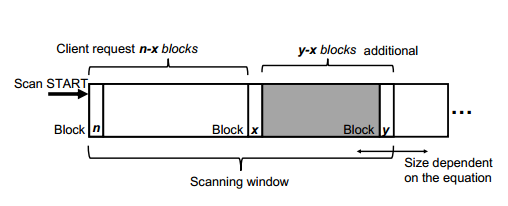
\includegraphics[width=0.7\linewidth]{image/Scanning_Window}
	\caption[پنجره پویش (\lr{Scanning Window}) ]{پنجره پویش. مطابق با تعداد بلوک‌های درخواست داده شده ($x$) و تعداد تراکنش‌های منطبق شده با درخواست مشتری در آن‌ها، احتمالا بلوک‌های بیشتری ($y$) از حافظه خوانده می‌شود تا نسبت بین بلوک‌های خوانده شده و اندازه پاسخ ثابت بماند\cite{Matetic2019}.}
	\label{fig:scanningwindow}
\end{figure}

روش دوم ارائه شده در \cite{Matetic2019} پایگاه داده ناآگاهانه نام دارد. در این روش کاربر سبک آدرس‌های مورد نظر خودش را، از طریق یک کانال محرمانه، برای SGX ارسال می‌کند و مستقیما اطلاعات مربوط به خروجی‌های خرج نشده را دریافت می‌نماید. در این روش برخلاف روش‌های پیشین و همچنین روش پنجره پویش،‌ نیاز نیست که کاربر سبک سرایند بلوک‌ها و مسیر (اثبات) درخت مرکل را دریافت و بررسی کند. در این روش کاربر به صحت عملکرد SGX و پاسخ آن اعتماد کامل دارد.
برای آنکه SGX بتواند کاربر را از صحت عملکرد خودش مطمئن سازد، 
تمام اقدامات و مقداردهی‌های اولیه به عنوان حالت اولیه ثبت می‌شود. با استفاده از آن کاربر می‌تواند مطمئن شود که کد صحیحی بر روی سامانه در حال اجرا است. به این فرایند 
%تصدیق از راه دور\RTLfootnote{\lr{Remote Attestation}}
\gls{Remote Attestation}
گفته می‌شود. تصدیق ایجاد شده، که شامل حالت اولیه است، امضا شده و برای کاربر ارسال می‌شود. کاربر می‌تواند توسط سرویس تصدیق برخطی که توسط اینتل ارائه می‌شود \cite{EPID}، امضا را بررسی نماید.

در روش پایگاه داده ناآگاهانه، SGX اطلاعات مربوط به خروجی خرج نشدهٔ تراکنش‌ها (UTXO) را در یک پایگاه داده رمزنگاری شده نگهداری می‌کند. همچنین از 
%ماشین دسترسی تصادفی ناآگاهانهٔ
%( ORAM\RTLfootnote{\lr{Oblivious Random Access Machine}})
\gls{Oblivious Random Access Machine (ORAM)}
معرفی شده در \cite{Stefanov2013} برای جلوگیری از نشت اطلاعات در هنگام دسترسی به حافظه استفاده می‌کند. به این ترتیب گره کامل متخاصم نمی‌تواند الگویی از دسترسی SGX به حافظه پیدا نماید. از طرف دیگر در این روش طول درخواست‌ها و پاسخ‌ها همواره یک مقدار ثابت است. اگر اندازه آن‌ها از آن مقدار ثابت کوتاه‌تر باشد، با لایی‌گذاری و اگر طولانی‌تر بود با تکه‌تکه کردن، به اندازه‌های ثابت تبدیل می‌شوند. در این روش SGX به تمام زنجیره بلوکی دسترسی ندارد و تنها دادهٔ UTXO را نگهداری کرده و به ازای اضافه شدن هر بلوک جدید، بعد از آن که آن بلوک را از جنبه اثبات کار و درخت مرکل درستی سنجی کرد، آن را به روزرسانی می‌کند. از آن‌جایی که UTXO در حافظه ORAM ذخیره می‌گردد، به روزرسانی آن امری نسبتا زمان‌بر، چیزی در حدود $78.5$ ثانیه، خواهد بود.

در دو روش ارائه شده در \cite{Matetic2019} بار پردازشی چندانی بر روی گره سبک قرار نخواهد گرفت. همچنین از آن‌جایی که دیگر لازم نیست برای حفظ حریم خصوصی کاربر تراکنش‌هایی مازاد به خاطر خطای نوع دو نیز دریافت شوند، پهنای باند به طور قابل ملاحظه‌ای در این دو روش نسبت به روش فیلتر بلوم کاهش پیدا می‌کند. از طرف دیگر در روش دوم (پایگاه داده ناآگاهانه) نیاز نیست که پاسخ گره کامل با اثبات‌های مرکل همراه باشد و به عبارتی گره سبک به عملکرد صحیح SGX اعتماد دارد. در نتیجه در این روش پهنای باند مصرفی بسیار کاهش پیدا می‌کند. علاوه بر مزایای ذکر شده، این روش ایراداتی نیز دارد که در ادامه به بیان آن خواهیم پرداخت.

اول از همه آنکه زمان تولید جواب در روش پنجره پویش، در صورتی که اقدامات مورد نیاز جهت جبران حمله کانال جانبی انجام شود، بسیار زمان‌بر است. به عنوان مثال برای پردازش  $100$ بلوک در این روش چیزی در حدود $73$ ثانیه زمان نیاز است. این زمان برای روش فیلتر بلوم با نرخ خطای نوع دوی $0.5$ درصد، حدود $1.1$ ثانیه است \cite{Matetic2019}. هر چند که تولید پاسخ در روش  پایگاه داده ناآگاهانه بسیار سریع‌تر انجام می‌شود، اما برای به روز رسانی داده خروجی‌ خرج نشده تراکنش‌ها نیاز به $78.5$ ثانیه زمان دارد. به عبارتی می‌توان اینطور گفت که هر ده دقیقه یک‌بار (زمان مورد نیاز برای استخراج یک بلوک جدید)، حدود یک دقیقه و هجده ثانیه،‌ صرف به روز رسانی شده و امکان پاسخ‌گویی به کاربران سبک را ندارد. مقاله \cite{Matetic2019} برای افزایش دسترس‌پذیری سیستم در شرایط به روز رسانی، پیشنهاد استفاده از دو سیستم موازی را داده است. در این شرایط نیز،‌ سیستم ارائه دهنده خدمات از وضعیت فعلی شبکه حداکثر حدود $78.5$ ثانیه عقب‌تر خواهد بود.

مشکل دیگری که روش \cite{Matetic2019} دارد، حملات فیزیکی کانال جانبی مدرنی است که SGX نسبت به آن‌ها آسیب‌پذیر است. مثلا حملات اسپکتر\LTRfootnote{\lr{Spectre}}\cite{Kocher2019}، ملت‌داون\LTRfootnote{\lr{Meltdown}}\cite{Lipp2020} و حمله \cite{Bulck2020} که به تازگی کشف شده است، می‌توانند برای استخراج کلید‌های تصدیق از ‌SGX مورد استفاده قرار گیرند. در صورتی که گره کامل متخاصم از چنین حمله‌ای بهره‌بردای کند، می‌تواند در روش پنجره پویش، حریم خصوصی کاربران سبک درخواست دهنده را نقض نماید؛ همچنین در روش پایگاه دادهٔ ناآگاهانه علاوه بر نقض حریم خصوصی کاربر سبک می‌تواند اطلاعات اشتباهی را در اختیار وی قرار دهد.

علاوه بر مشکلات ذکر شده در بالا، می‌توان به این مسئله نیز اشاره نمود که برای آنکه یک گره کامل بخواهد خدمات پیشنهاد شده در \cite{Matetic2019} را به گره‌های سبک ارائه دهد، نه تنها نیاز است که یک محیط اجرای قابل اطمینان تهیه و راه‌اندازی نماید، بلکه لازم است که منابع پردازشی قابل توجهی را برای این منظور اختصاص دهد. در نتیجه گره‌های کاملی که بتوانند چنین خدماتی ارائه دهند، محدود خواهند بود. به تبع آن کاربران سبک مجبور خواهند بود که بین گره‌های کامل محدود‌تری انتخاب کنند که این مسئله انگیزه این گره‌های کامل را برای انجام اقدامات خصمانه بیشتر خواهد کرد. از این اقدامات می‌توان به ایجاد و دنبال کردن یک انشعاب ناصحیح از زنجیره بلوکی بیت‌کوین اشاره نمود. در حالت عادی که تعداد گره‌های کامل زیاد هستند، گره سبک می‌تواند با دریافت خدمات از گره‌های کامل متعدد از صحت اطلاعات دریافتی مطمئن گردد.

از طرف دیگر، شرکت‌های محدودی مانند اینتل، تجهیزات مربوط به یک محیط اجرای قابل اطمینان را تولید و به فروش می‌رسانند. همچنین نیاز است که برای  تصدیق از راه دور عملکرد آن‌ها به سرویس‌هایی مثل \cite{EPID} وابسته بود. به بیان دیگر می‌توان این طور گفت که برای آنکه بتوان از روش \cite{Matetic2019} بهره‌برداری کرد، لازم است به شرکت‌های محدودی اعتماد شود که این خود بر خلاف ذات شبکه‌های همتابه‌همتایی مثل بیت کوین است.



\section{مقایسه}

در این فصل، ضمن آشنایی با ساز و کار فعلی شبکه‌ٔ همتا‌به‌همتای بیت‌کوین در ارسال اطلاعات مربوط به تراکنش‌های یک گره سبک با هدف حفظ حریم خصوصی وی \cite{Hearn2013}، توضیح داده شد که روش فعلی بسیار آسیب‌پذیر است و در صورتی که کاربر سبک خود اقداماتی را جهت حفظ بیشتر حریم خصوصیش انجام ندهد، عملا حریم خصوصی وی اصلا حفظ نمی‌شود.

علاوه بر این، در این فصل به بیان مفصل راه‌حل‌هایی که تا کنون برای رفع این مشکل ارائه شده‌اند، پرداخته شده است. در این قسمت این راه‌حل‌ها از سه جنبهٔ امنیت، پهنای باند مصرفی، بار پردازشی سمت گره کامل با هم مقایسه می‌شوند. که نتیجهٔ این مقایسه در جدول‌های زیر آورده شده است.

\begin{xltabular}{\textwidth}{|r|X|}
	\caption{
		مقایسهٔ امنیت روش‌های بحث شده.
		\label{table:SecurityCmp}}\\
	\hline
	\textbf{روش} & \textbf{آسیب‌پذیری‌ها} \\
	\hline 
	{%
		فیلتر بلوم \cite{Hearn2013}
	} & {%
		نرخ خطای نوع دوی عملا خیلی پایین، دسترسی به چند فیلتر بلوم از یک کاربر، کشف اولین استفاده از آدرس، تحلیل گراف تراکنش‌ها و کشف آدرس‌های مرتبط، تحلیل بسامد استفاده از آدرس، تحلیل زمان درخواست
	} \\
\hline
	{%
		اصلاح رفتار گره سبک \cite{Gervais2014}
	} & {%
		کشف اولین استفاده از آدرس، تحلیل گراف تراکنش‌ها و کشف آدرس‌های مرتبط، تحلیل بسامد استفاده از آدرس، تحلیل زمان درخواست
	}\\
\hline
	{%
		معیار حاشاپذیری-$\gamma$ \cite{Kanemura2017}
	} & {%
		دسترسی به چند فیلتر بلوم از یک کاربر، کشف اولین استفاده از آدرس، تحلیل گراف تراکنش‌ها و کشف آدرس‌های مرتبط، تحلیل بسامد استفاده از آدرس، تحلیل زمان درخواست
	}\\
\hline
	{%
		فیلتر بلوک \cite{Osuntokun2017}
	} & {%
		تحلیل گراف تراکنش‌ها و کشف آدرس‌های مرتبط، تحلیل بسامد استفاده از آدرس، تحلیل زمان درخواست
	}\\
\hline
	{%
		بازیابی اطلاعات خصوصی \cite{Qin2019}
	} & {%
		تبانی گره‌های کامل، تحلیل زیردسته‌های دستهٔ تمام-مدت مورد پرسمان واقع شده، تحلیل بسامد استفاده در زیردسته‌ها، سخت بودن راه‌اندازی یک گره کامل در نتیجه نیاز به اعتماد به گره‌های اندک موجود
	}\\
\hline
	{%
		پنجرهٔ پویش (\lr{SGX}) \cite{Matetic2019}
	} & {%
		اعتماد به سازنده‌های سخت‌افزار محیط‌های قابل اعتماد، افشای اطلاعات در صورت حملات کانال جانبی، سخت بودن راه‌اندازی یک گره کامل در نتیجه نیاز به اعتماد به گره‌های اندک موجود
	}\\
\hline
	{%
		پایگاه دادهٔ ناآگاهانه (\lr{SGX}) \cite{Matetic2019}
	} & {%
		اعتماد به سازنده‌های سخت‌افزار محیط‌های قابل اعتماد، افشای اطلاعات در صورت حملات کانال جانبی، ارسال اطلاعات نادرست در صورت حملات کانال جانبی، سخت بودن راه‌اندازی یک گره کامل در نتیجه نیاز به اعتماد به گره‌های اندک موجود
	}\\
\hline	
\end{xltabular}

\begin{xltabular}{\textwidth}{|r|X|}
	\caption{
		مقایسهٔ پهنای باند مصرفی در روش‌های بحث شده.
		\label{table:BandWidthCmp}}\\
	\hline
	\textbf{روش} & \textbf{پهنای باند} \\
	\hline 
	{%
		فیلتر بلوم \cite{Hearn2013}
	} & {%
		به خاطر به‌روز رسانی فیلتر توسط گره کامل، از خیلی کم به زیاد تغییر می‌کند. شامل تراکنش‌ها و اثبات مرکل
	} \\
	\hline
	{%
		اصلاح رفتار گره سبک \cite{Gervais2014}
	} & {%
		متوسط - نرخ خطای نوع دو بالاتر از روش \cite{Hearn2013}. شامل تراکنش‌ها و اثبات مرکل.
	}\\
	\hline
	{%
		معیار حاشاپذیری-$\gamma$ \cite{Kanemura2017}
	} & {%
		کم
	}\\
	\hline
	{%
		فیلتر بلوک \cite{Osuntokun2017}
	} & {%
		برای گره‌های مختلف با تعداد تراکنش‌های مختلف متفاوت است.
	}\\
	\hline
	{%
		بازیابی اطلاعات خصوصی \cite{Qin2019}
	} & {%
		خیلی زیاد. اندازهٔ فایل مانیفست تمام-مدت $3.30$ گیگابایت
	}\\
	\hline
	{%
		پنجرهٔ پویش (\lr{SGX}) \cite{Matetic2019}
	} & {%
		خیلی کم. شامل تراکنش‌های مرتبط و اثبات مرکل. بدون خطای نوع دو.
	}\\
	\hline
	{%
		پایگاه دادهٔ ناآگاهانه (\lr{SGX}) \cite{Matetic2019}
	} & {%
		ناچیز. شامل تراکنش‌های مرتبط بدون نیاز به اثبات مرکل و بدون خطای نوع دو.
	}\\
	\hline	
\end{xltabular}

\begin{xltabular}{\textwidth}{|r|X|}
	\caption{
		مقایسهٔ پردازش سمت گره کامل در روش‌های بحث شده.
		\label{table:ProcCmp}}\\
	\hline
	\textbf{روش} & \textbf{پردازش سمت گره کامل} \\
	\hline 
	{%
		فیلتر بلوم \cite{Hearn2013}
	} & {%
		زیاد - برای هر فیلتر بلوم باید چکیدهٔ تمام داده‌های تراکنش‌های یک بلوک $k$ بار حساب شود. 
	} \\
	\hline
	{%
		اصلاح رفتار گره سبک \cite{Gervais2014}
	} & {%
		زیاد - برای هر فیلتر بلوم باید چکیدهٔ تمام داده‌های تراکنش‌های یک بلوک $k$ بار حساب شود.
	}\\
	\hline
	{%
		معیار حاشاپذیری-$\gamma$ \cite{Kanemura2017}
	} & {%
		زیاد - برای هر فیلتر بلوم باید چیکدهٔ تمام داده‌های تراکنش‌های یک بلوک $k$ بار حساب شود.
	}\\
	\hline
	{%
		فیلتر بلوک \cite{Osuntokun2017}
	} & {%
		کم - فقط یک بار باید چکیدهٔ تمام داده‌های تراکنش‌های یک بلوک حساب شده و برای فشرده‌سازی، کدگذاری شوند.
	}\\
	\hline
	{%
		بازیابی اطلاعات خصوصی \cite{Qin2019}
	} & {%
		زیاد. به ازای استخراج یک بلوک جدید باید دستهٔ هفتگی به روز رسانی شود.
	}\\
	\hline
	{%
		پنجرهٔ پویش (\lr{SGX}) \cite{Matetic2019}
	} & {%
		خیلی خیلی زیاد. به ازای درخواست هر کاربر سبک باید تمام اثبات‌های مرکل تمام تراکنش‌های چند بلوک را حساب کند. تعداد بلوک‌های محاسبه شده با توجه به درخواست کاربر تعیین می‌شود.
	}\\
	\hline
	{%
		پایگاه دادهٔ ناآگاهانه (\lr{SGX}) \cite{Matetic2019}
	} & {%
		زیاد. به ازای استخراج هر بلوک جدید، باید پایگاه‌داده ناآگاهانه را به روزرسانی کند.
	}\\
	\hline	
\end{xltabular}

		% فصول سوم: مروری بر کار‌های انجام شده
% !TeX root=../main.tex
\chapter{ارائهٔ روش}
\label{proposed}
%\thispagestyle{empty} 
\section{مقدمه} 
روش k-گمنامی اولین بار در مقاله \cite{Sweeney2002} معرفی شده است. با این روش می‌توان اطلاعات مرتبط با افرادی  را که می‌خواهیم گم‌نامی آن‌ها حفظ شود، منتشر نمود. از این روش در سرویس‌های مبتنی بر مکان نیز استفاده می‌شود \cite{Niu2015} . در این سرویس‌ها عموما لازم است کاربر برای دریافت خدمات مرتبط با موقعیت جغرافیایی فعلی خود، اطلاعات مکانی خود را در اختیار ارائه دهنده این خدمات قرار دهد. در  \cite{Niu2015} شرح داده شده است که در صورتی که کاربر اطلاعات مکانی خود را با اطلاعاتی مصنوعی که نشان‌دهنده مکان‌های دیگری هستند ترکیب کند و مجموعه آن‌ها را به سرویس‌دهنده ارسال نماید، می‌تواند تا حدی اطلاعات مکانی خود را پنهان کند. مقاله \cite{Niu2015} با استفاده از معیار آنتروپی توضیح داده که در صورتی که کاربر اطلاعات مصنوعی را به نحوی انتخاب نماید که نرخ (احتمال) پرسمان اطلاعات مربوط به آن مکان‌ها با نرخ پرسمان اطلاعات مکانی خود یکسان باشد، آنتروپی تشخیص مکان کاربر توسط سرویس‌دهنده بیشتر می‌شود. به بیان دیگر سرویس‌دهنده در مورد آن که کدام یکی از موقعیت‌های درخواست داده شده حقیقی و مربوط به کاربر هستند با ابهام بیشتری مواجه خواهد شد.

در این مقاله سعی داریم برخلاف روش مبتنی بر فیلتر بلوم که آدرس‌های مصنوعی به صورت کورکورانه و تصادفی اتخاذ می‌شدند آدرس‌های مصنوعی به نحوی اتخاذ شوند که دارای نرخ پرسمان تقریبا یکسانی با آدرس کاربر درخواست دهنده باشند. در ابتدا تعاریف ریاضی مسئله را بیان کرده و سپس مروری می‌کنیم بر ویژگی‌هایی که لازم است پروتکل ارائه شده از آن‌ها برخوردار باشد.



\subsection{تعریفات ریاضی}




در این مقاله کاربر سبک $i$ام را با $l_i$ نمایش می‌دهیم. مجموعه تمام گره‌های سبک در شبکه به صورت $LW = \{l_1,..., l_M\}$ است که $M$ تعداد کل این گره‌ها است. گره‌ کامل $j$ام به صورت $f_j$ و مجموعه تمام گره‌های کامل به صورت $FN=\{f_1,..., f_W\}$ و تعداد کل گره‌های کامل با $W$ نمایش داده می‌شود. تعداد کل آدرس‌های بیت‌کوین $N$ است و $A=\{a_1,..., a_N\}$ مجموعه تمام آدرس‌ها است. هر آدرس شبکه متعلق به یک گره کامل یا یک گره سبک است. همچنین هر گره می‌تواند مالک چند آدرس باشد. آدرس‌های مربوط به گره سبک $l_i$، که مالک
$C_{l_i}$ 
عدد آدرس است، مجموعه 
$A_{l_i}=\{a_{l_{i1}},... , a_{l_{iC_{l_i}}}\}$
را تشکیل می‌دهد. به همین ترتیب آدرس‌های مربوط به هر کدام از گره‌های کامل تعریف می‌شوند.
%به طوری که:
%\begin{equation}
%	\forall 1<i<M, 1<j<W : A_i, A_j \subset A
%\end{equation}

کاربران سبک اطلاعات جدید مربوط به آدرس‌هایشان را از گره‌های کامل پرسمان می‌کنند. متغیر تصادفی $X_{{a_n}j}$ به این ترتیب تعریف می‌شود که گره کامل $f_j$ آخرین درخواستی که دریافت می‌کند مربوط به آدرس $a_n$ باشد. با توجه به قانون اعداد بزرگ در احتمال، امید ریاضی $X_{{a_n}j}$‌ برابر با تعداد  دفعات درخواست‌های مربوط به آدرس $a_n$ به تعداد کل درخواست‌هایی است که 
$f_j$
، به طوری که
$(1<j<W)$
، دریافت کرده است.
\begin{equation}
E\{X_{{a_n}j}\} = \frac{Q_{{a_n}j}}{Q_{Tj}} \label{eq:1}
\end{equation}
در معامله \eqref{eq:1}،
$E\{X_{{a_n}j}\}$
امید ریاضی پرسمان آدرس $a_n$ از گره کامل
$f_j$ 
است و
$Q_{{a_n}j}$
و
$Q_{Tj}$
به ترتیب تعداد دفعات پرسمان آدرس $a_n$ و تعداد دفعات کل پرسمان‌ها از گره کامل $f_j$ هستند. همچنین می‌توان با استفاده از قانون اعداد بزرگ بورل، احتمال رخداد پیشامد پرسمان $a_n$ در آخرین درخواست انجام شده از گره کامل $f_j$ را برابر امید ریاضی
$E\{X_{{a_n}j}\}$
قرار داد. با توجه به اینکه کاربران سبک در هر نوبت پرسمان به صورت تصادفی یک گره کامل را انتخاب می‌کنند، می‌توان فرض کرد که احتمال پرسمان آدرس‌ها در تمام گره‌های کامل با هم برابر است.
\begin{equation}
Pr\{a_{n}\} = Pr\{a_{nj}\} = E\{X_{{a_n}j}\}, 0<j<M \label{eq:2}
\end{equation}
در معادله \eqref{eq:2}، 
$Pr\{a_{nj}\}$
احتمال پرسمان آدرس $a_n$ از گره کامل
$f_j$ 
است. لازم به ذکر است که احتمال درخواست آدرس‌های مربوط به هر گره‌ کاملی برابر صفر است. چرا که این گره‌ها خودشان وضعیت کامل زنجیره بلوکی را ذخیره کرده‌اند و از گره کامل دیگری در مورد اطلاعات مربوط به آدرس‌هایشان پرسمان انجام نمی‌دهند.
\begin{equation}
Pr\{{a_n}\} = 
\begin{cases}
0, & \text{if}\ a_n \in A_{f_j},\ \ \forall_{j} : 1<j<W \\
Pr\{{a_{l_{ic}}}\}, & \text{if}\ a_n = a_{l_{ic}} \in A_{l_i},\ \ \forall_{i,c} : 1<i<M,\  1<c<C_{l_i}
\end{cases} \label{eq:3}
\end{equation} 

\subsection{ملزومات پروتکل}
\label{subsubsection:4.2}
پیش از پرداختن به ساختار طراحی پروتکل لازم است ویژگی‌هایی که پروتکل باید از آن‌ها برخوردار باشد بررسی شوند. با توجه به هدف پروتکل، که حفظ حریم خصوصی کاربران دارای گره‌های سبک است، لازم است که به مصون ماندن پروتکل نسبت به حملاتی که حریم خصوصی افراد را نقض می‌کنند، توجه ویژه داشت. از طرف دیگر از آن‌جا که کاربران دارای گره‌های سبک امکان پردازش‌ و ذخیره‌سازی حجم بالای اطلاعات را ندارند، همچنین پهنای باند آن‌ها محدود و پر هزینه است، لازم است پروتکل طراحی شده، کمترین میزان بار محاسباتی،‌ مصرف حافظه و پهنای باند را در سمت کاربران سبک داشته باشد. لازم به ذکر است، در صورت وجود فرایند‌های پیچیده در پروتکل، آسیب‌پذیری‌ها و حفره‌های امنیتی زیادی در پروتکل و پیاده‌سازی‌های آن وجود خواهد داشت. از این رو در این پروتکل سعی شده است که تا جای ممکن از فرایند‌های ساده‌ای که پیش از این در کاربرد‌های مختلف آزموده شده‌اند استفاده گردد.

علاوه بر این نباید تغییرات عمده‌ای در ساز و کار گره‌های کامل اعمال کرد و آن‌ها را ملزم به استفاده از ابزارهایی سخت‌افزاری، غیر از سخت افزار مورد نیاز یک گره کامل در شرایط فعلی، نمود. همچنین نباید از نرم‌افزارهایی با مالکیت اختصاصی و متن بسته استفاده شود. این دو کار نه تنها به خاطر دشوار کردن و هزینه‌بر کردن راه‌اندازی یک گره‌کامل، تعداد آن‌ها را در شبکه کمتر می‌کند و منجر به متمرکز شدن شبکه می‌شود، بلکه پروتکل بیت‌کوین را که یک پروتکل بی‌نیاز به اعتماد به یک طرف سوم است، ملزم به اعتماد به شرکت‌های تولید سخت‌افزار‌ و نرم‌افزار‌ به خصوصی می‌کند که وجود درهای پشتی در محصولات آن‌ها اجتناب ناپذیر خواهد بود. 

در ادامهٔ این بخش محدودیت‌ها و  ضوابطی را برای این پروتکل بیان می‌کنیم تا حریم خصوصی کاربر حفظ شده و  همچنین بار محاسباتی، مصرف حافظه و پهنای باند چندانی به طرفین پروتکل اضافه نشود.

نخست، برای آنکه گره کامل $f_j \in FN$ نتواند آدرس $a_{l_{ic}} \in A_{l_i}$ مربوط به گره سبک درخواست دهنده $l_i$ را تشخیص دهد، گره سبک $l_i$ باید اطلاعات مربوط به آدرس خود را به همراه اطلاعت مربوط به $k-1$ عدد از آدرس‌های مصنوعی را همزمان درخواست دهد، به طوری که
$ a_n \in A \textbackslash \{a_{l_{ic}}\}$
. اگر آدرس‌های مصنوعی به نحوی انتخاب شوند که نرخ پرسمان آن‌ها، در زمان درخواست، کمتر از آدرس اصلی باشند، یا اصلا وجود نداشته باشند
($a_n \notin A$)،
گره کامل می‌تواند با احتمال بالاتری آدرس درخواست دهنده را در میان آدرس‌های مصنوعی درخواست داده شده حدس بزند. از این رو باید کاربر سبک آدرس‌های مصنوعی را به نحوی اتخاذ نماید که احتمال درخواست تقریبا برابری با آدرس حقیقی خود داشته باشند، تا گم‌نامی کاربر سبک درخواست دهنده بیشتر حفظ ‌شود. 

دوم، واضح است که محاسبه و پیدا کردن حداقل $k-1$ آدرسی که دارای احتمالی برابر با آدرس کاربر درخواست دهنده باشند، بدون دسترسی به اطلاعات تراکنش‌ها و تناوب درخواست‌ آن‌ها از گره‌های کامل، امری غیر ممکن است. از طرف دیگر اگر کاربر سبک بخواهد این اطلاعات را به طور مستقیم از گره کامل، که دارای تمام این اطلاعات است، دریافت نماید، مشکلاتی اساسی پدید خواهد آمد. در سناریوی پیش رو به دو مورد از آن‌ها اشاره خواهیم نمود.

فرض کنید، $l_i$ در مرحله اول احتمال درخواست آدرس $c$ام خود، یعنی $a_{l_{ic}}$، را حساب نماید. بعدا توضیح داده خواهد شد که این محاسبه بدون نیاز به افشای آدرس به شخص سومی و صرفا بر اساس سوابق کیف پول کاربر قابل انجام است. سپس، احتمال به دست آمده را (بدون ذکر
$a_{l_{ic}}$
) به گره کامل 
$f_{j_1}$
ارسال کرده و  درخواست $k-1$ آدرس با احتمال پرسمان برابر
$Pr\{{a_{l_{ic}}}\}$
بدهد. در مرحله دوم، کاربر آدرس خودش را در میان آدرس‌های مصنوعی هم احتمال قرار داده و اطلاعات مربوط به مجموعه $k$ آدرس حاصل را از یک گره کامل دیگر $f_{j_2}$ یا همان گره کامل پیشین درخواست نماید.  در این سناریو اگر کاربر اطلاعات مجموعه آدرس‌ها را از همان $f_{j_1}$ درخواست نماید، $f_{j_1}$ با توجه به سوابق آدرس‌هایی که قبل‌تر ارسال کرده بوده، متوجه آدرس کاربر، که آدرس جدیدیست و در سوابق اخیرش موجود نیست، می‌شود و آدرس کاربر نزد گره کامل فاش می‌گردد. 

کاربر برای حفظ گم‌نامیش می‌تواند از گره‌ دیگری، مثل $f_{j_2}$ اطلاعات مربوط به مجموعه آدرس‌های هم احتمال را درخواست نماید. در این حالت نیز، در صورتی که $f_{j_1}$ با $f_{j_2}$ تبانی نموده و سوابقشان را با هم به اشتراک بگذارند، طبق روندی که پیش‌تر گفته شد، آدرس فرد درخواست دهنده قابل تشخیص خواهد بود. برای رفع این مشکل کاربر می‌تواند در مرحله اول آدرس‌های هم احتمال را از چند گره متفاوت دریافت نماید و در مرحله دوم زیرمجموعه‌ای تصادفی از تمام آن‌ها را انتخاب و حاصل را به چند بخش تقسیم کرده و هر قسمت را از گره‌ای مجزا درخواست نماید. در این حالت احتمال تشخیص آدرس توسط گره‌هایی که تبانی کرده‌اند کاهش می‌یابد. با این حال، در این روش کاربر سبک باید در صحت هم احتمال بودن آدرس‌های دریافتی به گره‌(ها)ی کامل اعتماد نماید چرا که تصدیق و صحت‌سنجی آن‌ها بدون دسترسی به اصل داده‌ها امکان‌پذیر نیست. به عنوان مثال، در مرحله اول یک گره کامل می‌تواند با ارسال آدرس‌هایی که نرخ پرسمان یکسان، اما متفاوت با نرخ پرسمان آدرس درخواست داده‌شده، داشته باشند، منجر به افشای آدرس کاربر گردد.

از این حیث، لازم است که پروتکل طراحی شده به کاربر سبک اجازه دهد بدون نیاز به فاش کردن اطلاعاتش و همچنین اعتماد به اطلاعات ارسال شده از یک طرف سوم، آدرس‌هایی هم احتمال با آدرس خودش را اتخاذ نموده و مجموعه آن‌ها را از گره کامل پرسمان نماید.

سوم، باید این امر مهم را در نظر بگیریم که کاربران سبک بسیار زیادی هستند که برای به روز رسانی اطلاعاتشان، از طریقی غیر از شبکه‌های حافظ گم‌نامی (مانند تور\RTLfootnote{\lr{Tor}}\cite{torproject}، کراودز\RTLfootnote{\lr{Crowds}}\cite{reiter1998crowds} و غیره)، با گره‌های کامل تبادل اطلاعات انجام می‌دهند. در این صورت مبداء ارسال پرسمان‌های یک کاربر سبک با تقریب خوبی یکسان خواهد ماند. گره کامل متخاصم می‌تواند سابقه‌ای را از پرسمان‌های یک کاربر سبک $l_i$ تشکیل دهد. در این صورت اگر $l_i$ آدرس‌های خودش را، یعنی
$a_{l_{ic}}$
به طوری که
$1<c<C_{l_i}$،
مدام در مجموعه‌ای متفاوت از آدرس‌های هم احتمال قرار دهد، گره متخاصم می‌تواند با اشتراک گیری بین سوابق پرسمان کاربر سبک، به مجموعه‌ای محدودتر از آدرس‌هایی دست پیدا کند که در تمام یا اکثر پرسمانهای آن کاربر وجود داشته‌اند. در نتیجه با احتمال بیشتری می‌تواند آدرس کاربر را تشخیص دهد. برای حفظ گم‌نامی کاربر سبک در برابر این حمله، کاربر سبک باید از مجموعه هم احتمال و تا حد امکان ثابتی استفاده نماید.

در این بخش ملزوماتی برای پروتکل طراحی شده مطرح شدند که علاوه بر آنکه این پروتکل اثر نامطلوبی بر توزیع‌شدگی و امنیت بیت‌کوین نداشته باشد، در برابر حملاتی که ممکن است منجر به فاش شدن آدرس‌های مربوط به یک کاربر سبک گردد مقاوم باشد.

\subsection{ساختار پروتکل}
در این قسمت به توصیف پروتکل پرداخته می‌شود. پروتکل ارائه شده به دو بخش تقسیم می‌گردد. بخش اول شامل فرایندی است که در گره‌های کامل انجام می‌گردد. در این بخش، احتمال پرس‌وجوی تمام آدرس‌های بیت‌کوین ($A$) محاسبه شده و به آدرس‌هایی با احتمال نزدیک به هم تقسیم می‌شوند. به هرکدام از این قسمت‌ها، تکه‌ (Chunk) گفته می‌شود. بخش دوم شامل فرایندی است که گره سبک به صورت آفلاین و بدون نیاز به طرف سومی انجام می‌دهد تا بفهمد که آدرس مربوط به آن در کدام تکه قرار دارد.

در طراحی این پروتکل فرض می‌کنیم که احتمال پرسمان اطلاعات مربوط به هر آدرس $a_n$، به شرطی که مربوط به یک گره کامل نباشد، متناسب است با احتمال استفاده از آن آدرس در شبکه بیت‌کوین. یعنی فرض شده است که هرچه یک کاربر سبک از یک آدرس بیشتر استفاده نماید،‌ بیشتر تمایل دارد اطلاعاتش را در مورد آن آدرس از طریق پرسمان از گره‌های کامل به روزرسانی نماید. به بیان دیگر می‌توانیم بنویسیم:
\begin{equation}
Pr\{{a_n}\} \propto p(a_n) \triangleq \frac{NT_{a_n}}{\sum_{m=1}^{N}NT_{a_m}}; \forall i \  a_n \in A_{l_i}  \label{eq:4}
\end{equation}

در معادله \eqref{eq:4}، 
$NT_{a_n}$
تعداد تراکنش‌هایی هستند که در آن‌ها از آدرس $a_n$ به عنوان ورودی یا خروجی استفاده گردیده و در زنجیره بلوکی بیت‌کوین ثبت شده است. $p(a_n)$ احتمال استفاده از آدرس $a_n$ در شبکه بیت‌کوین تعریف می‌شود. با استفاده از تعریف  \eqref{eq:4} می‌توانیم به تعریفی قابل اجماع از احتمال پرسمان یک آدرس دست پیدا کنیم. دستیابی به این تعریف با توجه به توزیع شدگی و شفافیت و همچنین یکتا بودن وضعیت زنجیره بلوکی در میان تمام گره‌های شبکه قابل انجام است.  

\subsubsection{محاسبه مستقل از دیگر آدرس‌ها}
\label{subsubsection:4.3.1}
کاربران سبک  باید بتوانند بدون نیاز به هر درخواست اطلاعات اضافه‌ای از گره کامل، محاسبه نمایند که آدرس‌های آن‌ها در کدام تکه قرار گرفته است. فرایند انجام این محاسبه به طور کامل در بخش \ref{subsubsection:4.3.3} توضیح داده شده است. در این بخش می‌خواهیم پروتکل را به نحوی طراحی کنیم که گره‌های سبک بدون نیاز به پرسیدن چیزی از گره دیگری، بتوانند تکه مربوط به خود را مشخص نماید. در گام اول لازم است به این موضوع اشاره شود که گره‌های سبک امکان محاسبه $NT_{a_n}$ مربوط به آدرس خود را به صورت آفلاین و با توجه به سوابق تراکنش‌هایشان دارند. به خاطر یکسان بودن
$\sum_{m=1}^{N}NT_{a_m}$
نیازی نیست که کاربران سبک از آن اطلاع داشته باشند.

مسئله دیگری که لازم است مورد توجه قرار گیرد، ارائه روشی برای محاسبه آدرس‌های هر تکه به صورتی است که نه تنها با تغییر عمده نرخ پرسمان یک آدرس، آدرس در تکه‌ای جدا و متناسب با نرخ جدید قرار بگیرد و در تکه قبلی نماند، بلکه با توجه به آنچه در بخش \ref{subsubsection:4.2} بحث شده بود، لازم است که تکه‌ها نسبت که تغییرات اندک نرخ پرسمان آدرس‌ها مقاوم باشند. تغییر خیلی کند تکه‌ها باعث می‌شود که آنتروپی هر تکه کاسته شود و از طرف دیگر تغییر سریع تکه‌ها باعث می‌شود که گره کامل با اشتراک گیری درخواست‌هایی که از یک منبع ثابت ارسال می‌شوند، به تعداد محدودتری از آدرس‌های محتمل برای گره سبک درخواست دهنده دست یابد.

برای رسیدن به این هدف ابتدا تعریفی از امتیاز هر آدرس در زمان $t_0$ به صورت 
$s_{a_n}^{t_0}$
تعریف می‌کنیم. مجموعه تمام این امتیاز‌ها در یک زمان خاص، حالت سیستم در آن زمان نامیده می‌گردد. 
\begin{equation}
\forall\ a_n\ \text{in}\  A\  \text{at}\  t_0: S^{t_0} = [s_{a_1}^{t_0}, ..., s_{a_n}^{t_0}]^T  
\label{eq:5}
\end{equation}
که
$S^{t_0}$
حالت سیستم در پنجره زمانی $t_0$ است. پنجره زمانی با $W$ مشخص شده و به این صورت تعریف می‌شود: پارامتر $W$ برابر با تعداد بلوک‌هایی است که نشان‌دهنده یک واحد زمانی هستند. بعد از استخراج $W$ بلوک و ثبت آن در زنجیره بلوکی بیت‌کوین، حالت سیستم با توجه به $W$ بلوک اخیر استخراج شده به روزرسانی می‌گردد. به این ترتیب امتیاز آدرس $a_n$ در پنجره زمانی  $t_0$  ($W^{t_0}$)به صورت $s_{a_n}^{t_0}$ نمایش داده شده و به صورت معادله \eqref{eq:6} تعریف می‌شود.
\begin{equation}
s_{a_n}^{t_0} = \beta NT_{a_n}^{t_0} + (1-\beta) s_{a_n}^{t_{-1}}
\label{eq:6}
\end{equation}

که
$0<\beta<1$
و
$NT_{a_n}^{t_0}$
تعداد تراکنش‌هایی است که شامل آدرس $a_n$ در ورودی یا خروجیشان بوده‌اند و در بلوک‌های موجود در پنجره زمانی $W^{t_0}$ ظاهر شده‌اند است. به این ترتیب حالت کلی سیستم ($S^{t_0}$ ) به صورت معادله \eqref{eq:7} به روزرسانی می‌شود.
\begin{equation}
S^{t_0} = \beta NT_{A}^{t_0} + (1-\beta) S^{t_{-1}}
\label{eq:7}
\end{equation}
که 
$NT_{A}^{t_0} = [NT_{a_1}^{t_0}, ..., NT_{a_N}^{t_0}]^T$
است. به این ترتیب توانستیم امتیاز هر کدام از آدرس‌ها را مستقل از آدرس‌های دیگر محاسبه نموده و با تنظیم پارامتر $\beta$ و اندازه $W$ سرعت تغییرات تکه‌ها را تنظیم نماییم. اندازه پنجره‌های زمانی نیز بر اساس تعداد بلوک‌های استخراج شده تعیین می‌شوند. به خاطر آنکه زمان بین استخراج دو بلوک تقریبا زمان ثابتی و برابر با ۱۰ دقیقه فرض می‌شود، زمان به روزرسانی امتیاز هر کدام از آدرس‌ها تقریبا ثابت خواهد بود. به عنوان مثال اگر اندازه پنجره زمانی ۱۴۴ بلوک در نظر گرفته شود، تقریبا هر ۲۴ ساعت یک بار امتیاز آدرس‌ها به روز رسانی می‌گردد.  


\subsubsection{تعیین و انتشار تکه‌ها}
\label{subsubsection:4.3.2}
در قسمت قبل، برای هر آدرس امتیازی در نظر گرفته شد و توضیح داده شد که چطور در هر پنجره زمانی وضعیت امتیاز تمام آدرس‌ها به روز رسانی می‌گردد. در این بخش با توجه به چگونگی توزیع امتیاز آدرس‌ها، که در شکل \ref{fig:log2scale} قابل مشاهده است، مرز بین تکه‌ها و تعداد اعضا هر تکه را به نحوی انتخاب می‌کنیم که نه تنها باعث کاهش امنیت و گم‌نامی گره‌های سبک نگردد، بلکه پهنای باند مصرف شده جهت پرسمان تمام آدرس‌های یک تکه مقرون به صرفه باشد.

با توجه به معادله \eqref{eq:3} احتمال پرسمان آدرس $a_n$ به شرطی که برای یک گره کامل نباشد برابر $Pr\{{a_n}\}$ و مخالف صفر است. اگر گره سبک $l_i$ بخواهد اطلاعات مربوط به آدرس $a_{l_{ic}}$ را که مربوط به خودش است درخواست نماید لازم است اطلاعات مربوط به آدرس‌های هم احتمال با خودش را که یک تکه‌ را تشکیل می‌دهند (مثلا تکه شماره $\gamma$) دریافت نماید. تعداد اعضای این تکه را با $K_\gamma$ نمایش می‌دهیم. از منظر گره کامل هر کدام از $K_\gamma$  آدرس‌ موجود در تکه درخواست داده شده ممکن است برای درخواست دهنده ($a_{l_{ic}}$ ) باشد. احتمال آنکه هر کدام از آدرس‌های تکه، آدرس مورد نظر باشد را با $q_k$ نشان می‌دهیم که $k=(1, 2, ..., K_\gamma)$. به این ترتیب $q_k$ به صورت زیر تعریف می‌شود.

\begin{equation}
q_k = \frac{Pr\{a_{\gamma k}\}}{\sum_{m=1}^{K_\gamma}Pr\{a_{\gamma m}\}}; \quad \sum_{k=1}^{K_\gamma} q_k = 1
\label{eq:8}
\end{equation}

که $Pr\{a_{\gamma m}\}$ احتمال پرسمان آدرس $k$ام مربوط به تکه‌ $\gamma$ است. به این ترتیب آنتروپی تشخیص آدرس مورد نظر از میان آدرس‌های تکه $\gamma$ به صورت معادله \eqref{eq:9} قابل محاسبه خواهد بود:
\begin{equation}
H = -\sum_{k=1}^{K_\gamma} q_k . \log_2 q_k
\label{eq:9}
\end{equation}

که هر چه آنتروپی ($H$) بزرگ‌تر باشد به معنی حفظ بیشتر گم‌نامی آدرس مورد نظر است است. زمانی این مقدار ماکزیمم است که تمام $K_\gamma$ عضو تکه، احتمالی برابر داشته باشند. این مقدار ماکزیمم برابر $H_{max} = \log_2K_\gamma$ است.

با فرض اینکه احتمال پرسمان یک آدرس مربوط به گره سبک متناسب است با احتمال قرارگیری این آدرس در تراکنش‌های موجود در زنجیره بلوکی بیت‌کوین (معادله \eqref{eq:4}) می‌توانیم برای تعیین  تکه‌ها و ساخت آن‌ها با توجه به امتیاز آدرس‌ها (فرمول \eqref{eq:5}) عمل نماییم. جهت نحوه مرزبندی تکه‌ها لازم است به نکات زیر توجه شود:

\begin{enumerate}
	\item{%
		هرچه مقدار $K_\gamma$ برای تکه $\gamma$ بیش‌تر باشد، آنتروپی آن بیشتر خواهد بود. بالا رفتن $K_\gamma$ باعث می‌شود که کاربر سبک به ازای هر درخواست، اطلاعات اضافه بیشتری را دریافت نماید. در نتیجه پهنای باند و ترافیک زیادی مصرف نماید. 	
	}
	\item{%
		با توجه به شکل \ref{fig:log2scale} مشاهده می‌شود که اکثر آدرس‌های استفاده شده در بیت‌کوین دارای امتیازی کمتر از یک هستند و آدرس‌هایی که امتیاز آن‌ها بیشتر از یک است بسیار کم و پراکنده هستند. از این رو اگر مرز بین تکه‌‌ها به صورت توان‌های دو
		$(..., 2^{-2}, 2^{-1}, 2^{0}, 2^{1}, 2^{2},...)$
		انتخاب شوند، در آدرس‌هایی با امتیاز کمتر از ۱، مقدار آدرس‌های تقریبا یکسانی در هر تکه قرار خواهند گرفت.
	}
	\item{%
		این شیوه قسمت‌بندی، امنیت و گم‌نامی زیادی برای آدرس‌های پر استفاده ایجاد نمی‌کند. زیرا اولا، تعداد اعضای تکه‌های آدرس‌های پر استفاده کمتر است. ثانیا، مرز این تکه‌ها گستره‌تر بوده که باعث می‌شود که آدرس‌هایی با رنج وسیعی از احتمال پرسمان را در خود جایی دهد. با این حال می‌توان استدلال کرد که آدرس‌های پر استفاده، به منظور حفظ بیشتر امنیت، مربوط به گره‌های کامل هستند یا اینکه بهتر است دارندگان این آدرس‌ها به جای استفاده از یک گره سبک،  یک گره کامل راه‌اندازی نمایند. 
	}
	\item{%
		با توجه به اینکه تکه‌های مربوط به آدرس‌های کم استفاده (با امتیاز کمتر از ۱) تعداد اعضای زیادی خواهند داشت و بارگیری آن‌ها توسط گره سبک مصرف زیاد پهنای باند و ترافیک شبکه را به همراه خواهد داشت، می‌توان از دو رویه برای آن‌ها استفاده نمود. یک، از توان‌های اعشاری برای جداسازی تکه‌های آدرس‌های کم‌ استفاده بهره برد. دو، آدرس‌های مربوط به یک تکه با اعضای زیاد را به ترتیب الفبا مرتب نمود و با توجه به حروف الفبا آن‌ها را تقسیم بندی نمود. به عنوان مثال آدرس‌هایی مربوط به یک تکه که با
		\lr{bc1qaaa}
		آغاز می‌شوند درون یک زیر تکه قرار بگیرند و آدرس‌هایی که با \lr{bc1qaac} شروع می‌شوند در یک زیر تکه دیگر قرار گیرند (در استاندارد آدرس بک-۳۲ \RTLfootnote{\lr{Bech-32}} از کاراکتر b استفاده نمی‌شود \cite{Wuille2017}). روش دوم از روش اول برتری دارد. از آن جهت که در روش اول تغییرات تکه‌ها افزوده خواهد شد. در بخش \ref{subsubsection:4.2} توضیح داده شد که تغییرات زیاد تکه‌ها باعث کاهش گم‌نامی خواهد شد.
	}
	
\end{enumerate}
در این بخش به شیوه بهینه تشکیل تکه‌ها و اهمیتی که بر حفظ گم‌نامی کاربران سبک ایفا می‌کند پرداخته شد. تکه‌های تشکیل شده در این روش در تمام شبکه، که یک زنجیره بلوکی واحد را به اشتراک می‌گذارند، یکتا است. به این ترتیب هر آدرس  در زمان $t_0$ تنها در یک تکه به خصوص قرار خواهد داشت. تشخیص این که گره کاربر سبک در کدام تکه قرار دارد، به صورت آفلاین و بدون نیاز به درخواست اطلاعات اضافه‌ای، توسط خود کاربر قابل انجام است. از این رو،‌ کاربر می‌تواند تنها با ارسال شماره تکه ($\gamma$) و زیرتکه (جداسازی الفبایی) به صورت امن به اطلاعات مربوط به آدرس خودش دست پیدا کند.


\begin{figure}[t]
	\centering
	\includegraphics[width=0.7\linewidth]{/home/taghi/Projects/Bitcoin_Address_Extractor/Analysis/Log2_scale}
	\caption[امتیاز آدرس‌های بیت‌کوین در مقیاس لگاریتمی]{امتیاز آدرس‌های بیت‌کوین در مقیاس لگاریتمی از تاریخ ۲۶ ژوئن ۲۰۱۹ الی ۰۲ دسامبر ۲۰۱۹}
	\label{fig:log2scale}
\end{figure}


\subsubsection{محاسبه آفلاین در سمت کاربر سبک}
\label{subsubsection:4.3.3}
تا اینجا، نحوه تکه‌بندی آدرس‌ها با توجه به امتیاز هر آدرس، که مطابق معادله \eqref{eq:6} محاسبه گردید، توضیح داده شد. طراحی پروتکل به نحوی انجام شد که کاربران سبک بتوانند بدون نیاز به ارسال هیچ اطلاعات اضافه‌ای، از تکه‌ای که مربوط به خودشان است آگاه شوند. از این رو محاسبه آفلاین تکه در سمت کاربر به امری ساده تبدیل شد. در این بخش به نحوه انجام این محاسبه خواهیم پرداخت.

کاربر سبک همگام با شبکه، سرایند تمام بلوک‌های زنجیره بلوکی را دارد و همچنین می‌داند که تمام تراکنش‌هایی که در آن‌ها از آدرس وی استفاده شده است، در کدام بلوک‌ها قرار دارند. از این رو کاربر سبک می‌تواند به راحتی با توجه به سوابقی که در اختیار دارد و با استفاده از فرمول \eqref{eq:6} از شماره تکه‌ای که شامل آدرس خودش است مطلع شود. کاربر سبک همچنین می‌تواند به راحتی تشخیص دهد که آدرسش، با توجه به تقسیم‌بندی الفبایی، در کدام زیر تکه قرار دارد. 

اگر کاربر سبک تمام سوابق خودش را از دست دهد، می‌تواند زیر تکه متناسب با آدرسش را از تمام تکه‌های موجود درخواست دهد. استفاده از روش چینش الفبایی کمک می‌کند که کاربر سبک  زیرتکه‌های کمتری را امتحان کرده و درنتیحه ترافیک شبکه کمتری مصرف نماید.

از آن‌جایی که محاسبهٔ امتیاز هر آدرس با توجه به زنجیره بلوکی تعیین می‌شود، مقدار آن قابل اجماع است. از این رو گره‌های کامل می‌توانند به صورت روزانه (به ازای هر $144$ بلوک) امتیازها را بروز رسانی نموده و لیست آدرس‌های جدید همراه با امتیاز آن‌ها را در شبکه قرار دهند. همچنین، می‌توان درخت مرکل تمام آدرس‌ها را تولید کرده و در تراکنش کوین‌بیس قرار دهند. به این ترتیب گره سبکی که تاریخچه اطلاعاتش را از دست داده می‌تواند ساده‌تر به دنبال آدرس خودش بگردد و از صحت امتیاز آدرسش مطمئن شود.


%{\color{red}در قالب یک بلوک الگوریتم تمام کار‌هایی که باید انجام دهد نوشته شود.
%	
%	\color{red}امکان اضافه کردن PIR سنجیده شود.
%	
%	\color{red} زمان و پهنای باند querry ها سنجیده شود.
%	
%	\color{red} به نظر می‌رسد که بررسی تنها آدرس‌هایی که موجودی غیر صفر دارند کافی باشد.
%	
%}

\subsubsection{پیاده‌سازی و شبیه‌سازی}
\label{subsubsection:4.3.4}


در پیاده‌سازی انجام شده \cite{Badakhshan}، از پایگاه‌دادهٔ 
ردیس\RTLfootnote{Redis}
برای ذخیره‌سازی وضعیت هر آدرس و امتیاز آن استفاده شده است. شبیه‌سازی پروتکل مستقیما بر روی دادگان خام زنجیره بلوکی بیت‌کوین انجام گرفته. این شبیه‌سازی بر روی دادگان از تاریخ ۲۶ ژوئن ۲۰۱۹ الی ۰۲ دسامبر ۲۰۱۹ صورت گرفت. در این بخش به بررسی این نتایج خواهیم پرداخت. برای نشان‌دادن بهتر وضعیت آدرس‌ها،  تعداد تکه‌ها زیاد‌تر انتخاب شده است به این ترتیب که بازهٔ آن‌ها به صورت
$\{(0,2^{-20}), (2^{-20}, 2^{-19}), (2^{-19}, 2^{-18}), ..., (2^{20}, \infty)\}$ 
است.

پیاده‌سازی به این صورت است که به ازای هر روز، آدرس‌های موجود در تمام بلوک‌های استخراج شده در آن روز به همراه امتیاز آن ذخیره می‌شود و با توجه به این امتیاز‌ها و وضعیت قبلی ($S^{t_{-1}}$)، وضعیت جدید محاسبه می‌شود.

یکی از اصلی‌ترین معیار‌های سنجش عملکرد صحیح پروتکل عدم تغییر سریع آدرس‌ها در میان تکه‌های مختلف است. با تنظیم پارامتر $\beta$، که در معادله \eqref{eq:6} تعریف شد، و همچین بازه‌ی تکه‌ها می‌توان سرعت تغییر آدرس‌ها در میان تکه‌ها را کنترل نمود. همان‌طور که در شکل \ref{fig:changed} نمایش داده شده است، تغییرات کلی آدرس‌ها، به ازای $\beta=0.3$، در حول مقدار ثابتی نوسان می‌کند.

\begin{figure}[h]
	\centering
	\includegraphics[width=0.7\linewidth]{/home/taghi/Projects/Bitcoin_Address_Extractor/Analysis/changed}
	\caption{%
		نمودار جابه‌جایی آدرس‌ها در میان تکه‌های مختلف از تاریخ ۲۶ ژوئن ۲۰۱۹ الی ۰۲ دسامبر ۲۰۱۹. ($\beta=0.3$)
	}
	\label{fig:changed}
\end{figure}

زمان مصرف شده به ازای به روزرسانی روزانهٔ آدرس‌ها در شکل \ref{fig:time_proposed} نمایش داده شده است. همان‌طور که مشاهده می‌شود، این روش سربار پردازشی زیادی بر روی گره‌های کامل اعمال نمی‌کند.

\begin{figure}
	\centering
	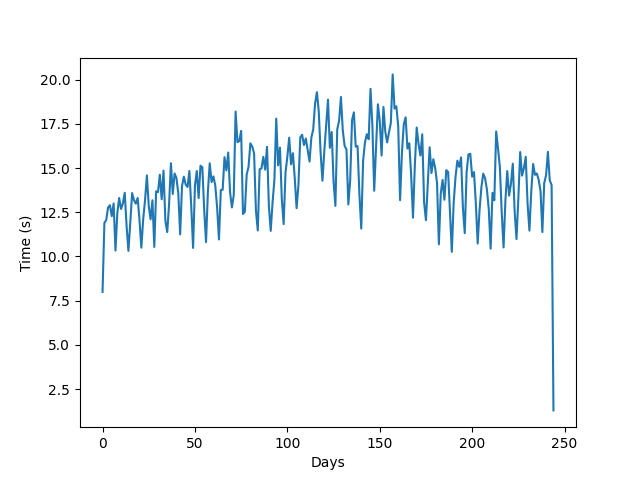
\includegraphics[width=0.7\linewidth]{image/time}
	\caption{زمان‌ به روز رسانی وضعیت امتیاز‌ها برای هر روز}
	\label{fig:time_proposed}
\end{figure}

شکل \ref{fig:betachange} درصد تغییرات آدرس‌ها در بین تکه‌های مختلف نسبت به کل آدرس‌ها با توجه به مقدرا $\beta$ را نشان می‌دهد. هر چه این مقدار به $1$ نزدیک  تر باشد، امتیاز آدرس‌ها سریع‌تر تغییر می‌کند.

\begin{figure}
	\centering
	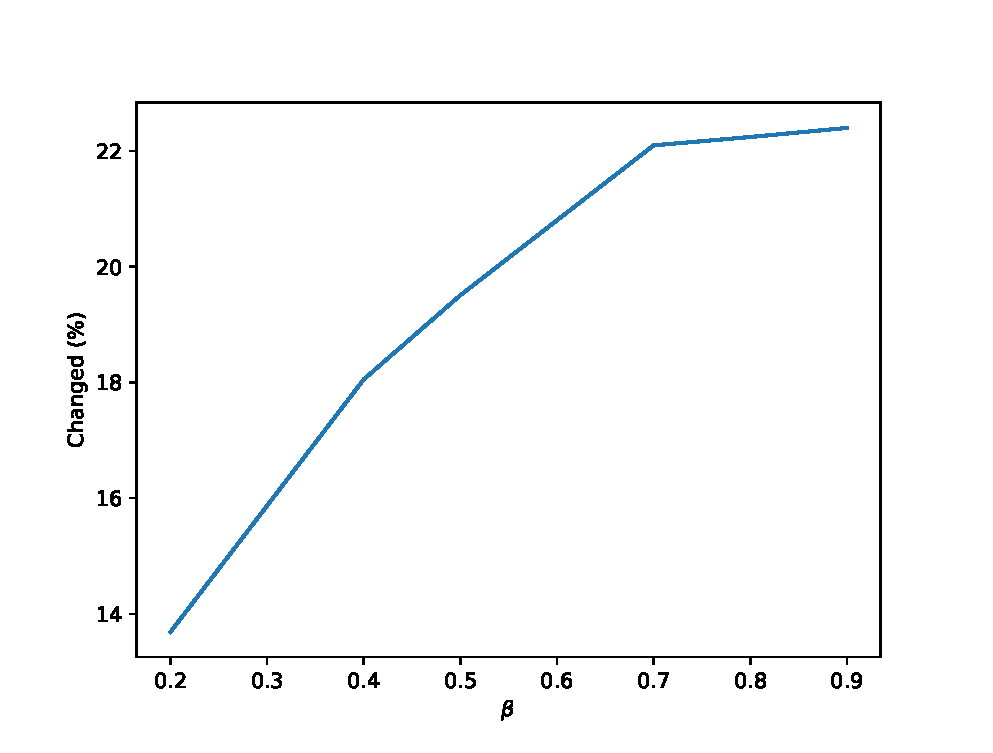
\includegraphics[width=0.7\linewidth]{image/beta_change}
	\caption{درصد آدرس‌های تغییر کرده در بین تکه‌های مختلف به تعداد کل آدرس‌ها با توجه به اندازهٔ $\beta$}
	\label{fig:betachange}
\end{figure}



\subsubsection{بحث و نتیجه‌گیری}

در روش ارائه شده سعی شده است که بدون نیاز به استفاده از پروتکل و ابزار‌های پیچیده، با حذف فیلتر بلوم بهره‌گیری از معیار ‌$K$-گمنامی و قرار دادن آدرس‌هایی با احتمال درخواست یکسان، در یک دسته به سطح بالاتری از امنیت نسبت به فیلتر بلوم دست پیدا شود. همچنین در این روش تعیین پهنای باند مصرفی کاملا در اختیار کاربر سبک است و کاربر سبک می‌تواند با سطح امنیت مورد نظرش این مقدار را تعیین کند.

مقدار $\beta$ باید پیش از راه‌اندازی پروتکل تعیین شود. هر چه این مقدار بیش‌تر باشد، تغییرات آدرس‌ها در تکه‌ها سریع‌تر بوده و به گره کامل متخاصم امکان می‌دهد که با اشتراک‌گیری، آدرس مورد نظر کاربر را تشخیص دهد، از طرف دیگر اگر مقدار آن کم باشد باعث می‌شود که آدرس‌هایی که در یک تکه قرار گرفته‌اند در حال حاضر مقدار امتیاز مشابهی نداشته باشند در نتیجه، طبق فرمول \eqref{eq:9} آنتروپی آدرس‌ها در یک تکه کاهش پیدا می‌کند. در نتیجه باید بررسی‌های بیش‌تری برای انتخاب $\beta$ انجام گیرد.

\begin{xltabular}{\textwidth}{|r|X|}
	\caption{
		مقایسهٔ  امنیت، پهنای باند و پردازش سمت گره کامل برای روش ارائه شده
		\label{table:Proposed}}\\
	\hline
	\textbf{معیار} & \textbf{توضیحات} \\
	\hline
	{%
		امنیت
	}&{%
		امکان تعیین آدرس‌های پوششی به صورت هوشمندانه و به مقدار دلخواه، استقلال بین درخواست‌های کاربر و دشواری ایجاد پیوند بین درخواست‌های وی، مقاوم در برابر تحلیل بسامد استفاده از آدرس، عدم نیاز به تجهیزات سخت‌افزاری و نرم‌افزاری پیچیده و امکان راه‌اندازی ساده‌ٔ یک گره کامل و در نتیجه کاهش نیاز به اعتماد به گره‌های محدود جهت دریافت خدمات
	}\\
	\hline
	{%
		پهنای باند مصرفی
	}&{%
		پهنای باند مصرفی قابل تنظیم که تنها شامل تراکنش‌های اصلی به علاوه تراکنش‌های پوششی و اثبات مرکل آن‌ها است.
	}\\
	\hline
	{%
		پردازش سمت کاربر کامل
	} & {%
	با توجه به شکل \ref{fig:time_proposed} به ازای به روز رسانی هر روزانه، زمان زیادی صرف نمی‌شود.
}\\
\hline
\end{xltabular}





		% فصل چهارم: ارائهٔ روش
% !TeX root=../main.tex
\chapter{
	نتیجه‌گیری و کار‌های آینده}
%\thispagestyle{empty} 
\label{chap:future}

در روش ارائه شده سعی شده است که بدون نیاز به استفاده از پروتکل و ابزار‌های پیچیده، با حذف فیلتر بلوم و بهره‌گیری از معیار ‌$K$-گمنامی و قرار دادن آدرس‌هایی با احتمال درخواست یکسان، در یک دسته به سطح بالاتری از امنیت نسبت به فیلتر بلوم دست پیدا شود. همچنین در این روش تعیین پهنای باند مصرفی کاملا در اختیار کاربر سبک است و کاربر سبک می‌تواند با سطح امنیت مورد نظرش این مقدار را تعیین کند.

در این پایان‌نامه با فرض این‌که احتمال پرسمان اطلاعات مربوط به هر آدرس $a_n$، به شرطی که مربوط به یک گره کامل نباشد، متناسب است با احتمال استفاده از آن آدرس در شبکه بیت‌کوین پروتکل طراحی شده است. هرچند که این فرض،‌ دور از ذهن نیست اما لازم است که صحت آن از طریق شبیه‌سازی سنجیده شود. به این منظور، در این  پژوهش سعی شد که یک نرم افزار 
\gls{Bitcoin-core}
راه‌اندازی شده تا درخواست‌های گره‌های سبک، که از فیلتر بلوم استفاده می‌کنند، ثبت شود. همچنین سعی شد که با بهره‌گیری از ایدهٔ پایان‌نامهٔ \cite{Nick2015}، که برای کشف آدرس‌های اصلی فیلتر بلوم \lr{PubKey} و \lr{PubKeyHash} آدرس‌های بیت‌کوین را در فیلتر‌های بلوم آزمایش کرده بود، به آدرس‌های اصلی فیلترهای دریافت شده پی برده شود. در کنار این، یک سرور
الکترام‌ایکس\LTRfootnote{\lr{ElectrumX}}
نیز راه‌اندازی شد تا به صورت مستقیم، بدون استفاده از فیلتر بلوم، نرخ درخواست از طرف کیف‌پول‌های بیت‌کوین الکرترام ثبت شود. اما متاسفانه، به خاطر محدود بودن پهنای باند و الزام استفاده از شبکهٔ 
\gls{Tor}
به خاطر نداشتن آدرس IP استاتیک، فرصت نشد که گره‌ کامل راه‌اندازی شده به صورت کامل به شبکه شناسانده شود و تعداد درخواست‌های قابل توجهی دریافت نماید. از این رو لازم است که برای درستی سنجی فرض انجام شده در آینده شبیه‌سازی‌ گسترده طولانی مدتی انجام گیرد. 

پارامتر $\beta$ در این پروتکل و هچنین مرز بین تکه‌ها در امنیت پروتکل تاثیر مستقیمی دارد. لازم است که در آینده مقدار مشخصی برای این پارامتر محاسبه شود. روش محاسبهٔ امتیازها در این پایان‌نامه یک روش 
\gls{Naive} 
محسوب می‌شود که امکان اجماع همه گره‌ها بر روی امتیاز نهایی را فراهم نموده است. به نظر می‌رسد که با بررسی بیشتر امکان بهره‌گیری از ابزار‌ها و متدهای پیشرفته‌تری برای محاسبهٔ امتیا‌ز‌ها وجود خواهد داشت.

		% فصل پنجم: کار‌های آینده و نتیجه‌گیری
%% !TeX root=../main.tex
\chapter{
	نتیجه‌گیری و کار‌های آینده}
%\thispagestyle{empty} 
\label{chap:future}

در روش ارائه شده سعی شده است که بدون نیاز به استفاده از پروتکل و ابزار‌های پیچیده، با حذف فیلتر بلوم و بهره‌گیری از معیار ‌$K$-گمنامی و قرار دادن آدرس‌هایی با احتمال درخواست یکسان، در یک دسته به سطح بالاتری از امنیت نسبت به فیلتر بلوم دست پیدا شود. همچنین در این روش تعیین پهنای باند مصرفی کاملا در اختیار کاربر سبک است و کاربر سبک می‌تواند با سطح امنیت مورد نظرش این مقدار را تعیین کند.

در این پایان‌نامه با فرض این‌که احتمال پرسمان اطلاعات مربوط به هر آدرس $a_n$، به شرطی که مربوط به یک گره کامل نباشد، متناسب است با احتمال استفاده از آن آدرس در شبکه بیت‌کوین پروتکل طراحی شده است. هرچند که این فرض،‌ دور از ذهن نیست اما لازم است که صحت آن از طریق شبیه‌سازی سنجیده شود. به این منظور، در این  پژوهش سعی شد که یک نرم افزار 
\gls{Bitcoin-core}
راه‌اندازی شده تا درخواست‌های گره‌های سبک، که از فیلتر بلوم استفاده می‌کنند، ثبت شود. همچنین سعی شد که با بهره‌گیری از ایدهٔ پایان‌نامهٔ \cite{Nick2015}، که برای کشف آدرس‌های اصلی فیلتر بلوم \lr{PubKey} و \lr{PubKeyHash} آدرس‌های بیت‌کوین را در فیلتر‌های بلوم آزمایش کرده بود، به آدرس‌های اصلی فیلترهای دریافت شده پی برده شود. در کنار این، یک سرور
الکترام‌ایکس\LTRfootnote{\lr{ElectrumX}}
نیز راه‌اندازی شد تا به صورت مستقیم، بدون استفاده از فیلتر بلوم، نرخ درخواست از طرف کیف‌پول‌های بیت‌کوین الکرترام ثبت شود. اما متاسفانه، به خاطر محدود بودن پهنای باند و الزام استفاده از شبکهٔ 
\gls{Tor}
به خاطر نداشتن آدرس IP استاتیک، فرصت نشد که گره‌ کامل راه‌اندازی شده به صورت کامل به شبکه شناسانده شود و تعداد درخواست‌های قابل توجهی دریافت نماید. از این رو لازم است که برای درستی سنجی فرض انجام شده در آینده شبیه‌سازی‌ گسترده طولانی مدتی انجام گیرد. 

پارامتر $\beta$ در این پروتکل و هچنین مرز بین تکه‌ها در امنیت پروتکل تاثیر مستقیمی دارد. لازم است که در آینده مقدار مشخصی برای این پارامتر محاسبه شود. روش محاسبهٔ امتیازها در این پایان‌نامه یک روش 
\gls{Naive} 
محسوب می‌شود که امکان اجماع همه گره‌ها بر روی امتیاز نهایی را فراهم نموده است. به نظر می‌رسد که با بررسی بیشتر امکان بهره‌گیری از ابزار‌ها و متدهای پیشرفته‌تری برای محاسبهٔ امتیا‌ز‌ها وجود خواهد داشت.

		% فصل پنجم: بحث و نتیجه‌گیری

% مراجع
% اگر از استیل‌های natbib استفاده می‌کنید باید دو خط را در فایل commands.tex تغییر دهید.
\pagestyle{empty}
{
\small
\onehalfspacing
\bibliographystyle{plain-fa} % or plainnat-fa for author-date
\bibliography{./tex/MyReferences}
}

\pagestyle{fancy}

% \appendix
% فصلهای پس از این قسمت به عنوان ضمیمه خواهند آمد.

% دستورات لازم برای تبدیل «فصل آ» به «پیوست آ» در فهرست مطالب
\addtocontents{toc}{
    \protect\renewcommand\protect\cftchappresnum{\appendixname~}%
    \protect\setlength{\cftchapnumwidth}{\mylenapp}}
    
\let\Chapter\chapter
% دستورات لازم برای شماره‌گذاری صفحات پیوست‌ها بشکل آ-۱ (فعلا با glossaries سازگار نیست)
%\pretocmd{\chapter}{
%  \clearpage
%  \pagenumbering{arabic}
%  \renewcommand*{\thepage}{\rl{\thechapter-\arabic{page}}}}{}{}
%%%%%%%%%%%%%%%%%%%%%%%%%%%%%%%%%%%%%
    

%% !TeX root=../main.tex

\chapter{اتصال گره سبک به شبکهٔ همتابه‌همتای بیت‌کوین}
\label{app:p2p}
%\thispagestyle{empty}
در این پیوست نحوهٔ اتصال یک گره سبک به شبکهٔ همتا‌به‌همتای بیت‌کوین توضیح داده می‌شود. تمام  ارتباطات همتا‌به‌همتا در بیت‌کوین در بستر TCP برقرار می‌شود و تمام پیام‌ها از قالب یکسانی پیروی می‌کنند. رشتهٔ آغازین پیام‌ها و مقدار پیش‌فرض شمارهٔ درگاه با توجه به اینکه پیام در شبکهٔ اصلی، تست یا در حالت تست رگرسیون استفاده می‌شود تفاوت می‌کند. جدول \ref{table:PortandString} این مقادیر را نشان می‌دهد. یک گره می‌تواند از شمارهٔ درگاهی متفاوت در یک شبکه استفاده نماید.



\begin{xltabular}{\textwidth}{|c|c|c|X|}
	\caption{شبکه‌های مختلف بیت‌کوین\label{table:PortandString}}\\
	\hline
	\textbf{شبکه} & \textbf{درگاه پیش‌فرض} & \textbf{رشته‌ٔ آغازین} & \textbf{توضیحات} \\
	\hline \hline 
	اصلی & 8333 & \lr{\texttt{0xf9beb4d9}} & {%
		شبکهٔ اصلی بیت‌کوین.
	}\\
	\lr{Mainnet} & & & {%
		در این شبکه بیت‌کوین دارای ارزش واقعی است.
	} \\
	\hline
	تست & 18333 & \lr{\texttt{0x0b110907}} & {%
		شبکهٔ آزمایشی بیت‌کوین
	}\\
	\lr{Testnet} & & & {%
		برای توسعه دهندگان بهتر و کم هزینه‌ تر است که از شبکهٔ آزمایشی بیت‌کوین استفاده کنند. چرا که بیت‌کوین‌ در آن دارای ارزش واقعی نیست.
	} \\
	\hline
	تست رگرسیون & 18444 & \lr{\texttt{0xfabfb5da}} & {%
		حالت تست رگرسیون
	}\\
	\lr{Regtest} & & & {%
		گاهی در توسعه یک کاربرد نیازی نیست که با گره‌های تصادفی در ارتباط باشیم یا بلوک‌های تصادفی تولید شده را بررسی کنیم. در این شرایط از حالت تست رگرسیون بیت‌کوین استفاده می‌کنیم. در این حالت می‌توان محیط را کنترل کرد و تعیین کرد که چه زمانی یک بلوک جدید ساخته شود.
	} \\
	\hline
	
	
\end{xltabular}


علاوه بر این تمام پیام‌های شبکه‌ٔ همتا‌به‌همتای بیت‌کوین شامل سرایندی یکسان هستند که قالب این سرایند مطابق جدول \ref{table:p2pheader} است.

\begin{xltabular}{\textwidth}{|c|X|}
	\caption{قالب سرایند تمام‌ پیام‌ها در شبکهٔ همتا‌به‌همتای بیت‌کوین \label{table:p2pheader}}\\ \hline
	\textbf{نام} & {\textbf{توضیحات} } \\
	\hline \hline
	\lr{start string}&{%
		بایت‌هایی که در جدول \ref{table:PortandString} توضیح داده شد که نشان دهندهٔ شبکه‌ای است که این پیام در آن تولید شده است.
	}\\
	\hline
	
	\lr{command name} & {%
		رشته‌ای در استاندارد 
		%		اَسکی
		\gls{ASCII}\LTRfootnote{ASCII}
		است که مشخص می‌کند چه نوع پیامی در 		
		\gls{Payload}\LTRfootnote{Payload}
		قرار گرفته است. اندازهٔ این قسمت ۱۲ کاراکتر است و بایت‌های بعد از نام پیام برابر صفر (\texttt{0x00}) خواهند بود. به عنوان مثال برای پیام \texttt{Version} خواهیم داشت:
		\lr{\texttt{version\textbackslash0\textbackslash0\textbackslash0\textbackslash0\textbackslash0}}.
	}\\
	\hline
	
	\lr{payload size} & {%
		اندازه بایت‌های پیام داخل پایه‌بار را مشخص می‌کند. حداکثر تعداد بایت‌ مجاز در پایه‌بار ۳۲ مگابایت‌ (\lr{‍‍``MAX\_SIZE''}) است. پیام‌های بزرگ‌تر از این مقدار دورانداخته می‌شوند. پیام‌هایی مانند \texttt{VerAck}   بدون پایه‌بار هستند.
	}\\
	\hline
	
	\lr{checksum} & {%
		چهار بایت اول حاصل 
		\lr{SHA256(SHA256(payload))}
		است. اگر پایه‌بار خالی باشد، مانند پیام‌های \texttt{VerAck} و \texttt{GetAddr}، مقدار این بخش برابر 
		\lr{\texttt{0x5df6e0e2}}
		بوده که معادل 
		\lr{SHA256(SHA256(
			\rl{رشتهٔ خالی}
			))}
		است.
	}\\
	\hline
	
\end{xltabular}  

\section{یافتن همتا}

اولین گامی که هر گره در شبکهٔ همتا‌به‌همتای بیت‌کوین انجام می‌دهد، یافتن گره‌های (همتا‌های) دیگر و اتصال به آن‌ها است. از آن‌جایی که یک گره در زمان راه اندازی، آدرس آی‌پی گره‌های کامل فعال را ندارد، از یک یا چند سرور 
\LTRfootnote{\lr{Domain Name System}}\lr{DNS} 
که آدرس‌ آن‌ها در کد بیت‌کوین‌جی از پیش قرارگرفته است پرسمان انجام می‌دهد. پاسخ دریافت شده شامل آدرس یک یا چند گره کامل است که ارتباطات ورودی را قبول می‌کنند. علاوه بر این تعدادی آدرس گره کامل در هر ورژن از کدهای بیت‌کوین‌جی قرار دارد که در زمانی که آن ورژن مشخص منتشر می‌شده فعال بوده‌اند. 
\subsubsection{اتصال به همتا}
بعد از آن‌که کاربر جدید آدرس آی‌پی یک یا چند گره کامل را بدست آورد، برای آن گره‌(ها) پیام \texttt{version} را ارسال می‌کند. این پیام برای ایجاد ارتباط ارسال می‌شود و شامل اطلاعاتی از گره ارسال کننده است. این اطلاعات در جدول \ref{table:VersionMessage} توضیح داده شده است. گره دریافت کننده نیز یک پیام \texttt{version} را که شامل اطلاعات خودش است، ارسال می‌کند. هر دو گره به محض دریافت پیام \texttt{version} پیام \texttt{verack} را برای گره مقابل ارسال می‌نماید. پیام \texttt{verack} بدون
%پایه‌بار\RTLfootnote{Payload}
\gls{Payload}
است و به گره دریافت کننده اطلاع می‌دهد که آماده دریافت پیام‌‌های بعدی است.


\begin{xltabular}{\textwidth}{|c|X|}
	\caption{
		قسمت‌های پیام \texttt{version} در شبکه همتا‌به‌همتای بیت‌کوین
		\label{table:VersionMessage}}\\
	\hline
	\textbf{نام} & {\centering
		\textbf{توضیحات}		
	} \\
	\hline
	\hline
	\lr{version} & {
		بالاترین نسخهٔ پروتکلی که توسط گره ارسال کننده شناخته می‌شود.	در زمان نگارش این پایان‌نامه، بالاترین نسخه پروتکل بیت‌کوین 70015 است که در سال ۲۰۱۷ منتشر شده است.
	} \\
	\hline
	\lr{services} & {
		خدماتی که گره ارسال‌کننده پشتیبانی می‌کند را مشخص می‌کند. برای گره‌های سبکی مثل بیت‌کوین‌جی، مقدار آن برابر \texttt{0x00} است.
	} \\
	\hline
	\lr{timestamp} & {
		%		ساعت یونیکس\RTLfootnote{\lr{Unix time}} 
		\gls{Unix time}\LTRfootnote{\lr{Unix time}}
		با توجه به ساعت گره ارسال کننده در زمان ارسال پیام.
	} \\
	\hline
	\lr{addr\_recv services} & {
		سرویس‌هایی که از دید گره ارسال‌کننده، توسط گره گیرنده پشتیبانی می‌شود. فرمت نمایش آن مانند قسمت services است. اگر گره ارسال‌کننده، بیت‌کوین‌جی باشد، همیشه به صورت پیش‌فرض مقدار این قسمت را برابر \texttt{0x00} قرار می‌دهد.
	} \\
	\hline
	\lr{addr\_recv port} & {
		شماره پورت گره گیرنده از دید گره ارسال‌کننده.
	}\\
	\hline
	\lr{addr\_trans services} & {
		خدماتی که گره ارسال‌کننده پشتیبانی می‌کند را مشخص می‌کند. یکسان با قسمت services باید باشد.
	}\\
	
	\hline
	\lr{addr\_trans IP address} & {
		آدرس آی‌پی گره ارسال کننده.
	}\\
	
	\hline
	\lr{addr\_trans port} & {
		شماره پورت گره ارسال کننده.
	}\\
	
	\hline
	\lr{nonce} & {
		تک‌شمار، یک عدد تصادفی است که اگر یک گره،‌ یک پیام با تک‌شماری مشابه با تک‌شمار ارسالی دریافت کرد، ارتباط را قطع نماید. (قسمت تک‌شمار در نسخهٔ \lr{$0.1.6$} بیت‌کوین اضافه شده و هدفش آن است که گره متوجه شود که به خودش متصل نشده باشد)
		\LTRfootnote{  \lr{\url{https://github.com/bitcoin/bitcoin/commit/cc0b4c3b62367a2aebe5fc1f4d0ed4b97e9c2ac9}}}.
	}\\
	\hline
	\lr{user\_agent bytes} & {
		تعداد بایت‌هایی که پیام قسمت \lr{user\_agent} (قسمت بعدی) استفاده کرده است.
	}\\
	
	\hline
	\lr{user\_agent} & {
		نوع برنامه کاربر را معین می‌کند. مثلا:
	}\\
	
	&  {%
		۱. بیت‌کوین‌جی: 
		\lr{/bitcoinj:1.0/MultiBit:1.0(Windows)/}} \\
	&  {%
		۲. هستهٔ بیت‌کوین (گره کامل): 
		\lr{/Satoshi:0.20.0/(70015)/}} \\
	
	\hline
	\lr{start\_height} & {
		ارتفاع بهترین زنجیره‌ بلوکی گره ارسال کننده در این قسمت قرار گرفته می‌شود. در صورتی که کاربر SPV باشد، ارتفاع بهترین زنجیره سرایند بلوک‌‌ها قرار داده می‌شود.
	}\\
	
	\hline
	\lr{relay} & {
		قرار دادن این بخش در پیام اختیاری است. این بخش در \cite{Hearn2013} به همراه پیشنهاد استفاده از فیلتر بلوم در بیت‌کوین معرفی شده است. مقدار آن صحیح (\texttt{0x01}) یا غلط (\texttt{0x00}) است. در صورتی که صحیح باشد، یا از آن استفاده نشود، تغییری در پروتکل ایجاد نمی‌شود. ولی در صورتی که غلط باشد، قبل از آن‌که کاربر ارسال کننده، پیام‌های \texttt{filterload} و \texttt{filterclear} را ارسال کرده باشد، هیچ پیام \texttt{inv} یا \texttt{tx} به آن ارسال نمی‌شود. این کار باعث می‌شود که در فاصلهٔ زمانی انجام 
		%		دستداد \RTLfootnote{Handshake}
		\gls{Handshake}\LTRfootnote{Handshake}
		(ارسال پیام \texttt{version}) و فرستادن فیلتر بلوم، کاربر سبک تحت سیل پیام‌های گره‌کامل قرار نگیرد. 
	}\\
	
	
	\hline
\end{xltabular}

زمانی که اتصال با یک گره کامل برقرار شد، پیام \texttt{getaddr} برای گره کامل فرستاده می‌شود تا آدرس آی‌پی گره‌های کامل فعالی که گره دریافت‌کننده به آن‌ها متصل است در قالب پیام \texttt{addr} برای گره فرستنده ارسال شود. گره فرستنده همتا‌های فعال خودش را نیز در قالب پیام \texttt{addr} برای گره کامل گیرنده ارسال می‌کند.

\section{هم‌گام سازی گره سبک}
از این قسمت به بعد تنها به بررسی فعالیت‌های گره سبک در شبکه می‌پردازیم و هم‌گام‌سازی دیگر گره‌های شبکه مورد بررسی قرار نمی‌گیرند. کاربر سبک بعد از اتصال اولیه به یک گره کامل، نیاز دارد که سرایند بلوک‌های زنجیرهٔ بلوکی را دریافت نماید به این کار 
%هم‌گام‌سازی \RTLfootnote{Synchronization}
\gls{Synchronization}
گفته می‌شود. همان‌طور که گفته شد کاربر سبک به جای ذخیره‌سازی و تصدیق تمام زنجیرهٔ بلوکی،‌ تنها سرایند آن را ذخیره می‌کند. حجم سرایند یک بلوک $80$ بایت است. در گره‌های کامل، که می‌خواهند تمام زنجیره بلوکی را دریافت نمایند، این فرایند به دو صورت
%«ابتدا-بلوک\RTLfootnote{Blocks-First}»
«\gls{Blocks-First}»
یا
«\gls{Headers-First}»
قابل انجام است که در این‌جا به توضیح آن‌ها پرداخته نمی‌شود. گره سبک در گام اول هم‌گام‌سازی لازم است که 
%بهترین سراید زنجیرهٔ بلوکی \RTLfootnote{\lr{Best header chain}} 
\gls{Best header chain}
را دانلود کند. سرایند زنجیرهٔ بلوکی، زنجیره‌ای از سرایند بلوک‌ها است که هر کدام از سرایند‌ها به سرایند بلوک قبل خود اشاره می‌کند. بهترین سرایند زنجیرهٔ بلوکی، زنجیره‌ای است که دشوارترین بازآفرینی را داشته باشد. 

گره سبک برای دریافت سرایند زنجیرهٔ بلوکی، پیام \texttt{getheaders} را برای گره کاملی (گره هم‌گام‌ساز) که می‌خواهد با آن همگام شود ارسال می‌کند. جدول \ref{table:GetHeadersMessage} بخش‌های مختلف این پیام را توضیح می‌دهد و شکل \ref{fig:getheaders} مثالی از یک پیام \texttt{getheaders} است که گره سبک برای اولین‌بار برای گره هم‌گام‌ساز ارسال می‌کند.



\begin{xltabular}{\textwidth}{|c|X|}
	\caption{
		قسمت‌های پیام \texttt{getheaders} در شبکه همتا‌به‌همتای بیت‌کوین
		\label{table:GetHeadersMessage}}\\
	\hline
	\textbf{نام} & {\textbf{توضیحات}} \\
	\hline \hline
	\lr{version} & {%
		شماره‌ٔ نسخه‌ٔ پروتکل. شبیه آنچه در پیام \texttt{version} ارسال شد.
	} \\
	
	\hline
	
	\lr{hash count} & {%
		تعداد چکیده‌هایی که در بخش بعدی پیام قرار می‌گیرند، در این قسمت تعیین می‌شوند. محدودیتی در تعداد چکیده‌های ارسالی نیست. اما اندازه کل پیام باید کمتر از \lr{‍‍``MAX\_SIZE''} (۳۲ مگابایت) باشد.
	} \\
	\hline
	
	
	\lr{block header hashes} & {%
		چکیدهٔ یک یا چند سرایند بلوکی که گره ارسال کننده آن‌ها را در حافظهٔ خود دارد. ترتیب چکیده‌ها از بالاترین ارتفاع بلوک (جدید‌ترین) به پایین‌ترین ارتفاع است. به این ترتیب به گره دریافت‌کننده‌ٔ پیام این امکان داده می‌شود که جدیدترین چکیدهٔ سرایندی که با هم مشترک هستند را پیدا کند. اگر گره سبکش تازه راه‌اندازی شده‌ باشد در این قسمت، چکیدهٔ بلوک جنسیس (\lr{6fe2…0000}) را که در نرم‌افزارش از ابتدا وجود داشته است، قرار می‌دهد.
	} \\
	\hline
	
	\lr{stop hash} & {%
		این قسمت چکیدهٔ آخرین بلوکی است که گره ارسال‌کننده می‌خواهد دریافت کند. با صفر قراردادن آن، طولانی‌ترین پاسخ ممکن از گره کامل تقاضا می‌شود. حداکثر تعداد سرایندی که گره کامل دریافت کنندهٔ این پیام پاسخ می‌دهد، $2000$ سرایند است. برای دریافت بیشتر از این مقدار، این پیام در چند نوبت ارسال می‌شود
	}\\
	\hline
	
\end{xltabular}

\begin{figure}[h]
	\centering
	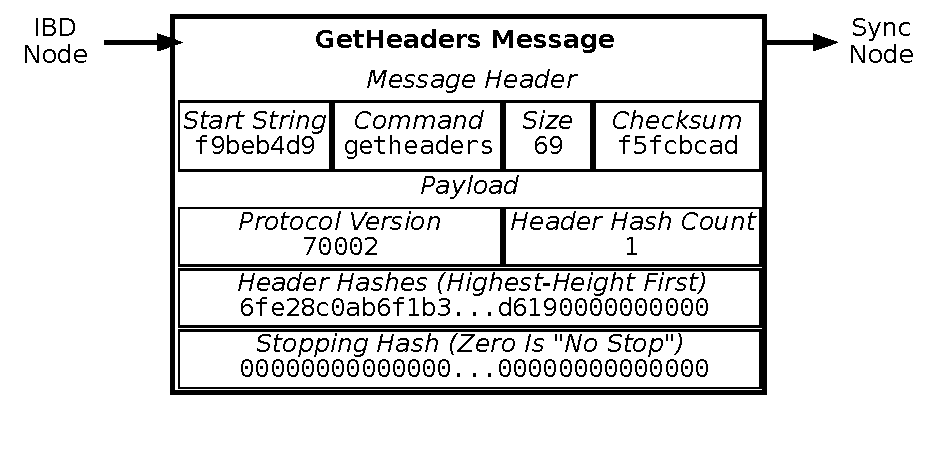
\includegraphics[width=0.7\linewidth]{image/getheaders}
	\caption{مثالی از پیام \texttt{getheaders} در همگام‌سازی اولیهٔ یک گره جدید}
	\label{fig:getheaders}
\end{figure}


گره هم‌گام‌ساز در پاسخ به پیام \texttt{getheaders} در شکل \ref{fig:getheaders} دنبال بلوکی با چکیده مشخص شده می‌گردد و می‌یابد که این بلوک برابر بلوک شمارهٔ صفر (بلوک جنسیس) است. به این ترتیب $۲۰۰۰$ سرایند بلوک را که از بلوک شمارهٔ یک آغاز می‌شوند در قالب پیام \texttt{headers} برای گره درخواست دهنده ارسال می‌کند. قالب این پیام در جدول \ref{table:HeadersMessage} مشخص شده‌ است. شکل \ref{fig:headers} مثالی از پیام بازگردانده شده توسط گره هم‌گام‌ساز است.

\begin{table}[!h]
	\centering
	\caption{
		قسمت‌های پیام \texttt{headers} در شبکه همتا‌به‌همتای بیت‌کوین
		\label{table:HeadersMessage}}
	\begin{tabular}{|c|r|}
		\hline
		\textbf{نام} & {\textbf{توضیحات}} \\
		\hline \hline
		
		\lr{count} & {%
			تعداد سرایند‌های بلوک قرار گرفته در بخش بعدی این پیام. (حداکثر $2000$)
		} \\
		\hline
		
		\lr{headers} & {%
			سرایند‌ بلوک‌ها در این قسمت قرار می‌گیرند.
		} \\
		\hline
	\end{tabular}
\end{table}

\begin{figure}[!h]
	\centering
	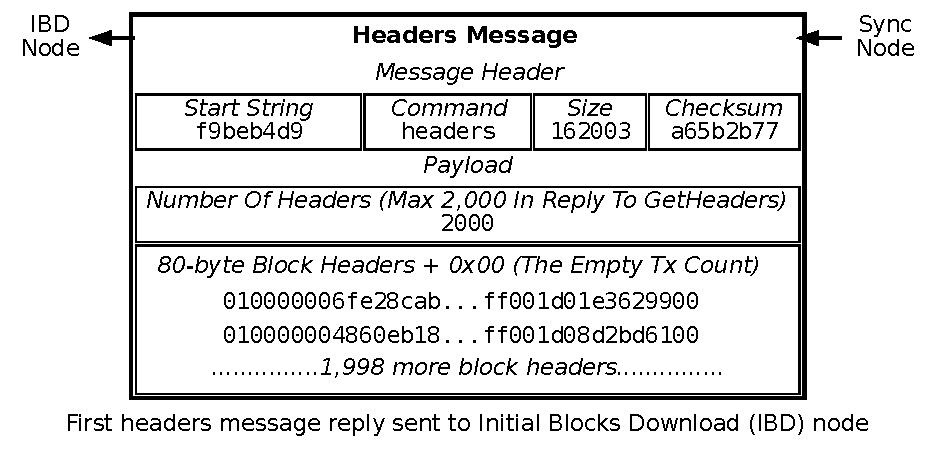
\includegraphics[width=0.7\linewidth]{image/headers}
	\caption{مثالی از پیام \texttt{headers} در همگام‌سازی اولیهٔ یک گره جدید}
	\label{fig:headers}
\end{figure}

وقتی گره سبک پاسخ شکل \ref{fig:headers} را دریافت کرد، فورا صحت آن را بررسی کرده و مجددا پیام  \texttt{getheaders} جدیدی برای گره همگام‌ساز برای گرفته باقیمانده سرایند‌ها ارسال می‌کند. این فرایند تا گرفتن کامل سرایند‌ها ادامه پیدا می‌کند. در زمان نوشتن این پایان‌نامه، حجم تمام سرایند‌های زنجیرهٔ بلوکی ۵۰ مگابایت است. پس از اتمام دانلود سرایند‌های زنجیرهٔ  بلوکی، گره سبک آخرین پیام \texttt{getheaders} را برای چند همتای دیگر ارسال کرده و پاسخ آن‌ها را با پاسخ گره هم‌گام‌ساز ابتدایی مقایسه می‌کند. به این ترتیب مطمئن می‌شود که بهترین سرایند زنجیرهٔ بلوکی را دریافت کرده است. 

\section{انتشار}

زمانی که گره کامل یک بلوک جدید را دریافت می‌کند، پیام \texttt{inv} را برای همهٔ همتا‌هایش (چه گره کامل چه گره سبک) ارسال می‌کند. پیام ارسال شده دارای یک 
%مدخل فهرست \RTLfootnote{Inventory} 
\gls{Inventory}
مربوط به بلوک جدید است. یک مدخل فهرست، شامل یک علامت نوع داده و یک  چکیده داده به عنوان مشخص‌کنندهٔ آن است. داده می‌تواند انواع مختلفی داشته باشد، به عنوان نمونه، علامت تراکنش
\lr{``MSG\_TX''}
و علامت بلوک
\lr{``MSG\_BLOCK''}
است.
به صورت کلی مدخل فهرست به وجود تراکنش‌ها یا بلوک‌هایی برای دانلود اشاره می‌کند. جدول \ref{table:InvMessage} قسمت‌های مختلف پیام \texttt{inv} را شرح می‌دهد. 

\begin{xltabular}{\textwidth}{|c|X|}
	\caption{
		قسمت‌های پیام \texttt{inv} در شبکه همتا‌به‌همتای بیت‌کوین
		\label{table:InvMessage}}\\
	\hline
	\textbf{نام} & {\textbf{توضیحات}} \\
	\hline \hline
	
	\lr{compactSize uint} & {%
		تعداد مدخل‌های فهرست. 
	}\\
	\hline
	
	\lr{inventory} & {%
		یک یا چند مدخل فهرست. حداکثر تعداد آن می‌تواند $50000$ باشد. به عنوان مثال محتوای این قسمت از پیام برای اطلاع‌رسانی بلوک ارتفاع 
		$645747$\LTRfootnote{\url{https://blockchair.com/bitcoin/block/645747}}
		به گره‌های همتا به این صورت است: 
	}\\
	
	&{%
		علامت نوع داده:
		\lr{MSG\_BLOCK}
	}\\
	
	&{%
		مشخص‌کنندهٔ داده (چکیده):
		\lr{\texttt{0x333ab9f10d...0000000000}}
	}\\
	
	\hline
	
\end{xltabular}

گره سبک بعد از دریافت این پیام، یک پیام \texttt{getdata} برای گره کامل می‌فرستد. در این پیام درخواست می‌کند که با توجه به فیلتر بلومی که پیش‌تر در اختیار گره کامل گذاشته بوده، تراکنش‌هایی از بلوک جدید را، که در آن فیلتر صدق می‌کنند برای وی بفرستد. ساختار پیام \texttt{getdata} شبیه \texttt{inv} است. با این تفاوت که علامت نوع داده،‌ اطلاعاتی است که گره ارسال کننده این پیام از گره دریافت‌کننده درخواست می‌کند. 
در این کاربرد، گره سبک علامت \lr{‍‍‍``MSG\_FILTERED\_BLOCK''}  را در کنار چکیده‌ٔ بلوک مورد نظر در پیام قرار می‌دهد و برای گره کامل ارسال می‌کند. به این ترتیب گره کامل تراکنش‌هایی که حداقل یک آدرس آن‌ها در فیلتر بلوم صدق می‌کنند را در کنار اثبات مرکل آن‌ها برای گره سبک ارسال می‌کند.
پاسخ در قالب یک پیام \texttt{merkleblock} که شامل اثبات مرکل وجود تراکنش‌های مرتبط در بلوک است و تعداد صفر یا چند پیام \texttt{tx} را که خود تراکنش‌ها هستند خواهد بود. 
		% پیوست اول: آشنایی مقدماتی با لاتک
%% !TeX root=../main.tex

\chapter{‌جدول، نمودار و الگوریتم در لاتک}
\label{app:latex:more}
%\thispagestyle{empty}

در این بخش نمونه مثالهایی از جدول، شکل، نمودار، الگوریتم و معادلات ریاضی را در لاتک خواهیم دید.
دقت کنید که در پایان‌نامه‌ها و مقالات، باید قاعدهٔ «ارجاع به جلو%
\LTRfootnote{Forward Referencing}»
رعایت شود؛ یعنی ابتدا در متن به شمارهٔ شکل، جدول یا معادله اشاره شود و بعد از آن (زیر آن) خود شکل، جدول یا معادله رسم شود. (توضیحات بیشتر در قسمت
\ref{sec:floatObjs}).

\section{جدول}
دستور اصلی برای رسم جدول در لاتک 
\verb|tabular|
می‌باشد که جدول
\eqref{tab:motionModels}
با استفاده از آن کشیده شده است؛ در
\verb|tabular|
عرض جدول برابر با مجموع عرض ستون‌ها و حداکثر مساوی عرض متن است.
\begin{table}[ht]
\caption{مدلهای تبدیل.}
\label{tab:motionModels}
\centering
\onehalfspacing
\begin{tabular}{|r|c|l|r|}
	\hline نام مدل & درجه آزادی & تبدیل مختصات & توضیح \\ 
	\hline انتقالی & ۲ & $\begin{aligned} x'=x+t_x \\ y'=y+t_y \end{aligned}$  &  انتقال دوبعدی\\ 
	\hline اقلیدسی & ۳ & $\begin{aligned} x'=x\cos\theta - y\sin\theta+t_x \\ y'=x\sin\theta+y\cos\theta+t_y \end{aligned}$  &  انتقالی+دوران \\ 
	\hline 
\end{tabular} 
\end{table}

برای اینکه عرض جدول قابل کنترل باشد، باید از دستورات
\verb|tabularx|،
\verb|tabulary| یا
\verb|tabu|
استفاده کرد که راهنمای آنها در اینترنت وجود دارد.
مثلاً جدول
\ref{tab:motionModelsCont}
با
\verb|tabularx|
رسم شده که عرض جدول در آن ثابت بوده و ستون‌های از نوع
\verb|X|
عرض خالی جدول را پر می‌کنند.
\begin{table}[ht]
	\caption{مدلهای تبدیل دیگر.}
	\label{tab:motionModelsCont}
	\centering
	\onehalfspacing
	\begin{tabularx}{\textwidth}{|r|c|l|X|}
		\hline نام مدل & درجه آزادی & تبدیل مختصات & توضیح \\ 
		\hline مشابهت & ۴ & $\begin{aligned} x'=sx\cos\theta - sy\sin\theta+t_x \\ y'=sx\sin\theta+sy\cos\theta+t_y  \end{aligned}$  & اقلیدسی+تغییرمقیاس \\ 		
		\hline آفین & ۶ & $\begin{aligned} x'=a_{11}x+a_{12}y+t_x \\ y'=a_{21}x+a_{22}y+t_y \end{aligned}$  & مشابهت+اریب‌شدگی \\
		\hline
	\end{tabularx}
\end{table}

\section{معادلات ریاضی و ماتریس‌ها}
تقریباً هر آنچه دانشجویان برای نوشتن فرمول‌های ریاضی لازم دارند، در کتاب 
\lr{mathmode}
آمده است. کافیست در خط فرمان، دستور زیر را وارد کنید:
\begin{latin}
	\texttt{texdoc mathmode}
\end{latin}
متن زیر شامل انواعی از اشیاء ریاضی است که با ملاحظه کدش می‌توانید با دستورات آن آشنا شوید.\\
شناخته‌شده‌ترین روش تخمین ماتریس هوموگرافی الگوریتم تبدیل خطی مستقیم (\lr{DLT\LTRfootnote{Direct Linear Transform}}) است.  فرض کنید چهار زوج نقطهٔ متناظر در دو تصویر در دست هستند،  $\mathbf{x}_i\leftrightarrow\mathbf{x}'_i$   و تبدیل با رابطهٔ
  $\mathbf{x}'_i = H\mathbf{x}_i$
  نشان داده می‌شود که در آن:
\[\mathbf{x}'_i=(x'_i,y'_i,w'_i)^\top  \]
و
\[ H=\left[
\begin{array}{ccc}
h_1 & h_2 & h_3 \\ 
h_4 & h_5 & h_6 \\ 
h_7 & h_8 & h_9
\end{array} 
\right]\]
رابطه زیر را برای الگوریتم  \eqref{alg:DLT} لازم داریم.
\begin{equation}
\label{eq:DLT_Ah}
\left[
\begin{array}{ccc}
	0^\top & -w'_i\mathbf{x}_i^\top & y'_i\mathbf{x}_i^\top \\ 
	w'_i\mathbf{x}_i & 0^\top & -x'_i\mathbf{x}_i^\top \\ 
	- y'_i\mathbf{x}_i^\top & x'_i\mathbf{x}_i^\top & 0^\top
\end{array} 
\right]
\left(
\begin{array}{c}
	\mathbf{h}^1 \\ 
	\mathbf{h}^2 \\ 
	\mathbf{h}^3
\end{array} 
\right)=0
\end{equation}

\section{الگوریتم با دستورات فارسی}
با مفروضات فوق، الگوریتم \lr{DLT} به صورت نشان داده شده در الگوریتم \eqref{alg:DLT}  خواهد بود.
\begin{algorithm}[ht]
\onehalfspacing
\caption{الگوریتم \lr{DLT} برای تخمین ماتریس هوموگرافی.} \label{alg:DLT}
\begin{algorithmic}[1]
\REQUIRE $n\geq4$ زوج نقطهٔ متناظر در دو تصویر 
${\mathbf{x}_i\leftrightarrow\mathbf{x}'_i}$،\\
\ENSURE ماتریس هوموگرافی $H$ به نحوی‌که: 
$\mathbf{x}'_i = H \mathbf{x}_i$.
  \STATE برای هر زوج نقطهٔ متناظر
$\mathbf{x}_i\leftrightarrow\mathbf{x}'_i$ 
ماتریس $\mathbf{A}_i$ را با استفاده از رابطهٔ \ref{eq:DLT_Ah} محاسبه کنید.
  \STATE ماتریس‌های ۹ ستونی  $\mathbf{A}_i$ را در قالب یک ماتریس $\mathbf{A}$ ۹ ستونی ترکیب کنید. 
  \STATE تجزیهٔ مقادیر منفرد \lr{(SVD)}  ماتریس $\mathbf{A}$ را بدست آورید. بردار واحد متناظر با کمترین مقدار منفرد جواب $\mathbf{h}$ خواهد بود.
  \STATE  ماتریس هوموگرافی $H$ با تغییر شکل $\mathbf{h}$ حاصل خواهد شد.
\end{algorithmic}
\end{algorithm}

\section{الگوریتم با دستورات لاتین}
الگوریتم \ref{alg:RANSAC} یک الگوریتم با دستورات لاتین است.

\begin{algorithm}[ht]
\onehalfspacing
\caption{الگوریتم \lr{RANSAC} برای تخمین ماتریس هوموگرافی.} \label{alg:RANSAC}
\begin{latin}
\begin{algorithmic}[1]
\REQUIRE $n\geq4$ putative correspondences, number of estimations, $N$, distance threshold $T_{dist}$.\\
\ENSURE Set of inliers and Homography matrix $H$.
\FOR{$k = 1$ to $N$}
  \STATE Randomly choose 4 correspondence,
  \STATE Check whether these points are colinear, if so, redo the above step
  \STATE Compute the homography $H_{curr}$ by DLT algorithm from the 4 points pairs,
  \STATE $\ldots$ % الگوریتم کامل نیست
  \ENDFOR
  \STATE Refinement: re-estimate H from all the inliers using the DLT algorithm.
\end{algorithmic}
\end{latin}
\end{algorithm}

\section{درج کد}
درج کد به زبان‌های مختلف به سادگی امکان‌پذیر است. برنامه
\ref{code:matlabEx}
یک قطعه کد
\lr{MATLAB}
را نشان می‌دهد.
\singlespacing
\begin{figure}
	\begin{LTR}
		\lstinputlisting[language=MATLAB, caption={نمونه کد \lr{MATLAB}}, label={code:matlabEx}]{MatlabExample.m}
	\end{LTR}
\end{figure}
\doublespacing

\section{تصویر}
نمونهٔ یک تصویر را در فصل قبل دیدیم. دو تصویر شیر کنار هم را نیز در شکل
\ref{fig:twoLion}
مشاهده می‌کنید.
\begin{figure}[ht]
\centering 
\subfloat[شیر ۱]{ \label{fig:twolion:one}

\includegraphics[width=0.3\textwidth]{lion}}
%\hspace{2mm}
\subfloat[شیر ۲]{ \label{fig:twolion:two}

\includegraphics[width=0.3\textwidth]{lion}}%
\caption{دو شیر}
\label{fig:twoLion} %% label for entire figure
\end{figure}

\section{نمودار}
لاتک بسته‌هایی با قابلیت‌های زیاد برای رسم انواع مختلف نمودارها دارد. مانند بسته‌های \lr{Tikz} و  \lr{PSTricks}. توضیح اینها فراتر از این پیوست کوچک است.%
\footnote{
مثال‌هایی از بکارگیری بسته
\lr{Tikz}
را می‌توانید در
\url{http://www.texample.net/tikz/examples/}
ببینید. توصیه می‌شود دانشجویانی که قصد درج اشکالی مانند گراف را در سند خود دارند، مثالهایی از سایت مذکور را ملاحظه فرمایند.
}
یک نمودار رسم شده با بسته‌ی 
\lr{TikZ}
 در شکل 
\ref{fig:parabola}
نشان داده شده است.
\begin{figure}[t]
\centering
\begin{tikzpicture}[scale=2.5]
  \shade[top color=blue,bottom color=gray!50] 
      (0,0) parabola (1.5,2.25) |- (0,0);
  \draw (1.05cm,2pt) node[above] 
      {$\displaystyle\int_0^{3/2} \!\!x^2\mathrm{d}x$};

  \draw[style=help lines] (0,0) grid (3.9,3.9)
       [step=0.25cm]      (1,2) grid +(1,1);

  \draw[->] (-0.2,0) -- (4,0) node[right] {$x$};
  \draw[->] (0,-0.2) -- (0,4) node[above] {$f(x)$};

  \foreach \x/\xtext in {1/1, 1.5/1\frac{1}{2}, 2/2, 3/3}
    \draw[shift={(\x,0)}] (0pt,2pt) -- (0pt,-2pt) node[below] {$\xtext$};

  \foreach \y/\ytext in {1/1, 2/2, 2.25/2\frac{1}{4}, 3/3}
    \draw[shift={(0,\y)}] (2pt,0pt) -- (-2pt,0pt) node[left] {$\ytext$};

  \draw (-.5,.25) parabola bend (0,0) (2,4) node[below right] {$x^2$};
\end{tikzpicture}
\caption{یک نمودار زیبا با ارقام فارسی و قابلیت بزرگ‌نمایی بسیار، بدون از دست دادن کیفیت.}
\label{fig:parabola}
\end{figure}

\section{نحوه قرارگیری اشیای شناور}
\label{sec:floatObjs}
شکل‌ها، جداول و الگوریتم‌ها در لاتک اشیای شناور محسوب می‌شوند؛ یعنی خود لاتک تصمیم می‌گیرد آنها را در کجای صفحه ترسیم کند تا زیباتر باشد. اما می‌توان به لاتک توصیه کرد که آن را در قسمت خاصی از صفحه رسم کند. برای اینکه قاعدهٔ «ارجاع به جلو» رعایت شود باید فقط از پرچم
\verb|[ht]|
استفاده کرد، که می‌گوید اگر جا شد شکل را دقیقاً در همین مکان و در غیراینصورت در بالای صفحه بعد رسم کن.
بنابراین دستورات درج تصویر، جدول و الگوریتم به صورت زیر باید باشند:

\begin{latin}
\begin{verbatim}
	\begin{figure/table/algorithm}[ht]
		...
	\end{figure/table/algorithm}
\end{verbatim}
\end{latin}		% پیوست دوم: جدول، نمودار و الگوریتم در لاتک
%% !TeX root=../main.tex
\chapter{مراجع، واژه‌نامه و حاشیه‌نویسی}
\label{app:refMan}
%\thispagestyle{empty}

\section{مراجع و نقل‌قول‌ها}
\label{sec:refUsage}
منابعِ پایان‌نامه، پایه و اساس تحقیق شما به حساب می‌آیند و ضرورت انجام مطالعه و روش‌های به کار رفته در بسیاری از قسمت‌های آن، به کمک منابع صورت می‌گیرد. در استفاده از مراجع علمی در پایان‌نامه، باید سعی کنید بیشتر از
\textbf{منابع چاپ‌شده و مهم}
استفاده کنید و
\emph{ارجاع به داده‌های چاپ نشده، خلاصه‌ها و پایان‌نامه‌ها، سبب به‌هم‌خوردگی و کاهش اعتبار قسمت ارجاع منابع می‌شود.}
استفاده از منابع و نقل قول‌هایی به تحقیق شما ارزش می‌دهند که
\textbf{در راستای هدف تحقیق بوده و به آن اعتبار ببخشند.}
برخی از دانش‌جویان تصوّر می‌کنند که کثرت نقل‌قول‌ها و ارجاعات زیاد، مهم‌ترین معیار علمی شدن پایان‌نامه است؛ حال آنکه استناد به تعداد کثیری از منابع بدون مطالعه دقیق آنها و استفادهٔ مستقیم در پایان‌نامه، می‌تواند نشان‌دهندهٔ عدم احساس امنیت نویسنده باشد!

دو روش برای استفاده از نتایج، جملات، داده‌ها و روش‌های دیگران وجود دارد. یکی نقل‌قول مستقیم و دقیق است و دیگری استفاده غیرمستقیم در متن مقاله، که در ادامه به قواعد این دو نوع نقل‌قول و ارجاع‌دهی اشاره می‌کنیم:
\begin{description}
	\item[نقل‌قول مستقیم:]
	نقل‌قول مستقیم باید دقیق و بدون هیچ تغییری در جملات باشد. بهتر است این‌گونه نقل‌قول‌ها تا حد امکان کوتاه باشد. جملات کوتاه داخل گیومه قرار می‌گیرند و باید به منبع دقیق آن، طبق روش ارجاع‌دهی به منابع، اشاره شود. به عنوان مثال در
	\cite{persianbib87userguide}
	آمده است که:
	\begin{quote}
		«با استفاده از فیلد
		\lr{AUTHORFA}
		می‌توان معادل فارسی نام نویسندگان مقالات لاتین را در متن داشت. معمولاً در اسناد فارسی خواسته می‌شود که پس از ذکر معادل فارسی نام نویسنده، نام لاتین نویسنده(ها) به عنوان پاورقی درج شود
		\citep{persianbib87userguide}.»
	\end{quote}
	\item[نقل‌قول غیرمستقیم:]
	نقل‌قول غیرمستقیم به معنی استفاده از ایده‌ها، نتایج، روش‌ها و داده‌های دیگران در درون متنِ پایان‌نامه، ولی به سبک خودتان و متناسب و هماهنگ با روند پایان‌نامهٔ شماست. در این حالت نیز باید متناسب با شیوهٔ ارجاع‌دهی به آن استناد شود.
\end{description}

با توجه به وجود سبک‌های مختلف ارجاع‌دهی، باید
\textbf{روش قابل قبول و یکسانی}
در طول پایان‌نامه برای اشاره به مراجع در متن و همچنین تهیه فهرست مراجع در انتهای پایان‌نامه بکار رود. مثلاً برای پایان‌نامه‌های مهندسی می‌توان از سبک ارجاع‌دهی
\lr{IEEE}%
\LTRfootnote{\url{http://www.ieee.org/documents/ieeecitationref.pdf}}
یا
\lr{acm}
استفاده کرد. طبیعتاً باید تناظر یک‌به‌یک بین فهرست مراجع در انتهای گزارش و مراجع مورد استفاده در متن باشد%
\footnote{البته گاهی ممکن است محقق مرجعی را مورد مطالعه قرار داده لیکن در متن به آن اشاره نکرده باشد؛ برخی معتقدند در این موارد نیز آوردن آن در فهرست مراجع، اشکالی ندارد، به این شرط که از عنوان «فهرست منابع» به جای «فهرست مراجع» استفاده شود.}.

برای سهولت مدیریت مراجعِ \پ%
، اکیداً توصیه می‌شود از یک ابزار «مدیریت منابع» (با خروجی
\texorpdfstring{\lr{Bib\TeX}}{Bib\TeX}%
) همچون
\lr{Mendeley}،
\lr{Zotero},
\lr{EndNote}
یا
\lr{Citavi}
استفاده کنید.

\subsection{ مدیریت مراجع با  \texorpdfstring{\lr{Bib\TeX}}{Bib\TeX}}
در بخش \ref{Sec:Ref} اشاره شد که با دستور 
 \lr{\textbackslash bibitem}
  می‌توان یک مرجع را تعریف نمود و با فرمان
 \lr{\textbackslash cite}
  به آن ارجاع داد. این روش برای تعداد مراجع زیاد و تغییرات آنها مناسب نیست. برای مدیریت منابع زیاد، سه بستهٔ
\lr{BibTeX} (پیش‌فرض),
\lr{natbib}
(ارجاع‌دهی در متن به صورت نویسنده-سال)
و \lr{BibLaTeX} (جدید و منعطف‌پذیر)
وجود دارند. در ادامه توضیحاتی در مورد مدیریت منابع با \lr{BibTeX} و \lr{natbib} در زی‌پرشین خواهیم آورد که همراه با توزیع‌های معروف تِک عرضه می‌شوند
\footnote{روش \lr{BibLaTeX} هنوز برای متون فارسی به درستی ترجمه نشده است.}.

یکی از روش‌های قدرتمند و انعطاف‌پذیر برای نوشتن مراجعِ مقالات و مدیریت مراجع در لاتک، استفاده از  \lr{BibTeX} است.
 روش کار با بیب‌تک به این صورت است که مجموعهٔ همهٔ مراجعی را که در \پ استفاده کرده یا خواهیم کرد، 
در پروندهٔ جداگانه‌ای با پسوند
\lr{bib}
نوشته و به آن فایل در سند خودمان به صورت مناسب لینک می‌دهیم.
 کنفرانس‌ها یا مجله‌های گوناگون برای نوشتن مراجع، قالب‌ها یا قراردادهای متفاوتی دارند که به آنها استیل‌های مراجع گفته می‌شود.
 در این حالت به کمک ‌استیل‌های بیب‌تک خواهید توانست تنها با تغییر یک پارامتر در پروندهٔ ورودی خود، مراجع را مطابق قالب موردنظر تنظیم کنید. 
 بیشتر مجلات و کنفرانس‌های معتبر یک فایل سبک
 (\lr{BibTeX Style})
با پسوند \lr{bst} در وب‌گاه خود می‌گذارند که برای همین منظور طراحی شده است.

به جز نوشتن مقالات، این سبک‌ها کمک بسیار خوبی برای تهیهٔ مستندات علمی همچون پایان‌نامه‌هاست که فرد می‌تواند هر قسمت از کارش را که نوشت مراجع مربوطه را به بانک مراجع خود اضافه نماید. با داشتن چنین بانکی از مراجع، وی خواهد توانست به راحتی یک یا چند ارجاع به مراجع و یا یک یا چند بخش را حذف یا اضافه ‌نماید؛ 
مراجع به صورت خودکار مرتب شده و
\textbf{فقط مراجع ارجاع داده شده در قسمت کتاب‌نامه خواهندآمد.}
قالب مراجع به صورت یکدست مطابق سبک داده شده بوده و نیازی نیست که کاربر درگیر قالب‌دهی به مراجع باشد. 

\subsection{سبک‌های مورد تأیید دانشگاه تهران}
طبق «دستورالعمل نگارش و تدوین پایان‌نامه» دانشگاه تهران در
\cite{UTThesisGuide}،
ارجاع در متن می‌تواند مطابق با هر یک از دو الگوی هاروارد یا ونکوور باشد:
\singlespacing
\begin{description}
	\item[سیستم نویسنده-سال (هاروارد):]
	ذکر نام نویسنده و سال نشر در متن. در این الگو مراجع بر اساس حروف الفبا تنظیم می‌گردند.
	\item[سیستم شماره‌دار (ونکوور):]
	ارجاع به مراجع به کمک شماره در متن. در این الگو شماره هر مرجع به ترتیب ظاهر شدن آن در متن در داخل کروشه قرار می‌گیرد. فهرست مراجع نیز بر اساس شماره مرجع (نه حروف الفبا) تنظیم می‌گردد.
\end{description}
\doublespacing

در مدیریت منابع با
\lr{\textbf{BibTeX}}،
ارجاع‌ها در متن تنها به شکل
\textbf{شماره‌دار (ونکوور)}
امکان‌پذیر است، گرچه فهرست مراجع می‌تواند با روش‌های مختلف مرتب شود. اگر بخواهیم ارجاع‌ها در متن به صورت
\textbf{نویسنده-سال (هاروارد)}
باشد باید از بستهٔ
\lr{\textbf{natbib}}\LTRfootnote{Natural Sciences Citations \& References}
و استیل‌های مختلف آن استفاده کنیم.

هنگام استفاده از روش نویسنده-سال نوع پرانتزگذاری‌ها در وسط و انتهای جمله با هم فرق خواهد داشت. به مثال زیر مطابق با دستورالعمل
\cite{UTThesisGuide}
توجه کنید:

\textit{
ابتدا
\cite{Khalighi87xepersian}
بستهٔ زی‌پرشین را برای حروف‌چینی فارسی اختراع کرد. بعدها سبک‌های ارجاع‌دهی فارسی و قالب‌های پایان‌نامه نیز مبتنی بر آن ساخته شد
\citep{persianbib87userguide}.
ارجاع‌دهی به مراجع لاتین نیز در زی‌پرشین امکان‌پذیر است. مثلاً
\citelatin{Gonzalez02book}
یک کتاب انگلیسی است و به راحتی به مقالات انگلیسی نیز می‌توان ارجاع داد
\citeplatin{kim2016integrated}.}

در این مثال، ۴ ارجاع در وسط و انتهای جمله به مراجع فارسی و انگلیسی آمده است. وقتی از سیستم نویسنده-سال استفاده می‌کنید، بهتر است ارجاع‌های آخر جمله کلاً داخل پرانتر بیاید؛ بدین منظور باید به جای
\verb|\cite|
از
\verb|\citep|
استفاده کنید. اما در سیستم شماره‌دار چون تمام ارجاع‌ها داخل کروشه می‌آیند این امر اهمیت ندارد.\\
نمی‌توانید در متن فارسی، اسم لاتین محقق خارجی را بیاورید و برای جلوگیری از ایجاد ابهام، صرف‌نظر از نام لاتین هم مجاز نیست! توصیه می‌شود که نام محقق خارجی در متن با حروف فارسی و در پاورقی اسم تمام نویسندگان به صورت انگلیسی آورده شود. نحوهٔ رعایت این نکته را می‌توانید در کد مثال بالا ببینید.

گرچه در تمپلت ورد
\cite{UTThesisGuide}،
به صراحت ذکر شده که بهتر است برای پایان‌نامه‌های مهندسی از سبک 
\lr{IEEE}
استفاده شود (که از سیستم ونکوور تبعیت می‌کند)، اما ترتیب فهرست مراجع در
\lr{IEEE}
بر اساس ترتیب ارجاع در متن بوده و
\emph{مراجع انگلیسی و فارسی از هم تفکیک نمی‌شوند}
که متضاد با دستورالعمل
\cite{UTThesisGuide}
و نیز متضاد عرف اکثر پایان‌نامه‌های فارسی است.
بنابراین دقیقاً نمی‌توان سبک خاصی را برای مراجع پایان‌نامه‌های دانشگاه تهران اجبار کرد. مهم این است که
\textbf{سبک ارجاع‌دهی در تمام طول یک کتابچه}
(مثلاً پایان‌نامه، مقالات یک مجله یا کل یک کتاب) یکسان باشد. بهتر است
\textbf{بسته به حوزه پایان‌نامه}،
در این مورد با استاد راهنمای خود مشورت کنید.

\subsection{سبک‌های فارسی قابل استفاده در زی‌پرشین}
تعدادی از سبک‌های فارسی بسته
\lr{Persian-bib}%
\footnote{ برای اطلاع بیشتر به راهنمای بستهٔ
\lr{Persian-bib}
مراجعه فرمایید.}
که برای  زی‌پرشین آماده شده‌اند، عبارتند از:

\singlespacing
\begin{itemize}
\item \emph{سبک‌های شماره‌دار}:
	\begin{description}
	\item [unsrt-fa.bst] این سبک متناظر با \lr{unsrt.bst} می‌باشد. مراجع به ترتیب ارجاع در متن ظاهر می‌شوند.
	\item [plain-fa.bst] این سبک متناظر با \lr{plain.bst} می‌باشد. مراجع بر اساس نام‌خانوادگی نویسندگان، به ترتیب صعودی مرتب می‌شوند.
	 همچنین ابتدا مراجع فارسی و سپس مراجع انگلیسی خواهند آمد.
	\item [acm-fa.bst] این سبک متناظر با \lr{acm.bst} می‌باشد. شبیه \lr{plain-fa.bst} است.  قالب مراجع کمی متفاوت است. اسامی نویسندگان انگلیسی با حروف بزرگ انگلیسی نمایش داده می‌شوند. (مراجع مرتب می‌شوند)
	\item [ieeetr-fa.bst] این سبک متناظر با \lr{ieeetr.bst} می‌باشد. (مراجع مرتب نمی‌شوند)
	\end{description}
	
\item \emph{سبک‌های نویسنده-سال}:
	\begin{description}
	\item [plainnat-fa.bst] این سبک متناظر با \lr{plainnat.bst} می‌باشد. نیاز به بستهٔ \lr{natbib} دارد. (مراجع مرتب می‌شوند)
	\item [chicago-fa.bst] این سبک متناظر با \lr{chicago.bst} می‌باشد. نیاز به بستهٔ \lr{natbib} دارد. (مراجع مرتب می‌شوند)
	\item [asa-fa.bst] این سبک متناظر با \lr{asa.bst} می‌باشد. نیاز به بستهٔ \lr{natbib} دارد. (مراجع مرتب می‌شوند)
	\end{description}
\end{itemize}
\doublespacing

با استفاده از استیل‌های فوق می‌توانید به انواع مختلفی از مراجع فارسی و لاتین ارجاع دهید.
به عنوان مثال‌هایی از
\textbf{مراجع انگلیسی}،
مرجع
\cite{Baker02limits}\footnote{چون فیلد \lr{authorfa} برای این مرجع تعریف نشده در سبک نویسنده-سال با حروف لاتین به آن در متن ارجاع می‌شود که غلط است.}
مقالهٔ یک ژورنال، مرجع
\cite{Amintoosi09video}
مقالهٔ یک کنفرانس، مرجع
\citelatin{Gonzalez02book}
یک کتاب، مرجع
\cite{Khalighi07MscThesis}
پایان‌نامهٔ کارشناسی ارشد و مرجع
\citelatin{Borman04thesis}
یک رسالهٔ دکتری می‌باشد.\\
همچنین در میان
\textbf{مراجع فارسی},
مرجع
\cite{Vahedi87}
مقالهٔ یک مجله، مرجع
\cite{Amintoosi87afzayesh}
مقالهٔ یک کنفرانس، مرجع
\cite{Pedram80osool}
یک کتاب ترجمه‌شده با ذکر مترجمان و ویراستاران، مرجع
\cite{Pourmousa88mscThesis}
پایان‌نامهٔ کارشناسی ارشد%
\footnote{همان‌طور که در بخش
\ref{sec:refUsage}
اشاره شد، بهتر است زیاد از پایان‌نامه‌ها در مراجع استفاده نکنید.}،
مرجع
\cite{Omidali82phdThesis}
یک رسالهٔ دکتری و مراجع
\cite{persianbib87userguide, Khalighi87xepersian}
نمونه‌های متفرقه هستند.

\subsection{ساختار فایل مراجع}
برای استفاده از بیب‌تک باید مراجع خود را در یک فایل با پسوند \lr{bib} ذخیره نمایید. یک فایل \lr{bib} در واقع یک پایگاه داده از مراجع%
\LTRfootnote{Bibliography Database}
شماست که هر مرجع در آن به عنوان یک رکورد از این پایگاه داده
با قالبی خاص ذخیره می‌شود. به هر رکورد یک مدخل%
\LTRfootnote{Entry}
گفته می‌شود. یک نمونه مدخل برای معرفی کتاب \lr{Digital Image Processing} در ادامه آمده است:

\singlespacing
\begin{LTR}
\begin{verbatim}
@BOOK{Gonzalez02image,
  AUTHOR     = {Gonzalez,, Rafael C. and Woods,, Richard E.},
  TITLE      = {Digital Image Processing},
  PUBLISHER  = {Prentice-Hall, Inc.},
  YEAR       = {2006},
  ISBN       = {013168728X},
  EDITION    = {3rd},
  ADDRESS    = {Upper Saddle River, NJ, USA}
}
\end{verbatim}
\end{LTR}
\doublespacing

در مثال فوق، \lr{@BOOK} مشخصهٔ شروع یک مدخل مربوط به یک کتاب و \lr{Gonzalez02book} برچسبی است که به این مرجع منتسب شده است.
 این برچسب بایستی یکتا باشد. برای آنکه بتوان
\textbf{برچسب مراجع}
 را به راحتی به خاطر سپرد و حتی‌الامکان برچسب‌ها متفاوت با هم باشند، معمولاً از قوانین خاصی به این منظور استفاده می‌شود. یک قانون می‌تواند
\textbf{فامیل نویسنده اول + دورقم سال نشر + اولین کلمهٔ عنوان اثر}
باشد. به
\lr{AUTHOR}، \lr{TITLE}، $\dots$ و \lr{ADDRESS}
فیلدهای این مدخل گفته می‌شود، که هر یک با مقادیر مربوط به مرجع پر شده‌اند. ترتیب فیلدها مهم نیست. 

انواع متنوعی از مدخل‌ها برای اقسام مختلف مراجع همچون کتاب، مقالهٔ کنفرانس و مقالهٔ ژورنال وجود دارد که برخی فیلدهای آنها با هم متفاوت است. 
نام فیلدها بیانگر نوع اطلاعات آن می‌باشد. مثالهای ذکر شده در فایل \lr{MyReferences.bib} کمک خوبی برای شما خواهد بود. 
%این فایل یک فایل متنی بوده و با ویرایشگرهای معمول همچون \lr{Notepad++} قابل ویرایش می‌باشد. برنامه‌هایی همچون 
%\lr{TeXMaker}
% امکاناتی برای نوشتن این مدخل‌ها دارند و به صورت خودکار فیلدهای مربوطه را در فایل \lr{bib}  شما قرار می‌دهند.  
با استفاده از سبک‌های فارسی آماده شده، محتویات هر فیلد می‌تواند به فارسی نوشته شود؛ ترتیب مراجع و نحوهٔ چینش فیلدهای هر مرجع را سبک مورد استفاده  مشخص خواهد کرد.

\textbf{در فایل 
\lr{MyReferences.bib}
 که همراه با این \پ هست، مثال‌های مختلفی از مراجع آمده‌اند که برای درج مراجع خود، تنها کافیست مراجع‌تان را جایگزین موارد مندرج در آن نمایید.
}

برای بسیاری از مقالات لاتین حتی لازم نیست که مدخل مربوط به آنرا خودتان بنویسید. با جستجوی 
\textbf{نام مقاله + کلمه
\lr{bibtex}}
در اینترنت سایت‌های بسیاری همچون
\lr{ACM} و \lr{ScienceDirect}
را خواهید یافت که مدخل
\lr{bibtex}
مربوط به مقاله شما را دارند و کافیست آنرا به انتهای فایل
\lr{MyReferences.bib}
اضافه کنید.

\subsection{نحوه اجرای \texorpdfstring{\lr{Bib\TeX}}{Bib\TeX}}
پس از قرار دادن مراجع خود، برای ساخت فایل خروجی می‌توانید دستور زیر را (در ترمینال یا از طریق \lr{Texmaker}) اجرا کنید:%
\footnote{فایل \lr{latexmkrc} باید در کنار \lr{main.tex} وجود داشته باشد.}

\singlespacing
\begin{LTR}
	\begin{verbatim}
		latexmk -bibtex -pdf main.tex
	\end{verbatim}
\end{LTR}
\doublespacing
ابزار \lr{latexmk} مراحل مختلف ساخت خروجی لاتک را به طور خودکار و بهینه انجام می‌دهد و هر بار فقط مراحلی را که لازم باشد تکرار می‌کند.
روش دستی‌تر این است که یک بار \lr{XeLaTeX} را روی سند خود اجرا نمایید، سپس \lr{bibtex} و پس از آن هم ۲ بار \lr{XeLaTeX} را. در \lr{TeXMaker} کلید \lr{F11} و در \lr{TeXWorks} هم گزینه‌ی \lr{BibTeX} از منوی \lr{Typeset}، \lr{BibTeX} را روی سند شما اجرا می‌کنند.

\section{واژه‌نامه‌ها و فهرست اختصارات}
\gls{Gloss}
یا فرهنگ لغات، مجموعه‌ای از اصطلاحات و تعاریف خاص و فنی است که معمولاً در انتهای یک کتاب می‌آید. چون پایان‌نامه خود یک متن تخصصی بلند محسوب می‌شود، استفاده از فرهنگ لغات در انتهای آن به شدت توصیه می‌شود، خصوصاً که احتمال استفاده از لغات تخصصی لاتین در آن بالاست.
واژه‌نامه‌هایی که در انتهای کتاب‌های انگلیسی می‌آیند معمولاً تک‌زبانه هستند و معنی یک اصطلاح تخصصی در آنها، عمدتاً به صورت یک
\gls{Description}
طولانی آورده می‌شود. اما چون در متون فارسی، آوردن لغات انگلیسی مجاز نیست و باید معادل فارسی آنها وارد شود، جهت رفع ابهام معمولاً واژه‌نامهٔ فارسی به انگلیسی (و برعکس) در انتهای کتاب درج شده و  
\glspl{Description}
در صورت نیاز در متن آورده می‌شوند.

فهرست
\glspl{Acronym}
شامل نمادهای کوتاهی است که اغلب از حروف ابتدایی کلمات یک عبارت طولانی ساخته شده‌اند. با اینکه
\glspl{Acronym}
با حروف (بزرگ) لاتین نوشته می‌شوند، اما چون کوتاهند استفاده از آنها در میان متن فارسی مجاز است. با این حال برای رفع ابهام، عرف است که فهرستی از آنها شامل معنی هر نماد، در کنار دیگر فهرست‌ها در ابتدای متن درج شود.

در این قالب پایان‌نامه، برای ساخت و مدیریت واژه‌نامه و فهرست اختصارات از بستهٔ پیشرفتهٔ
\lr{glossaries}
با موتور واژه‌نامه‌سازی
\lr{xindy}
استفاده می‌شود. تنظیمات بهینهٔ این بسته در فایل
\lr{glossaries-settings.tex}
عبارتند از:
\begin{itemize}
	\item
قبل از درج واژه‌ها در متن، باید مدخل آنها با دستور زیر (ترجیحاً در فایل جدای \lr{words.tex}) تعریف شود:
	\begin{LTR}
	\verb|\newword{Label}{Word}|\{واژه\}\{واژه‌ها\}
	\end{LTR}
	
	\item
قبل از وارد کردن علائم اختصاری در متن، باید مدخل آنها نیز (ترجیحاً در فایل \lr{acronyms.tex}) به صورت زیر تعریف شود:
	\begin{LTR}
	\verb|\newacronym{Label}{Acr}|\{معنی‌اختصار\}
	\end{LTR}

	\item
جهت درج یک علامت اختصاری یا معادل یک واژه تخصصی، کافی است از دستور
	\verb|gls{Label}|
در متن استفاده کنید. دستور
	\verb|glspl{Label}|
نیز برای آوردن معادل یک لغت در حالت جمع ساخته شده است.
	
	\item
هنگام اولین استفاده از یک معادل فارسی یا اختصار در متن، معادل انگلیسی یا معنی آن در پاورقی آورده می‌شود. در صورتی که هر یک از این پیش‌فرض‌ها را دوست ندارید با ویرایش فایل
	\lr{glossaries-settings.tex}
می‌توانید آن را تغییر دهید.

	\item
در انتهای پایان‌نامه با دستور
\verb|\printglossary|
فهرست کلمات استفاده‌شده به ترتیب الفبای فارسی (واژه‌نامه فارسی به انگلیسی) و الفبای انگلیسی (واژه‌نامه انگلیسی به فارسی) درج می‌شود.
\end{itemize}

به عنوان مثال، با مشاهدهٔ کد این نوشته، نحوهٔ درج معادل فارسی
\gls{RandomVariable}
را در متن مشاهده می‌کنید.
در نمایش واژهٔ
\gls{RandomVariable}
برای بار دوم، معادل لاتین در پاورقی نمی‌آید.
در مورد درج علائم اختصاری، مثلاً می‌توان به رابطهٔ
\gls{F}
اشاره کرد.

\section{حاشیه‌نویسی در نسخه پیش‌نویس}
اصلاح و بازبینی چندین و چندبارهٔ یک پایان‌نامه یا مقاله، از معمول‌ترین امور در نگارش آن می‌باشد. فرض کنید دانشجو پایان‌نامه یا مقالهٔ خود را (کامل یا ناقص) نوشته و می‌خواهد نظر استاد راهنما، اعضای آزمایشگاه یا دیگر متخصصین را در مورد آن جویا شود. به جز مشاورهٔ حضوری، تلفنی یا از طریق ایمیل، برای اظهارنظر دقیق بر نوشته، می‌توان از ابزارهای حاشیه‌نویسی در فایل
\lr{PDF}
یا \lr{tex}
نیز استفاده کرد.

یک راهکار مناسب برای حاشیه‌نویسی در فایل \lr{tex}، استفاده از بسته 
\lr{todonotes}
می‌باشد که آقای خلیقی به تازگی امکان استفاده از آن را برای فارسی‌زبانان نیز فراهم آورده‌اند.
بدین منظور، هر جایی که خواستید نکته یا نکاتی را در حاشیه متن یادداشت کنید، کافی است دستور زیر را وارد نمایید:
\begin{latin}
\verb|\todo{NOTE}|
\end{latin}
مثلاً استاد راهنما می‌تواند از دانشجو بخواهد که در بخشی توضیح بیشتری دهد.
\todo{
توضیح بیشتری لازم است.
}
استاد راهنما یا داور حتی می‌تواند محل پیشنهادی برای درج یک تصویر را نیز به راحتی برای دانشجو مشخص کند.
\missingfigure[figwidth=\textwidth,figcolor=white]{یک تصویر از خروجی الگوریتم 
\ref{alg:RANSAC}
را در اینجا قرار دهید.}
یکی دیگر از امکانات این بسته آن است که می‌توان فهرست نکات را در ابتدای سند داشت. بسته 
\lr{todonotes}
امکانات بسیاری دارد
\todo[fancyline,color=green!30]{مرجع این مطلب؟}
که در راهنمای آن معرفی شده است و با اجرای دستور زیر در خط فرمان می‌توانید آنها را مشاهده کنید:
\begin{latin}	
	\texttt{texdoc todonotes}
\end{latin}	
دقت کنید که توضیحات حاشیه‌ای و فهرست کارهای باقیمانده (نکات)،
\textbf{فقط در نسخه
\gls{Draft}}
قابل دیدن هستند و در نسخه نهایی، نمایش داده نخواهند شد.
برای استفاده از حالت
\gls{Draft}
باید گزینه 
\lr{draft}
به دستور 
\verb|\documentclass|
در ابتدای فایل 
\lr{main.tex}
اضافه شود.
هنگامی‌که سند شما در حالت 
\gls{Draft}
باشد:

\singlespacing
\begin{enumerate}
\item 
هیچ یک از صفحات آغازین پایان‌نامه، تا فهرست مطالب نمایش داده نمی‌شود (به جز صفحه اول).
\item
روی صفحه اول عبارت «پیش‌نویس» به صورت درشت و کم‌رنگ نمایش داده می‌شود.
\item
فهرست نکات درج شده توسط
\lr{todo}،
پس از فهرست اصلی و با عنوان «فهرست کارهای باقیمانده» نمایش داده می‌شود.
\item
شماره صفحاتی که به هر مرجع ارجاع داده شده است در بخش مراجع نمایش داده می‌شود
\footnote{اعمال گزینهٔ
\lr{pagebackref}
برای بستهٔ
\lr{hyperref}.
}.
\end{enumerate}
\doublespacing
هر یک از موارد بالا تا زمانی که نسخه نهایی \پ نیاز نباشد بسیار مورد توجه و مفید واقع می‌شوند.
   	% پیوست سوم: مراجع، واژه‌نامه و حاشیه‌نویسی

% برگرداندن شماره‌بندی صفحات فصول
\let\chapter\Chapter
\pagenumbering{tartibi} % اول، دوم، ...
%\baselineskip=.75cm

% چاپ واژه‌نامه‌ها و نمایه 
\onehalfspacing
\printglossary
\printindex

\begin{latin}
\baselineskip=.6cm
\latinTitlePage
\end{latin}
\label{LastPage}

\end{document}